\section{One-Step Iterative Examples at \texorpdfstring{$n=41,45,49$}{n=41,45,49}}\label{sec:appendix-one-step}

This appendix records concrete examples of arrangements that
do not satisfy the conditions required for repeated
iteration in the sense of~\cite{forge1998,bartholdi2007}, but for which a
single iterative step may still produce a straight-line realizable arrangement.

Figures~\ref{fig:41-from-21-lines},~\ref{fig:45-from-23-lines},
and~\ref{fig:49-from-25-lines} show the arrangements, and
Tables~\ref{tab:41-coefficients},~\ref{tab:45-coefficients},
and~\ref{tab:49-coefficients} record the line coefficients in the affine form
$y = mx + b$.
The first is a realizable $41$-line arrangement
obtained from a $21$-line arrangement,
with $533$ bounded triangles.
The second is the analogous result for $45$ lines
obtained from a $23$-line arrangement, with $645$ bounded triangles.
The third is a realizable $49$-line arrangement obtained from a $25$-line
arrangement with a pentagonal defect; after adding the line at infinity, it
yields a projective arrangement of $50$ lines attaining the upper
bound~\eqref{eq:blanc-projective-bound}.

The examples use the construction of~\cite{forge1998} rather
than~\cite{bartholdi2007} solely because the former produces more visually
appealing figures. These two constructions are related by a projective
transformation, so the construction of~\cite{bartholdi2007} could be applied
equally well.

The line coefficients listed in the tables can be pasted into an online
viewer that allows zooming in on the arrangements and inspecting polygon
statistics. The viewer, along with a gallery of further examples, is
available at~\cite{repo}.


\begin{figure}[!hp]
\centering
% Generated by Line Configuration Viewer
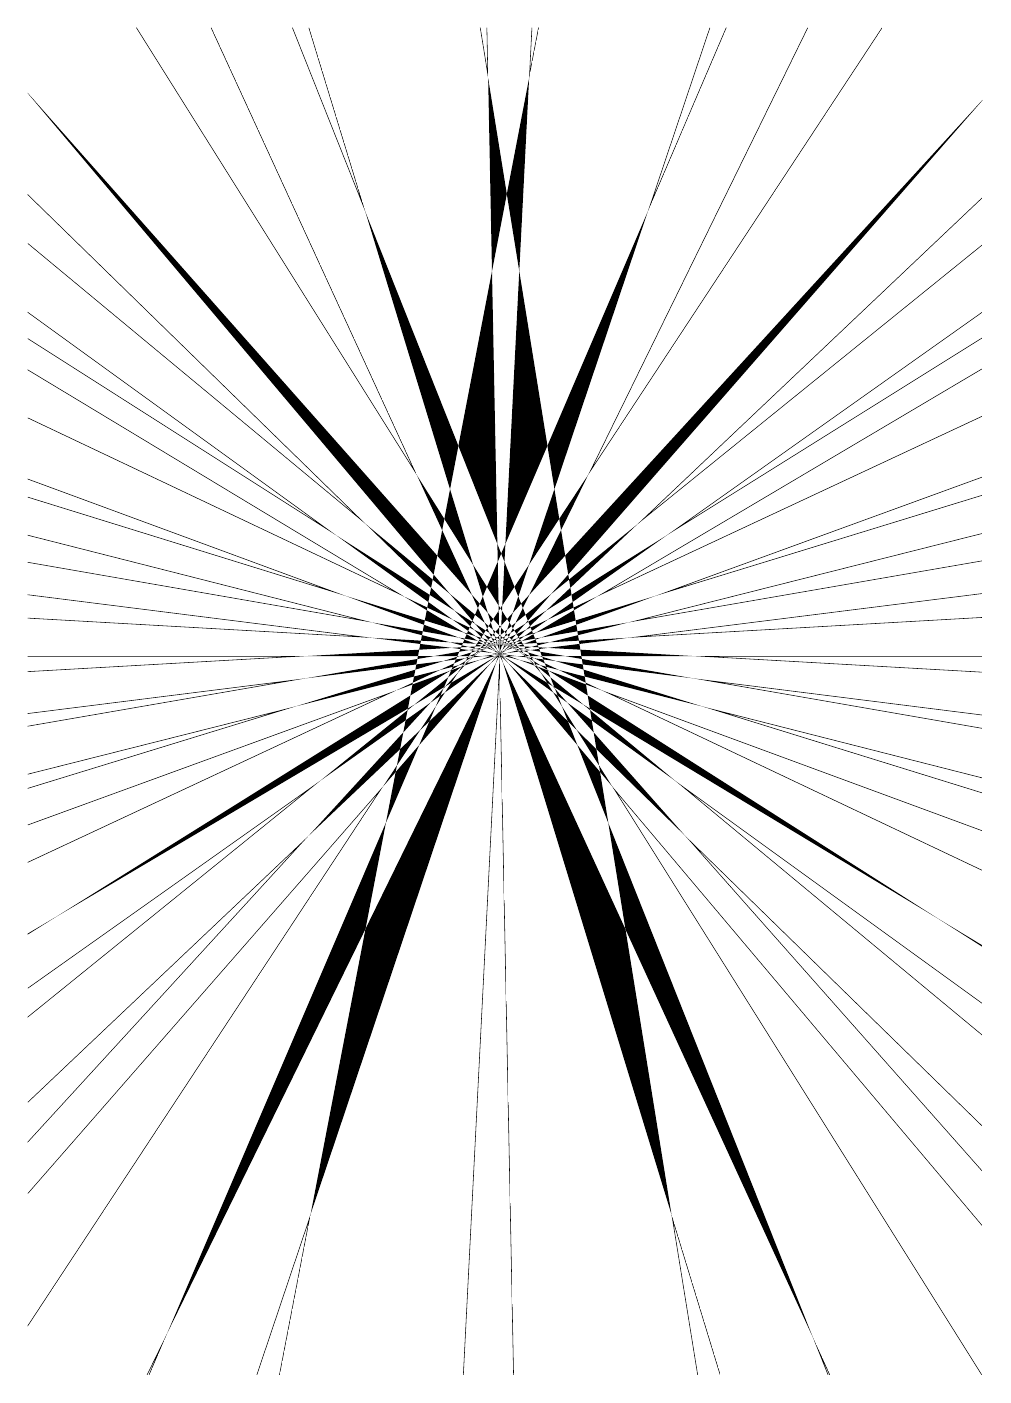
\begin{tikzpicture}[x=\linewidth,y=\linewidth]
\useasboundingbox (0,0) rectangle (1,1.41106);
\clip (0,0) rectangle (1,1.41106);
% External black cell outlines (inset)
\begin{scope}\clip (0.45604,0.00000) -- (0.50920,0.00000) -- (0.49431,0.75174) -- cycle; \draw[line width=0.4pt] (0.50920,0.00000) -- (0.49431,0.75174) (0.49431,0.75174) -- (0.45604,0.00000);\end{scope}
\begin{scope}\clip (0.72561,0.00000) -- (0.67432,0.16797) -- (0.70143,0.00000) -- cycle; \draw[line width=0.4pt] (0.72561,0.00000) -- (0.67432,0.16797) (0.67432,0.16797) -- (0.70143,0.00000);\end{scope}
\begin{scope}\clip (0.84043,0.00000) -- (0.82229,0.03950) -- (0.83800,0.00000) -- cycle; \draw[line width=0.4pt] (0.84043,0.00000) -- (0.82229,0.03950) (0.82229,0.03950) -- (0.83800,0.00000);\end{scope}
\begin{scope}\clip (1.00000,0.00000) -- (1.00000,0.15648) -- (0.61207,0.61656) -- (0.99897,0.00000) -- cycle; \draw[line width=0.4pt] (1.00000,0.15648) -- (0.61207,0.61656) (0.61207,0.61656) -- (0.99897,0.00000);\end{scope}
\begin{scope}\clip (1.00000,0.26080) -- (0.68836,0.56492) -- (1.00000,0.21277) -- cycle; \draw[line width=0.4pt] (1.00000,0.26080) -- (0.68836,0.56492) (0.68836,0.56492) -- (1.00000,0.21277);\end{scope}
\begin{scope}\clip (1.00000,0.38926) -- (0.67800,0.62241) -- (1.00000,0.35532) -- cycle; \draw[line width=0.4pt] (1.00000,0.38926) -- (0.67800,0.62241) (0.67800,0.62241) -- (1.00000,0.35532);\end{scope}
\begin{scope}\clip (1.00000,0.44985) -- (0.95355,0.47786) -- (1.00000,0.44829) -- cycle; \draw[line width=0.4pt] (1.00000,0.44985) -- (0.95355,0.47786) (0.95355,0.47786) -- (1.00000,0.44829);\end{scope}
\begin{scope}\clip (1.00000,0.57012) -- (0.60115,0.71709) -- (1.00000,0.52800) -- cycle; \draw[line width=0.4pt] (1.00000,0.57012) -- (0.60115,0.71709) (0.60115,0.71709) -- (1.00000,0.52800);\end{scope}
\begin{scope}\clip (1.00000,0.62551) -- (0.70646,0.70015) -- (1.00000,0.60919) -- cycle; \draw[line width=0.4pt] (1.00000,0.62551) -- (0.70646,0.70015) (0.70646,0.70015) -- (1.00000,0.60919);\end{scope}
\begin{scope}\clip (1.00000,0.69137) -- (0.69651,0.72962) -- (1.00000,0.67682) -- cycle; \draw[line width=0.4pt] (1.00000,0.69137) -- (0.69651,0.72962) (0.69651,0.72962) -- (1.00000,0.67682);\end{scope}
\begin{scope}\clip (1.00000,0.75276) -- (0.69897,0.75276) -- (1.00000,0.73571) -- cycle; \draw[line width=0.4pt] (1.00000,0.75276) -- (0.69897,0.75276) (0.69897,0.75276) -- (1.00000,0.73571);\end{scope}
\begin{scope}\clip (1.00000,0.81866) -- (0.62842,0.77195) -- (1.00000,0.79305) -- cycle; \draw[line width=0.4pt] (1.00000,0.81866) -- (0.62842,0.77195) (0.62842,0.77195) -- (1.00000,0.79305);\end{scope}
\begin{scope}\clip (1.00000,0.88162) -- (0.62927,0.78811) -- (1.00000,0.85234) -- cycle; \draw[line width=0.4pt] (1.00000,0.88162) -- (0.62927,0.78811) (0.62927,0.78811) -- (1.00000,0.85234);\end{scope}
\begin{scope}\clip (1.00000,0.94072) -- (0.65720,0.81578) -- (1.00000,0.92105) -- cycle; \draw[line width=0.4pt] (1.00000,0.94072) -- (0.65720,0.81578) (0.65720,0.81578) -- (1.00000,0.92105);\end{scope}
\begin{scope}\clip (1.00000,1.05423) -- (0.59612,0.81510) -- (1.00000,1.00388) -- cycle; \draw[line width=0.4pt] (1.00000,1.05423) -- (0.59612,0.81510) (0.59612,0.81510) -- (1.00000,1.00388);\end{scope}
\begin{scope}\clip (1.00000,1.11353) -- (0.66945,0.87939) -- (1.00000,1.08591) -- cycle; \draw[line width=0.4pt] (1.00000,1.11353) -- (0.66945,0.87939) (0.66945,0.87939) -- (1.00000,1.08591);\end{scope}
\begin{scope}\clip (1.00000,1.23346) -- (0.63839,0.89075) -- (1.00000,1.18329) -- cycle; \draw[line width=0.4pt] (1.00000,1.23346) -- (0.63839,0.89075) (0.63839,0.89075) -- (1.00000,1.18329);\end{scope}
\begin{scope}\clip (0.81675,1.41106) -- (0.58703,0.94264) -- (0.89533,1.41106) -- cycle; \draw[line width=0.4pt] (0.81675,1.41106) -- (0.58703,0.94264) (0.58703,0.94264) -- (0.89533,1.41106);\end{scope}
\begin{scope}\clip (0.71427,1.41106) -- (0.64954,1.21858) -- (0.73200,1.41106) -- cycle; \draw[line width=0.4pt] (0.71427,1.41106) -- (0.64954,1.21858) (0.64954,1.21858) -- (0.73200,1.41106);\end{scope}
\begin{scope}\clip (0.52787,1.41106) -- (0.52518,1.35808) -- (0.53537,1.41106) -- cycle; \draw[line width=0.4pt] (0.52787,1.41106) -- (0.52518,1.35808) (0.52518,1.35808) -- (0.53537,1.41106);\end{scope}
\begin{scope}\clip (0.23971,0.00000) -- (0.26400,0.00000) -- (0.29644,0.16869) -- cycle; \draw[line width=0.4pt] (0.26400,0.00000) -- (0.29644,0.16869) (0.29644,0.16869) -- (0.23971,0.00000);\end{scope}
\begin{scope}\clip (0.12476,0.00000) -- (0.12746,-0.00000) -- (0.14613,0.04359) -- cycle; \draw[line width=0.4pt] (0.12746,-0.00000) -- (0.14613,0.04359) (0.14613,0.04359) -- (0.12476,0.00000);\end{scope}
\begin{scope}\clip (0.00000,0.19023) -- (0.00000,0.05071) -- (0.37235,0.61646) -- cycle; \draw[line width=0.4pt] (0.00000,0.05071) -- (0.37235,0.61646) (0.37235,0.61646) -- (0.00000,0.19023);\end{scope}
\begin{scope}\clip (0.00000,0.24331) -- (0.29417,0.56454) -- (0.00000,0.28575) -- cycle; \draw[line width=0.4pt] (0.00000,0.24331) -- (0.29417,0.56454) (0.29417,0.56454) -- (0.00000,0.28575);\end{scope}
\begin{scope}\clip (0.00000,0.37432) -- (0.30690,0.62260) -- (0.00000,0.40521) -- cycle; \draw[line width=0.4pt] (0.00000,0.37432) -- (0.30690,0.62260) (0.30690,0.62260) -- (0.00000,0.40521);\end{scope}
\begin{scope}\clip (0.00000,0.46115) -- (0.03085,0.48042) -- (0.00000,0.46215) -- cycle; \draw[line width=0.4pt] (0.00000,0.46115) -- (0.03085,0.48042) (0.03085,0.48042) -- (0.00000,0.46215);\end{scope}
\begin{scope}\clip (0.00000,0.53646) -- (0.38643,0.71709) -- (0.00000,0.57624) -- cycle; \draw[line width=0.4pt] (0.00000,0.53646) -- (0.38643,0.71709) (0.38643,0.71709) -- (0.00000,0.57624);\end{scope}
\begin{scope}\clip (0.00000,0.61395) -- (0.28142,0.70038) -- (0.00000,0.62940) -- cycle; \draw[line width=0.4pt] (0.00000,0.61395) -- (0.28142,0.70038) (0.28142,0.70038) -- (0.00000,0.62940);\end{scope}
\begin{scope}\clip (0.00000,0.67910) -- (0.29147,0.72959) -- (0.00000,0.69295) -- cycle; \draw[line width=0.4pt] (0.00000,0.67910) -- (0.29147,0.72959) (0.29147,0.72959) -- (0.00000,0.69295);\end{scope}
\begin{scope}\clip (-0.00000,0.73626) -- (0.29058,0.75276) -- (0.00000,0.75276) -- cycle; \draw[line width=0.4pt] (-0.00000,0.73626) -- (0.29058,0.75276) (0.29058,0.75276) -- (0.00000,0.75276);\end{scope}
\begin{scope}\clip (-0.00000,0.79235) -- (0.36096,0.77191) -- (0.00000,0.81740) -- cycle; \draw[line width=0.4pt] (-0.00000,0.79235) -- (0.36096,0.77191) (0.36096,0.77191) -- (0.00000,0.81740);\end{scope}
\begin{scope}\clip (0.00000,0.85081) -- (0.36088,0.78802) -- (0.00000,0.87978) -- cycle; \draw[line width=0.4pt] (0.00000,0.85081) -- (0.36088,0.78802) (0.36088,0.78802) -- (0.00000,0.87978);\end{scope}
\begin{scope}\clip (0.00000,0.91906) -- (0.33344,0.81574) -- (0.00000,0.93861) -- cycle; \draw[line width=0.4pt] (0.00000,0.91906) -- (0.33344,0.81574) (0.33344,0.81574) -- (0.00000,0.93861);\end{scope}
\begin{scope}\clip (0.00000,1.00209) -- (0.39467,0.81498) -- (0.00000,1.05305) -- cycle; \draw[line width=0.4pt] (0.00000,1.00209) -- (0.39467,0.81498) (0.39467,0.81498) -- (0.00000,1.05305);\end{scope}
\begin{scope}\clip (-0.00000,1.08513) -- (0.32339,0.87918) -- (0.00000,1.11335) -- cycle; \draw[line width=0.4pt] (-0.00000,1.08513) -- (0.32339,0.87918) (0.32339,0.87918) -- (0.00000,1.11335);\end{scope}
\begin{scope}\clip (0.00000,1.18480) -- (0.35435,0.89088) -- (0.00000,1.23667) -- cycle; \draw[line width=0.4pt] (0.00000,1.18480) -- (0.35435,0.89088) (0.35435,0.89088) -- (0.00000,1.23667);\end{scope}
\begin{scope}\clip (0.11351,1.41106) -- (0.40778,0.94211) -- (0.19242,1.41106) -- cycle; \draw[line width=0.4pt] (0.11351,1.41106) -- (0.40778,0.94211) (0.40778,0.94211) -- (0.19242,1.41106);\end{scope}
\begin{scope}\clip (0.27696,1.41106) -- (0.35377,1.21789) -- (0.29479,1.41106) -- cycle; \draw[line width=0.4pt] (0.27696,1.41106) -- (0.35377,1.21789) (0.35377,1.21789) -- (0.29479,1.41106);\end{scope}
\begin{scope}\clip (0.47373,1.41106) -- (0.48231,1.35792) -- (0.48125,1.41106) -- cycle; \draw[line width=0.4pt] (0.47373,1.41106) -- (0.48231,1.35792) (0.48231,1.35792) -- (0.48125,1.41106);\end{scope}
% Filled cells
\fill (0.49784,0.74599) -- (0.67432,0.16797) -- (0.62613,0.46666) -- cycle;
\fill (0.49474,0.75276) -- (0.49784,0.74599) -- (0.49578,0.75276) -- cycle;
\fill (0.60814,0.57812) -- (0.62613,0.46666) -- (0.82229,0.03950) -- cycle;
\fill (0.57571,0.65968) -- (0.60814,0.57812) -- (0.59954,0.63142) -- cycle;
\fill (0.50351,0.74531) -- (0.57571,0.65968) -- (0.56586,0.68447) -- cycle;
\fill (0.59843,0.63830) -- (0.59954,0.63142) -- (0.61207,0.61656) -- cycle;
\fill (0.57514,0.67541) -- (0.59843,0.63830) -- (0.59567,0.65537) -- cycle;
\fill (0.49587,0.75276) -- (0.50351,0.74531) -- (0.49722,0.75276) -- cycle;
\fill (0.55963,0.70013) -- (0.56586,0.68447) -- (0.57514,0.67541) -- cycle;
\fill (0.55043,0.71478) -- (0.55963,0.70013) -- (0.55516,0.71136) -- cycle;
\fill (0.59286,0.67284) -- (0.59567,0.65537) -- (0.68836,0.56492) -- cycle;
\fill (0.56519,0.70410) -- (0.59286,0.67284) -- (0.59080,0.68555) -- cycle;
\fill (0.49879,0.75218) -- (0.55043,0.71478) -- (0.54413,0.72483) -- cycle;
\fill (0.55223,0.71875) -- (0.55516,0.71136) -- (0.56519,0.70410) -- cycle;
\fill (0.54995,0.72132) -- (0.55223,0.71875) -- (0.55160,0.72032) -- cycle;
\fill (0.58909,0.69616) -- (0.59080,0.68555) -- (0.67800,0.62241) -- cycle;
\fill (0.58226,0.70183) -- (0.58909,0.69616) -- (0.58882,0.69787) -- cycle;
\fill (0.49782,0.75276) -- (0.49879,0.75218) -- (0.49798,0.75276) -- cycle;
\fill (0.53751,0.73538) -- (0.54413,0.72483) -- (0.54995,0.72132) -- cycle;
\fill (0.53073,0.74304) -- (0.53751,0.73538) -- (0.53329,0.74210) -- cycle;
\fill (0.54748,0.73067) -- (0.55160,0.72032) -- (0.58226,0.70183) -- cycle;
\fill (0.53405,0.74182) -- (0.54748,0.73067) -- (0.54460,0.73793) -- cycle;
\fill (0.58661,0.71155) -- (0.58882,0.69787) -- (0.95355,0.47786) -- cycle;
\fill (0.54600,0.73742) -- (0.58661,0.71155) -- (0.58474,0.72314) -- cycle;
\fill (0.51507,0.74881) -- (0.53073,0.74304) -- (0.52868,0.74535) -- cycle;
\fill (0.53284,0.74282) -- (0.53329,0.74210) -- (0.53405,0.74182) -- cycle;
\fill (0.53028,0.74495) -- (0.53284,0.74282) -- (0.53174,0.74457) -- cycle;
\fill (0.54440,0.73843) -- (0.54460,0.73793) -- (0.54600,0.73742) -- cycle;
\fill (0.53676,0.74330) -- (0.54440,0.73843) -- (0.54311,0.74168) -- cycle;
\fill (0.58444,0.72502) -- (0.58474,0.72314) -- (0.60115,0.71709) -- cycle;
\fill (0.55642,0.73830) -- (0.58444,0.72502) -- (0.58340,0.73144) -- cycle;
\fill (0.49953,0.75276) -- (0.51507,0.74881) -- (0.50434,0.75276) -- cycle;
\fill (0.52563,0.74880) -- (0.52868,0.74535) -- (0.53028,0.74495) -- cycle;
\fill (0.52228,0.75158) -- (0.52563,0.74880) -- (0.52328,0.75145) -- cycle;
\fill (0.52973,0.74778) -- (0.53174,0.74457) -- (0.53676,0.74330) -- cycle;
\fill (0.52412,0.75135) -- (0.52973,0.74778) -- (0.52778,0.75089) -- cycle;
\fill (0.54167,0.74529) -- (0.54311,0.74168) -- (0.55642,0.73830) -- cycle;
\fill (0.53063,0.75053) -- (0.54167,0.74529) -- (0.54006,0.74934) -- cycle;
\fill (0.58224,0.73864) -- (0.58340,0.73144) -- (0.70646,0.70015) -- cycle;
\fill (0.55297,0.74771) -- (0.58224,0.73864) -- (0.58135,0.74413) -- cycle;
\fill (0.51288,0.75276) -- (0.52228,0.75158) -- (0.52085,0.75276) -- cycle;
\fill (0.52241,0.75243) -- (0.52328,0.75145) -- (0.52412,0.75135) -- cycle;
\fill (0.52190,0.75276) -- (0.52241,0.75243) -- (0.52212,0.75276) -- cycle;
\fill (0.52689,0.75230) -- (0.52778,0.75089) -- (0.53063,0.75053) -- cycle;
\fill (0.52591,0.75276) -- (0.52689,0.75230) -- (0.52660,0.75276) -- cycle;
\fill (0.53899,0.75204) -- (0.54006,0.74934) -- (0.55297,0.74771) -- cycle;
\fill (0.53666,0.75276) -- (0.53899,0.75204) -- (0.53870,0.75276) -- cycle;
\fill (0.58043,0.74982) -- (0.58135,0.74413) -- (0.69651,0.72962) -- cycle;
\fill (0.56350,0.75276) -- (0.58043,0.74982) -- (0.57996,0.75276) -- cycle;
\fill (0.49436,0.75276) -- (0.49474,0.75276) -- (0.49440,0.75350) -- cycle;
\fill (0.49574,0.75290) -- (0.49578,0.75276) -- (0.49587,0.75276) -- cycle;
\fill (0.49458,0.75402) -- (0.49574,0.75290) -- (0.49546,0.75380) -- cycle;
\fill (0.49661,0.75349) -- (0.49722,0.75276) -- (0.49782,0.75276) -- cycle;
\fill (0.49657,0.75352) -- (0.49661,0.75349) -- (0.49660,0.75351) -- cycle;
\fill (0.49714,0.75337) -- (0.49798,0.75276) -- (0.49953,0.75276) -- cycle;
\fill (0.49454,0.75403) -- (0.49458,0.75402) -- (0.49455,0.75405) -- cycle;
\fill (0.49532,0.75427) -- (0.49546,0.75380) -- (0.49657,0.75352) -- cycle;
\fill (0.49525,0.75431) -- (0.49532,0.75427) -- (0.49530,0.75432) -- cycle;
\fill (0.49604,0.75417) -- (0.49660,0.75351) -- (0.49714,0.75337) -- cycle;
\fill (0.49569,0.75442) -- (0.49604,0.75417) -- (0.49580,0.75445) -- cycle;
\fill (0.49991,0.75440) -- (0.50434,0.75276) -- (0.51288,0.75276) -- cycle;
\fill (0.49704,0.75476) -- (0.49991,0.75440) -- (0.49816,0.75504) -- cycle;
\fill (0.51739,0.75563) -- (0.52085,0.75276) -- (0.52190,0.75276) -- cycle;
\fill (0.51430,0.75760) -- (0.51739,0.75563) -- (0.51492,0.75768) -- cycle;
\fill (0.51939,0.75586) -- (0.52212,0.75276) -- (0.52591,0.75276) -- cycle;
\fill (0.51541,0.75774) -- (0.51939,0.75586) -- (0.51749,0.75800) -- cycle;
\fill (0.52417,0.75664) -- (0.52660,0.75276) -- (0.53666,0.75276) -- cycle;
\fill (0.51910,0.75821) -- (0.52417,0.75664) -- (0.52288,0.75868) -- cycle;
\fill (0.53686,0.75740) -- (0.53870,0.75276) -- (0.56350,0.75276) -- cycle;
\fill (0.52671,0.75916) -- (0.53686,0.75740) -- (0.53571,0.76030) -- cycle;
\fill (0.57886,0.75957) -- (0.57996,0.75276) -- (0.69897,0.75276) -- cycle;
\fill (0.54512,0.76148) -- (0.57886,0.75957) -- (0.57789,0.76560) -- cycle;
\fill (0.50236,0.75610) -- (0.51430,0.75760) -- (0.51260,0.75869) -- cycle;
\fill (0.51410,0.75836) -- (0.51492,0.75768) -- (0.51541,0.75774) -- cycle;
\fill (0.51313,0.75882) -- (0.51410,0.75836) -- (0.51345,0.75890) -- cycle;
\fill (0.51663,0.75897) -- (0.51749,0.75800) -- (0.51910,0.75821) -- cycle;
\fill (0.51533,0.75937) -- (0.51663,0.75897) -- (0.51610,0.75957) -- cycle;
\fill (0.52208,0.75997) -- (0.52288,0.75868) -- (0.52671,0.75916) -- cycle;
\fill (0.51949,0.76042) -- (0.52208,0.75997) -- (0.52148,0.76092) -- cycle;
\fill (0.53501,0.76205) -- (0.53571,0.76030) -- (0.54512,0.76148) -- cycle;
\fill (0.52761,0.76247) -- (0.53501,0.76205) -- (0.53418,0.76413) -- cycle;
\fill (0.57733,0.76905) -- (0.57789,0.76560) -- (0.62842,0.77195) -- cycle;
\fill (0.54682,0.76732) -- (0.57733,0.76905) -- (0.57641,0.77478) -- cycle;
\fill (0.49459,0.75414) -- (0.49525,0.75431) -- (0.49481,0.75458) -- cycle;
\fill (0.49515,0.75481) -- (0.49530,0.75432) -- (0.49569,0.75442) -- cycle;
\fill (0.49503,0.75490) -- (0.49515,0.75481) -- (0.49510,0.75497) -- cycle;
\fill (0.49536,0.75497) -- (0.49580,0.75445) -- (0.49704,0.75476) -- cycle;
\fill (0.49514,0.75500) -- (0.49536,0.75497) -- (0.49525,0.75510) -- cycle;
\fill (0.49708,0.75544) -- (0.49816,0.75504) -- (0.50236,0.75610) -- cycle;
\fill (0.49538,0.75523) -- (0.49708,0.75544) -- (0.49602,0.75583) -- cycle;
\fill (0.51021,0.76021) -- (0.51260,0.75869) -- (0.51313,0.75882) -- cycle;
\fill (0.50783,0.76134) -- (0.51021,0.76021) -- (0.50822,0.76148) -- cycle;
\fill (0.51142,0.76059) -- (0.51345,0.75890) -- (0.51533,0.75937) -- cycle;
\fill (0.50837,0.76153) -- (0.51142,0.76059) -- (0.50970,0.76202) -- cycle;
\fill (0.51459,0.76127) -- (0.51610,0.75957) -- (0.51949,0.76042) -- cycle;
\fill (0.50990,0.76209) -- (0.51459,0.76127) -- (0.51290,0.76318) -- cycle;
\fill (0.52025,0.76289) -- (0.52148,0.76092) -- (0.52761,0.76247) -- cycle;
\fill (0.51319,0.76329) -- (0.52025,0.76289) -- (0.51873,0.76531) -- cycle;
\fill (0.53322,0.76654) -- (0.53418,0.76413) -- (0.54682,0.76732) -- cycle;
\fill (0.52007,0.76580) -- (0.53322,0.76654) -- (0.53182,0.77008) -- cycle;
\fill (0.57575,0.77884) -- (0.57641,0.77478) -- (0.62927,0.78811) -- cycle;
\fill (0.53784,0.77227) -- (0.57575,0.77884) -- (0.57465,0.78569) -- cycle;
\fill (0.50128,0.75895) -- (0.50783,0.76134) -- (0.50643,0.76200) -- cycle;
\fill (0.50790,0.76168) -- (0.50822,0.76148) -- (0.50837,0.76153) -- cycle;
\fill (0.50658,0.76209) -- (0.50790,0.76168) -- (0.50693,0.76229) -- cycle;
\fill (0.50953,0.76215) -- (0.50970,0.76202) -- (0.50990,0.76209) -- cycle;
\fill (0.50734,0.76254) -- (0.50953,0.76215) -- (0.50835,0.76313) -- cycle;
\fill (0.51279,0.76331) -- (0.51290,0.76318) -- (0.51319,0.76329) -- cycle;
\fill (0.50901,0.76352) -- (0.51279,0.76331) -- (0.51137,0.76492) -- cycle;
\fill (0.51848,0.76571) -- (0.51873,0.76531) -- (0.52007,0.76580) -- cycle;
\fill (0.51208,0.76534) -- (0.51848,0.76571) -- (0.51691,0.76820) -- cycle;
\fill (0.53139,0.77116) -- (0.53182,0.77008) -- (0.53784,0.77227) -- cycle;
\fill (0.51797,0.76883) -- (0.53139,0.77116) -- (0.52958,0.77570) -- cycle;
\fill (0.57392,0.79020) -- (0.57465,0.78569) -- (0.65720,0.81578) -- cycle;
\fill (0.53267,0.77754) -- (0.57392,0.79020) -- (0.57219,0.80093) -- cycle;
\fill (0.49602,0.75584) -- (0.50128,0.75895) -- (0.49807,0.75778) -- cycle;
\fill (0.50561,0.76239) -- (0.50643,0.76200) -- (0.50658,0.76209) -- cycle;
\fill (0.50467,0.76268) -- (0.50561,0.76239) -- (0.50480,0.76277) -- cycle;
\fill (0.50626,0.76272) -- (0.50693,0.76229) -- (0.50734,0.76254) -- cycle;
\fill (0.50503,0.76294) -- (0.50626,0.76272) -- (0.50546,0.76324) -- cycle;
\fill (0.50780,0.76359) -- (0.50835,0.76313) -- (0.50901,0.76352) -- cycle;
\fill (0.50610,0.76369) -- (0.50780,0.76359) -- (0.50695,0.76429) -- cycle;
\fill (0.51104,0.76528) -- (0.51137,0.76492) -- (0.51208,0.76534) -- cycle;
\fill (0.50811,0.76512) -- (0.51104,0.76528) -- (0.51000,0.76646) -- cycle;
\fill (0.51666,0.76860) -- (0.51691,0.76820) -- (0.51797,0.76883) -- cycle;
\fill (0.51186,0.76777) -- (0.51666,0.76860) -- (0.51554,0.77038) -- cycle;
\fill (0.52927,0.77649) -- (0.52958,0.77570) -- (0.53267,0.77754) -- cycle;
\fill (0.52026,0.77372) -- (0.52927,0.77649) -- (0.52815,0.77931) -- cycle;
\fill (0.57174,0.80370) -- (0.57219,0.80093) -- (0.59612,0.81510) -- cycle;
\fill (0.54484,0.79113) -- (0.57174,0.80370) -- (0.57080,0.80952) -- cycle;
\fill (0.49902,0.75868) -- (0.50467,0.76268) -- (0.50359,0.76301) -- cycle;
\fill (0.50412,0.76310) -- (0.50480,0.76277) -- (0.50503,0.76294) -- cycle;
\fill (0.50375,0.76316) -- (0.50412,0.76310) -- (0.50383,0.76323) -- cycle;
\fill (0.50461,0.76377) -- (0.50546,0.76324) -- (0.50610,0.76369) -- cycle;
\fill (0.50441,0.76378) -- (0.50461,0.76377) -- (0.50448,0.76385) -- cycle;
\fill (0.50610,0.76500) -- (0.50695,0.76429) -- (0.50811,0.76512) -- cycle;
\fill (0.50567,0.76498) -- (0.50610,0.76500) -- (0.50588,0.76518) -- cycle;
\fill (0.50924,0.76732) -- (0.51000,0.76646) -- (0.51186,0.76777) -- cycle;
\fill (0.50789,0.76708) -- (0.50924,0.76732) -- (0.50874,0.76789) -- cycle;
\fill (0.51455,0.77197) -- (0.51554,0.77038) -- (0.52026,0.77372) -- cycle;
\fill (0.51233,0.77129) -- (0.51455,0.77197) -- (0.51399,0.77286) -- cycle;
\fill (0.52680,0.78270) -- (0.52815,0.77931) -- (0.54484,0.79113) -- cycle;
\fill (0.52200,0.78046) -- (0.52680,0.78270) -- (0.52613,0.78437) -- cycle;
\fill (0.56959,0.81701) -- (0.57080,0.80952) -- (0.66945,0.87939) -- cycle;
\fill (0.54311,0.80047) -- (0.56959,0.81701) -- (0.56839,0.82442) -- cycle;
\fill (0.49490,0.75477) -- (0.49503,0.75490) -- (0.49498,0.75494) -- cycle;
\fill (0.49509,0.75501) -- (0.49510,0.75497) -- (0.49514,0.75500) -- cycle;
\fill (0.49502,0.75501) -- (0.49509,0.75501) -- (0.49506,0.75510) -- cycle;
\fill (0.49517,0.75520) -- (0.49525,0.75510) -- (0.49538,0.75523) -- cycle;
\fill (0.49511,0.75519) -- (0.49517,0.75520) -- (0.49513,0.75525) -- cycle;
\fill (0.49602,0.75583) -- (0.49602,0.75583) -- (0.49602,0.75584) -- cycle;
\fill (0.49518,0.75534) -- (0.49602,0.75583) -- (0.49551,0.75602) -- cycle;
\fill (0.49741,0.75754) -- (0.49807,0.75778) -- (0.49902,0.75868) -- cycle;
\fill (0.49564,0.75628) -- (0.49741,0.75754) -- (0.49601,0.75703) -- cycle;
\fill (0.50231,0.76341) -- (0.50359,0.76301) -- (0.50375,0.76316) -- cycle;
\fill (0.50094,0.76365) -- (0.50231,0.76341) -- (0.50107,0.76380) -- cycle;
\fill (0.50243,0.76390) -- (0.50383,0.76323) -- (0.50441,0.76378) -- cycle;
\fill (0.50121,0.76397) -- (0.50243,0.76390) -- (0.50153,0.76432) -- cycle;
\fill (0.50296,0.76483) -- (0.50448,0.76385) -- (0.50567,0.76498) -- cycle;
\fill (0.50191,0.76477) -- (0.50296,0.76483) -- (0.50232,0.76523) -- cycle;
\fill (0.50433,0.76647) -- (0.50588,0.76518) -- (0.50789,0.76708) -- cycle;
\fill (0.50323,0.76628) -- (0.50433,0.76647) -- (0.50379,0.76692) -- cycle;
\fill (0.50714,0.76969) -- (0.50874,0.76789) -- (0.51233,0.77129) -- cycle;
\fill (0.50588,0.76931) -- (0.50714,0.76969) -- (0.50668,0.77022) -- cycle;
\fill (0.51212,0.77584) -- (0.51399,0.77286) -- (0.52200,0.78046) -- cycle;
\fill (0.51122,0.77542) -- (0.51212,0.77584) -- (0.51190,0.77619) -- cycle;
\fill (0.52439,0.78877) -- (0.52613,0.78437) -- (0.54311,0.80047) -- cycle;
\fill (0.52107,0.78669) -- (0.52439,0.78877) -- (0.52392,0.78995) -- cycle;
\fill (0.56701,0.83301) -- (0.56839,0.82442) -- (0.63839,0.89075) -- cycle;
\fill (0.54834,0.81791) -- (0.56701,0.83301) -- (0.56616,0.83830) -- cycle;
\fill (0.49710,0.75926) -- (0.50094,0.76365) -- (0.49939,0.76392) -- cycle;
\fill (0.50036,0.76401) -- (0.50107,0.76380) -- (0.50121,0.76397) -- cycle;
\fill (0.49946,0.76406) -- (0.50036,0.76401) -- (0.49956,0.76426) -- cycle;
\fill (0.50073,0.76470) -- (0.50153,0.76432) -- (0.50191,0.76477) -- cycle;
\fill (0.49974,0.76464) -- (0.50073,0.76470) -- (0.49995,0.76507) -- cycle;
\fill (0.50122,0.76593) -- (0.50232,0.76523) -- (0.50323,0.76628) -- cycle;
\fill (0.50029,0.76577) -- (0.50122,0.76593) -- (0.50058,0.76634) -- cycle;
\fill (0.50225,0.76819) -- (0.50379,0.76692) -- (0.50588,0.76931) -- cycle;
\fill (0.50135,0.76792) -- (0.50225,0.76819) -- (0.50170,0.76865) -- cycle;
\fill (0.50475,0.77239) -- (0.50668,0.77022) -- (0.51122,0.77542) -- cycle;
\fill (0.50318,0.77166) -- (0.50475,0.77239) -- (0.50397,0.77327) -- cycle;
\fill (0.50975,0.77962) -- (0.51190,0.77619) -- (0.52107,0.78669) -- cycle;
\fill (0.50591,0.77722) -- (0.50975,0.77962) -- (0.50825,0.78200) -- cycle;
\fill (0.52145,0.79616) -- (0.52392,0.78995) -- (0.54834,0.81791) -- cycle;
\fill (0.51108,0.78777) -- (0.52145,0.79616) -- (0.51865,0.80320) -- cycle;
\fill (1.00000,1.33530) -- (0.56297,0.85806) -- (0.56616,0.83830) -- (1.00000,1.33492) -- cycle;
\fill (0.52548,0.81713) -- (0.56297,0.85806) -- (0.55866,0.88478) -- cycle;
\fill (0.49441,0.75378) -- (0.49454,0.75403) -- (0.49443,0.75406) -- cycle;
\fill (0.49449,0.75412) -- (0.49455,0.75405) -- (0.49459,0.75414) -- cycle;
\fill (0.49443,0.75410) -- (0.49449,0.75412) -- (0.49443,0.75417) -- cycle;
\fill (0.49474,0.75462) -- (0.49481,0.75458) -- (0.49490,0.75477) -- cycle;
\fill (0.49444,0.75434) -- (0.49474,0.75462) -- (0.49447,0.75479) -- cycle;
\fill (0.49484,0.75504) -- (0.49498,0.75494) -- (0.49502,0.75501) -- cycle;
\fill (0.49470,0.75505) -- (0.49484,0.75504) -- (0.49477,0.75509) -- cycle;
\fill (0.49504,0.75518) -- (0.49506,0.75510) -- (0.49511,0.75519) -- cycle;
\fill (0.49489,0.75516) -- (0.49504,0.75518) -- (0.49502,0.75524) -- cycle;
\fill (0.49510,0.75529) -- (0.49513,0.75525) -- (0.49518,0.75534) -- cycle;
\fill (0.49447,0.75492) -- (0.49470,0.75505) -- (0.49448,0.75508) -- cycle;
\fill (0.49470,0.75514) -- (0.49477,0.75509) -- (0.49489,0.75516) -- cycle;
\fill (0.49448,0.75511) -- (0.49470,0.75514) -- (0.49449,0.75529) -- cycle;
\fill (0.49496,0.75546) -- (0.49502,0.75524) -- (0.49510,0.75529) -- cycle;
\fill (0.49477,0.75567) -- (0.49496,0.75546) -- (0.49487,0.75574) -- cycle;
\fill (0.49535,0.75608) -- (0.49551,0.75602) -- (0.49564,0.75628) -- cycle;
\fill (0.49450,0.75548) -- (0.49477,0.75567) -- (0.49453,0.75597) -- cycle;
\fill (0.49469,0.75632) -- (0.49487,0.75574) -- (0.49535,0.75608) -- cycle;
\fill (0.49457,0.75636) -- (0.49469,0.75632) -- (0.49465,0.75645) -- cycle;
\fill (0.49475,0.75657) -- (0.49601,0.75703) -- (0.49710,0.75926) -- cycle;
\fill (0.49454,0.75633) -- (0.49457,0.75636) -- (0.49455,0.75637) -- cycle;
\fill (0.49463,0.75652) -- (0.49465,0.75645) -- (0.49475,0.75657) -- cycle;
\fill (0.49455,0.75650) -- (0.49463,0.75652) -- (0.49456,0.75674) -- cycle;
\fill (0.49811,0.76414) -- (0.49939,0.76392) -- (0.49946,0.76406) -- cycle;
\fill (0.49673,0.76422) -- (0.49811,0.76414) -- (0.49678,0.76437) -- cycle;
\fill (0.49855,0.76458) -- (0.49956,0.76426) -- (0.49974,0.76464) -- cycle;
\fill (0.49681,0.76448) -- (0.49855,0.76458) -- (0.49701,0.76505) -- cycle;
\fill (0.49896,0.76554) -- (0.49995,0.76507) -- (0.50029,0.76577) -- cycle;
\fill (0.49706,0.76521) -- (0.49896,0.76554) -- (0.49742,0.76627) -- cycle;
\fill (0.49916,0.76724) -- (0.50058,0.76634) -- (0.50135,0.76792) -- cycle;
\fill (0.49758,0.76676) -- (0.49916,0.76724) -- (0.49799,0.76799) -- cycle;
\fill (0.49991,0.77013) -- (0.50170,0.76865) -- (0.50318,0.77166) -- cycle;
\fill (0.49849,0.76947) -- (0.49991,0.77013) -- (0.49898,0.77091) -- cycle;
\fill (0.50241,0.77504) -- (0.50397,0.77327) -- (0.50591,0.77722) -- cycle;
\fill (0.49982,0.77342) -- (0.50241,0.77504) -- (0.50093,0.77671) -- cycle;
\fill (0.50680,0.78431) -- (0.50825,0.78200) -- (0.51108,0.78777) -- cycle;
\fill (0.50224,0.78062) -- (0.50680,0.78431) -- (0.50464,0.78775) -- cycle;
\fill (0.51686,0.80771) -- (0.51865,0.80320) -- (0.52548,0.81713) -- cycle;
\fill (0.50816,0.79821) -- (0.51686,0.80771) -- (0.51388,0.81520) -- cycle;
\fill (0.55674,0.89662) -- (0.55866,0.88478) -- (0.58703,0.94264) -- cycle;
\fill (0.52507,0.84850) -- (0.55674,0.89662) -- (0.55172,0.92774) -- cycle;
\fill (0.49463,0.75797) -- (0.49673,0.76422) -- (0.49495,0.76432) -- cycle;
\fill (0.49634,0.76445) -- (0.49678,0.76437) -- (0.49681,0.76448) -- cycle;
\fill (0.49495,0.76437) -- (0.49634,0.76445) -- (0.49497,0.76469) -- cycle;
\fill (0.49671,0.76515) -- (0.49701,0.76505) -- (0.49706,0.76521) -- cycle;
\fill (0.49498,0.76485) -- (0.49671,0.76515) -- (0.49502,0.76567) -- cycle;
\fill (0.49686,0.76654) -- (0.49742,0.76627) -- (0.49758,0.76676) -- cycle;
\fill (0.49503,0.76598) -- (0.49686,0.76654) -- (0.49511,0.76737) -- cycle;
\fill (0.49686,0.76871) -- (0.49799,0.76799) -- (0.49849,0.76947) -- cycle;
\fill (0.49513,0.76790) -- (0.49686,0.76871) -- (0.49523,0.76975) -- cycle;
\fill (0.49761,0.77204) -- (0.49898,0.77091) -- (0.49982,0.77342) -- cycle;
\fill (0.49527,0.77057) -- (0.49761,0.77204) -- (0.49544,0.77385) -- cycle;
\fill (0.49946,0.77837) -- (0.50093,0.77671) -- (0.50224,0.78062) -- cycle;
\fill (0.49550,0.77517) -- (0.49946,0.77837) -- (0.49587,0.78243) -- cycle;
\fill (0.50218,0.79168) -- (0.50464,0.78775) -- (0.50816,0.79821) -- cycle;
\fill (0.49600,0.78493) -- (0.50218,0.79168) -- (0.49678,0.80028) -- cycle;
\fill (0.50984,0.82535) -- (0.51388,0.81520) -- (0.52507,0.84850) -- cycle;
\fill (0.49707,0.80595) -- (0.50984,0.82535) -- (0.49939,0.85162) -- cycle;
\fill (0.54439,0.97316) -- (0.55172,0.92774) -- (0.64954,1.21858) -- cycle;
\fill (0.50035,0.87036) -- (0.54439,0.97316) -- (0.51489,1.15600) -- cycle;
\fill (0.49429,0.75276) -- (0.49431,0.75174) -- (0.49436,0.75276) -- cycle;
\fill (0.49392,0.75276) -- (0.49429,0.75276) -- (0.49428,0.75350) -- cycle;
\fill (0.49434,0.75363) -- (0.49440,0.75350) -- (0.49441,0.75378) -- cycle;
\fill (0.49060,0.74601) -- (0.49392,0.75276) -- (0.49288,0.75276) -- cycle;
\fill (0.49427,0.75378) -- (0.49428,0.75350) -- (0.49434,0.75363) -- cycle;
\fill (0.49415,0.75403) -- (0.49427,0.75378) -- (0.49426,0.75406) -- cycle;
\fill (0.49435,0.75408) -- (0.49443,0.75406) -- (0.49443,0.75410) -- cycle;
\fill (0.49411,0.75402) -- (0.49415,0.75403) -- (0.49414,0.75405) -- cycle;
\fill (0.49426,0.75410) -- (0.49426,0.75406) -- (0.49435,0.75408) -- cycle;
\fill (0.49421,0.75412) -- (0.49426,0.75410) -- (0.49426,0.75417) -- cycle;
\fill (0.49435,0.75425) -- (0.49443,0.75417) -- (0.49444,0.75434) -- cycle;
\fill (0.49292,0.75289) -- (0.49411,0.75402) -- (0.49322,0.75380) -- cycle;
\fill (0.49410,0.75414) -- (0.49414,0.75405) -- (0.49421,0.75412) -- cycle;
\fill (0.49345,0.75431) -- (0.49410,0.75414) -- (0.49390,0.75458) -- cycle;
\fill (0.49426,0.75434) -- (0.49426,0.75417) -- (0.49435,0.75425) -- cycle;
\fill (0.49397,0.75462) -- (0.49426,0.75434) -- (0.49425,0.75479) -- cycle;
\fill (0.49436,0.75485) -- (0.49447,0.75479) -- (0.49447,0.75492) -- cycle;
\fill (0.49338,0.75427) -- (0.49345,0.75431) -- (0.49340,0.75432) -- cycle;
\fill (0.49381,0.75477) -- (0.49390,0.75458) -- (0.49397,0.75462) -- cycle;
\fill (0.49369,0.75490) -- (0.49381,0.75477) -- (0.49374,0.75494) -- cycle;
\fill (0.49425,0.75492) -- (0.49425,0.75479) -- (0.49436,0.75485) -- cycle;
\fill (0.49402,0.75505) -- (0.49425,0.75492) -- (0.49424,0.75508) -- cycle;
\fill (0.49436,0.75510) -- (0.49448,0.75508) -- (0.49448,0.75511) -- cycle;
\fill (0.49388,0.75504) -- (0.49402,0.75505) -- (0.49396,0.75509) -- cycle;
\fill (0.49424,0.75511) -- (0.49424,0.75508) -- (0.49436,0.75510) -- cycle;
\fill (0.49403,0.75514) -- (0.49424,0.75511) -- (0.49424,0.75529) -- cycle;
\fill (0.49437,0.75538) -- (0.49449,0.75529) -- (0.49450,0.75548) -- cycle;
\fill (0.49356,0.75481) -- (0.49369,0.75490) -- (0.49362,0.75497) -- cycle;
\fill (0.49370,0.75501) -- (0.49374,0.75494) -- (0.49388,0.75504) -- cycle;
\fill (0.49363,0.75501) -- (0.49370,0.75501) -- (0.49366,0.75510) -- cycle;
\fill (0.49384,0.75516) -- (0.49396,0.75509) -- (0.49403,0.75514) -- cycle;
\fill (0.49369,0.75518) -- (0.49384,0.75516) -- (0.49371,0.75524) -- cycle;
\fill (0.49424,0.75548) -- (0.49424,0.75529) -- (0.49437,0.75538) -- cycle;
\fill (0.49397,0.75567) -- (0.49424,0.75548) -- (0.49423,0.75597) -- cycle;
\fill (0.49438,0.75614) -- (0.49453,0.75597) -- (0.49454,0.75633) -- cycle;
\fill (0.49378,0.75546) -- (0.49397,0.75567) -- (0.49387,0.75574) -- cycle;
\fill (0.49422,0.75633) -- (0.49423,0.75597) -- (0.49438,0.75614) -- cycle;
\fill (0.49419,0.75636) -- (0.49422,0.75633) -- (0.49422,0.75637) -- cycle;
\fill (0.49438,0.75643) -- (0.49455,0.75637) -- (0.49455,0.75650) -- cycle;
\fill (0.49407,0.75632) -- (0.49419,0.75636) -- (0.49412,0.75645) -- cycle;
\fill (0.49422,0.75650) -- (0.49422,0.75637) -- (0.49438,0.75643) -- cycle;
\fill (0.49414,0.75652) -- (0.49422,0.75650) -- (0.49421,0.75674) -- cycle;
\fill (0.49440,0.75729) -- (0.49456,0.75674) -- (0.49463,0.75797) -- cycle;
\fill (0.29644,0.16869) -- (0.49060,0.74601) -- (0.35383,0.46711) -- cycle;
\fill (0.49278,0.75276) -- (0.49288,0.75276) -- (0.49292,0.75289) -- cycle;
\fill (0.48492,0.74532) -- (0.49278,0.75276) -- (0.49143,0.75276) -- cycle;
\fill (0.49210,0.75352) -- (0.49322,0.75380) -- (0.49338,0.75427) -- cycle;
\fill (0.49207,0.75349) -- (0.49210,0.75352) -- (0.49208,0.75351) -- cycle;
\fill (0.49301,0.75442) -- (0.49340,0.75432) -- (0.49356,0.75481) -- cycle;
\fill (0.49266,0.75417) -- (0.49301,0.75442) -- (0.49290,0.75445) -- cycle;
\fill (0.49358,0.75500) -- (0.49362,0.75497) -- (0.49363,0.75501) -- cycle;
\fill (0.49336,0.75497) -- (0.49358,0.75500) -- (0.49347,0.75510) -- cycle;
\fill (0.49362,0.75519) -- (0.49366,0.75510) -- (0.49369,0.75518) -- cycle;
\fill (0.49356,0.75520) -- (0.49362,0.75519) -- (0.49360,0.75524) -- cycle;
\fill (0.49363,0.75529) -- (0.49371,0.75524) -- (0.49378,0.75546) -- cycle;
\fill (0.41007,0.65963) -- (0.48492,0.74532) -- (0.42070,0.68445) -- cycle;
\fill (0.49084,0.75276) -- (0.49143,0.75276) -- (0.49207,0.75349) -- cycle;
\fill (0.48985,0.75218) -- (0.49084,0.75276) -- (0.49067,0.75276) -- cycle;
\fill (0.49153,0.75337) -- (0.49208,0.75351) -- (0.49266,0.75417) -- cycle;
\fill (0.43708,0.71480) -- (0.48985,0.75218) -- (0.44369,0.72485) -- cycle;
\fill (0.48913,0.75276) -- (0.49067,0.75276) -- (0.49153,0.75337) -- cycle;
\fill (0.47350,0.74882) -- (0.48913,0.75276) -- (0.48431,0.75276) -- cycle;
\fill (0.49168,0.75476) -- (0.49290,0.75445) -- (0.49336,0.75497) -- cycle;
\fill (0.48880,0.75440) -- (0.49168,0.75476) -- (0.49056,0.75504) -- cycle;
\fill (0.49335,0.75523) -- (0.49347,0.75510) -- (0.49356,0.75520) -- cycle;
\fill (0.49165,0.75544) -- (0.49335,0.75523) -- (0.49273,0.75583) -- cycle;
\fill (0.49355,0.75534) -- (0.49360,0.75524) -- (0.49363,0.75529) -- cycle;
\fill (0.49273,0.75583) -- (0.49355,0.75534) -- (0.49324,0.75602) -- cycle;
\fill (0.49340,0.75608) -- (0.49387,0.75574) -- (0.49407,0.75632) -- cycle;
\fill (0.45763,0.74304) -- (0.47350,0.74882) -- (0.45976,0.74536) -- cycle;
\fill (0.47580,0.75276) -- (0.48431,0.75276) -- (0.48880,0.75440) -- cycle;
\fill (0.46634,0.75157) -- (0.47580,0.75276) -- (0.46781,0.75276) -- cycle;
\fill (0.48641,0.75610) -- (0.49056,0.75504) -- (0.49165,0.75544) -- cycle;
\fill (0.47451,0.75760) -- (0.48641,0.75610) -- (0.47624,0.75868) -- cycle;
\fill (0.49272,0.75584) -- (0.49273,0.75583) -- (0.49273,0.75583) -- cycle;
\fill (0.48757,0.75894) -- (0.49272,0.75584) -- (0.49073,0.75778) -- cycle;
\fill (0.49312,0.75628) -- (0.49324,0.75602) -- (0.49340,0.75608) -- cycle;
\fill (0.49139,0.75754) -- (0.49312,0.75628) -- (0.49278,0.75703) -- cycle;
\fill (0.49402,0.75657) -- (0.49412,0.75645) -- (0.49414,0.75652) -- cycle;
\fill (0.48109,0.76133) -- (0.48757,0.75894) -- (0.48251,0.76200) -- cycle;
\fill (0.48981,0.75868) -- (0.49073,0.75778) -- (0.49139,0.75754) -- cycle;
\fill (0.48429,0.76268) -- (0.48981,0.75868) -- (0.48537,0.76301) -- cycle;
\fill (0.49176,0.75925) -- (0.49278,0.75703) -- (0.49402,0.75657) -- cycle;
\fill (0.48805,0.76365) -- (0.49176,0.75925) -- (0.48961,0.76392) -- cycle;
\fill (0.49419,0.75797) -- (0.49421,0.75674) -- (0.49440,0.75729) -- cycle;
\fill (0.49228,0.76422) -- (0.49419,0.75797) -- (0.49406,0.76432) -- cycle;
\fill (0.49451,0.76435) -- (0.49495,0.76432) -- (0.49495,0.76437) -- cycle;
\fill (0.49090,0.76414) -- (0.49228,0.76422) -- (0.49223,0.76437) -- cycle;
\fill (0.49406,0.76437) -- (0.49406,0.76432) -- (0.49451,0.76435) -- cycle;
\fill (0.49268,0.76445) -- (0.49406,0.76437) -- (0.49405,0.76469) -- cycle;
\fill (0.49451,0.76477) -- (0.49497,0.76469) -- (0.49498,0.76485) -- cycle;
\fill (0.48667,0.76341) -- (0.48805,0.76365) -- (0.48793,0.76379) -- cycle;
\fill (0.48955,0.76406) -- (0.48961,0.76392) -- (0.49090,0.76414) -- cycle;
\fill (0.48864,0.76401) -- (0.48955,0.76406) -- (0.48945,0.76426) -- cycle;
\fill (0.49220,0.76448) -- (0.49223,0.76437) -- (0.49268,0.76445) -- cycle;
\fill (0.49047,0.76457) -- (0.49220,0.76448) -- (0.49203,0.76505) -- cycle;
\fill (0.49405,0.76485) -- (0.49405,0.76469) -- (0.49451,0.76477) -- cycle;
\fill (0.49233,0.76515) -- (0.49405,0.76485) -- (0.49403,0.76567) -- cycle;
\fill (0.49453,0.76582) -- (0.49502,0.76567) -- (0.49503,0.76598) -- cycle;
\fill (0.48334,0.76238) -- (0.48429,0.76268) -- (0.48416,0.76277) -- cycle;
\fill (0.48522,0.76316) -- (0.48537,0.76301) -- (0.48667,0.76341) -- cycle;
\fill (0.48486,0.76309) -- (0.48522,0.76316) -- (0.48515,0.76323) -- cycle;
\fill (0.48778,0.76396) -- (0.48793,0.76379) -- (0.48864,0.76401) -- cycle;
\fill (0.48657,0.76389) -- (0.48778,0.76396) -- (0.48748,0.76432) -- cycle;
\fill (0.48928,0.76464) -- (0.48945,0.76426) -- (0.49047,0.76457) -- cycle;
\fill (0.48829,0.76470) -- (0.48928,0.76464) -- (0.48908,0.76507) -- cycle;
\fill (0.49198,0.76521) -- (0.49203,0.76505) -- (0.49233,0.76515) -- cycle;
\fill (0.49008,0.76554) -- (0.49198,0.76521) -- (0.49165,0.76627) -- cycle;
\fill (0.49403,0.76598) -- (0.49403,0.76567) -- (0.49453,0.76582) -- cycle;
\fill (0.49222,0.76654) -- (0.49403,0.76598) -- (0.49400,0.76737) -- cycle;
\fill (0.49456,0.76763) -- (0.49511,0.76737) -- (0.49513,0.76790) -- cycle;
\fill (0.47867,0.76020) -- (0.48109,0.76133) -- (0.48071,0.76147) -- cycle;
\fill (0.48236,0.76209) -- (0.48251,0.76200) -- (0.48334,0.76238) -- cycle;
\fill (0.48103,0.76168) -- (0.48236,0.76209) -- (0.48202,0.76229) -- cycle;
\fill (0.48393,0.76293) -- (0.48416,0.76277) -- (0.48486,0.76309) -- cycle;
\fill (0.48270,0.76272) -- (0.48393,0.76293) -- (0.48352,0.76323) -- cycle;
\fill (0.48458,0.76378) -- (0.48515,0.76323) -- (0.48657,0.76389) -- cycle;
\fill (0.48438,0.76377) -- (0.48458,0.76378) -- (0.48451,0.76385) -- cycle;
\fill (0.48711,0.76476) -- (0.48748,0.76432) -- (0.48829,0.76470) -- cycle;
\fill (0.48607,0.76482) -- (0.48711,0.76476) -- (0.48672,0.76523) -- cycle;
\fill (0.48876,0.76577) -- (0.48908,0.76507) -- (0.49008,0.76554) -- cycle;
\fill (0.48784,0.76593) -- (0.48876,0.76577) -- (0.48850,0.76634) -- cycle;
\fill (0.49150,0.76676) -- (0.49165,0.76627) -- (0.49222,0.76654) -- cycle;
\fill (0.48994,0.76724) -- (0.49150,0.76676) -- (0.49113,0.76799) -- cycle;
\fill (0.49399,0.76790) -- (0.49400,0.76737) -- (0.49456,0.76763) -- cycle;
\fill (0.49228,0.76871) -- (0.49399,0.76790) -- (0.49395,0.76975) -- cycle;
\fill (0.49459,0.77015) -- (0.49523,0.76975) -- (0.49527,0.77057) -- cycle;
\fill (0.47135,0.75563) -- (0.47451,0.75760) -- (0.47388,0.75768) -- cycle;
\fill (0.47571,0.75882) -- (0.47624,0.75868) -- (0.47867,0.76020) -- cycle;
\fill (0.47473,0.75836) -- (0.47571,0.75882) -- (0.47539,0.75890) -- cycle;
\fill (0.48055,0.76153) -- (0.48071,0.76147) -- (0.48103,0.76168) -- cycle;
\fill (0.47748,0.76058) -- (0.48055,0.76153) -- (0.47924,0.76201) -- cycle;
\fill (0.48162,0.76253) -- (0.48202,0.76229) -- (0.48270,0.76272) -- cycle;
\fill (0.47941,0.76215) -- (0.48162,0.76253) -- (0.48063,0.76313) -- cycle;
\fill (0.48290,0.76369) -- (0.48352,0.76323) -- (0.48438,0.76377) -- cycle;
\fill (0.48119,0.76359) -- (0.48290,0.76369) -- (0.48206,0.76429) -- cycle;
\fill (0.48336,0.76498) -- (0.48451,0.76385) -- (0.48607,0.76482) -- cycle;
\fill (0.48294,0.76500) -- (0.48336,0.76498) -- (0.48315,0.76518) -- cycle;
\fill (0.48583,0.76628) -- (0.48672,0.76523) -- (0.48784,0.76593) -- cycle;
\fill (0.48475,0.76647) -- (0.48583,0.76628) -- (0.48530,0.76691) -- cycle;
\fill (0.48778,0.76791) -- (0.48850,0.76634) -- (0.48994,0.76724) -- cycle;
\fill (0.48688,0.76819) -- (0.48778,0.76791) -- (0.48744,0.76865) -- cycle;
\fill (0.49068,0.76947) -- (0.49113,0.76799) -- (0.49228,0.76871) -- cycle;
\fill (0.48928,0.77013) -- (0.49068,0.76947) -- (0.49024,0.77091) -- cycle;
\fill (0.49394,0.77057) -- (0.49395,0.76975) -- (0.49459,0.77015) -- cycle;
\fill (0.49163,0.77204) -- (0.49394,0.77057) -- (0.49387,0.77385) -- cycle;
\fill (0.49466,0.77449) -- (0.49544,0.77385) -- (0.49550,0.77517) -- cycle;
\fill (0.46291,0.74880) -- (0.46634,0.75157) -- (0.46533,0.75145) -- cycle;
\fill (0.46676,0.75276) -- (0.46781,0.75276) -- (0.47135,0.75563) -- cycle;
\fill (0.46624,0.75244) -- (0.46676,0.75276) -- (0.46654,0.75276) -- cycle;
\fill (0.47340,0.75774) -- (0.47388,0.75768) -- (0.47473,0.75836) -- cycle;
\fill (0.46937,0.75586) -- (0.47340,0.75774) -- (0.47133,0.75800) -- cycle;
\fill (0.47353,0.75937) -- (0.47539,0.75890) -- (0.47748,0.76058) -- cycle;
\fill (0.47222,0.75897) -- (0.47353,0.75937) -- (0.47277,0.75957) -- cycle;
\fill (0.47904,0.76209) -- (0.47924,0.76201) -- (0.47941,0.76215) -- cycle;
\fill (0.47433,0.76127) -- (0.47904,0.76209) -- (0.47608,0.76318) -- cycle;
\fill (0.47998,0.76352) -- (0.48063,0.76313) -- (0.48119,0.76359) -- cycle;
\fill (0.47619,0.76331) -- (0.47998,0.76352) -- (0.47767,0.76492) -- cycle;
\fill (0.48092,0.76511) -- (0.48206,0.76429) -- (0.48294,0.76500) -- cycle;
\fill (0.47800,0.76528) -- (0.48092,0.76511) -- (0.47908,0.76645) -- cycle;
\fill (0.48120,0.76708) -- (0.48315,0.76518) -- (0.48475,0.76647) -- cycle;
\fill (0.47986,0.76732) -- (0.48120,0.76708) -- (0.48038,0.76788) -- cycle;
\fill (0.48328,0.76931) -- (0.48530,0.76691) -- (0.48688,0.76819) -- cycle;
\fill (0.48204,0.76969) -- (0.48328,0.76931) -- (0.48252,0.77021) -- cycle;
\fill (0.48606,0.77166) -- (0.48744,0.76865) -- (0.48928,0.77013) -- cycle;
\fill (0.48451,0.77239) -- (0.48606,0.77166) -- (0.48532,0.77327) -- cycle;
\fill (0.48947,0.77341) -- (0.49024,0.77091) -- (0.49163,0.77204) -- cycle;
\fill (0.48693,0.77503) -- (0.48947,0.77341) -- (0.48847,0.77671) -- cycle;
\fill (0.49385,0.77516) -- (0.49387,0.77385) -- (0.49466,0.77449) -- cycle;
\fill (0.48999,0.77837) -- (0.49385,0.77516) -- (0.49370,0.78243) -- cycle;
\fill (0.49481,0.78363) -- (0.49587,0.78243) -- (0.49600,0.78493) -- cycle;
\fill (0.45063,0.73539) -- (0.45763,0.74304) -- (0.45504,0.74210) -- cycle;
\fill (0.45815,0.74495) -- (0.45976,0.74536) -- (0.46291,0.74880) -- cycle;
\fill (0.45552,0.74282) -- (0.45815,0.74495) -- (0.45668,0.74458) -- cycle;
\fill (0.46449,0.75134) -- (0.46533,0.75145) -- (0.46624,0.75244) -- cycle;
\fill (0.45878,0.74778) -- (0.46449,0.75134) -- (0.46082,0.75088) -- cycle;
\fill (0.46276,0.75276) -- (0.46654,0.75276) -- (0.46937,0.75586) -- cycle;
\fill (0.46176,0.75230) -- (0.46276,0.75276) -- (0.46206,0.75276) -- cycle;
\fill (0.46972,0.75820) -- (0.47133,0.75800) -- (0.47222,0.75897) -- cycle;
\fill (0.46461,0.75663) -- (0.46972,0.75820) -- (0.46596,0.75868) -- cycle;
\fill (0.46942,0.76042) -- (0.47277,0.75957) -- (0.47433,0.76127) -- cycle;
\fill (0.46680,0.75997) -- (0.46942,0.76042) -- (0.46743,0.76092) -- cycle;
\fill (0.47580,0.76328) -- (0.47608,0.76318) -- (0.47619,0.76331) -- cycle;
\fill (0.46872,0.76288) -- (0.47580,0.76328) -- (0.47032,0.76530) -- cycle;
\fill (0.47697,0.76534) -- (0.47767,0.76492) -- (0.47800,0.76528) -- cycle;
\fill (0.47058,0.76570) -- (0.47697,0.76534) -- (0.47222,0.76820) -- cycle;
\fill (0.47726,0.76777) -- (0.47908,0.76645) -- (0.47986,0.76732) -- cycle;
\fill (0.47249,0.76860) -- (0.47726,0.76777) -- (0.47366,0.77038) -- cycle;
\fill (0.47689,0.77129) -- (0.48038,0.76788) -- (0.48204,0.76969) -- cycle;
\fill (0.47470,0.77197) -- (0.47689,0.77129) -- (0.47529,0.77285) -- cycle;
\fill (0.47812,0.77542) -- (0.48252,0.77021) -- (0.48451,0.77239) -- cycle;
\fill (0.47725,0.77583) -- (0.47812,0.77542) -- (0.47748,0.77618) -- cycle;
\fill (0.48351,0.77721) -- (0.48532,0.77327) -- (0.48693,0.77503) -- cycle;
\fill (0.47974,0.77961) -- (0.48351,0.77721) -- (0.48131,0.78200) -- cycle;
\fill (0.48727,0.78062) -- (0.48847,0.77671) -- (0.48999,0.77837) -- cycle;
\fill (0.48282,0.78431) -- (0.48727,0.78062) -- (0.48509,0.78776) -- cycle;
\fill (0.49365,0.78494) -- (0.49370,0.78243) -- (0.49481,0.78363) -- cycle;
\fill (0.48768,0.79168) -- (0.49365,0.78494) -- (0.49335,0.80030) -- cycle;
\fill (0.49510,0.80296) -- (0.49678,0.80028) -- (0.49707,0.80595) -- cycle;
\fill (0.42741,0.70011) -- (0.43708,0.71480) -- (0.43223,0.71137) -- cycle;
\fill (0.43777,0.72134) -- (0.44369,0.72485) -- (0.45063,0.73539) -- cycle;
\fill (0.43540,0.71876) -- (0.43777,0.72134) -- (0.43608,0.72034) -- cycle;
\fill (0.45428,0.74182) -- (0.45504,0.74210) -- (0.45552,0.74282) -- cycle;
\fill (0.44050,0.73068) -- (0.45428,0.74182) -- (0.44361,0.73793) -- cycle;
\fill (0.45163,0.74331) -- (0.45668,0.74458) -- (0.45878,0.74778) -- cycle;
\fill (0.44383,0.73843) -- (0.45163,0.74331) -- (0.44522,0.74169) -- cycle;
\fill (0.45796,0.75052) -- (0.46082,0.75088) -- (0.46176,0.75230) -- cycle;
\fill (0.44677,0.74529) -- (0.45796,0.75052) -- (0.44850,0.74933) -- cycle;
\fill (0.45201,0.75276) -- (0.46206,0.75276) -- (0.46461,0.75663) -- cycle;
\fill (0.44966,0.75204) -- (0.45201,0.75276) -- (0.44997,0.75276) -- cycle;
\fill (0.46214,0.75916) -- (0.46596,0.75868) -- (0.46680,0.75997) -- cycle;
\fill (0.45195,0.75739) -- (0.46214,0.75916) -- (0.45319,0.76029) -- cycle;
\fill (0.46138,0.76246) -- (0.46743,0.76092) -- (0.46872,0.76288) -- cycle;
\fill (0.45394,0.76204) -- (0.46138,0.76246) -- (0.45484,0.76413) -- cycle;
\fill (0.46899,0.76579) -- (0.47032,0.76530) -- (0.47058,0.76570) -- cycle;
\fill (0.45587,0.76653) -- (0.46899,0.76579) -- (0.45738,0.77007) -- cycle;
\fill (0.47119,0.76882) -- (0.47222,0.76820) -- (0.47249,0.76860) -- cycle;
\fill (0.45784,0.77115) -- (0.47119,0.76882) -- (0.45979,0.77570) -- cycle;
\fill (0.46904,0.77372) -- (0.47366,0.77038) -- (0.47470,0.77197) -- cycle;
\fill (0.46013,0.77648) -- (0.46904,0.77372) -- (0.46134,0.77930) -- cycle;
\fill (0.46749,0.78046) -- (0.47529,0.77285) -- (0.47725,0.77583) -- cycle;
\fill (0.46279,0.78269) -- (0.46749,0.78046) -- (0.46350,0.78435) -- cycle;
\fill (0.46861,0.78670) -- (0.47748,0.77618) -- (0.47974,0.77961) -- cycle;
\fill (0.46539,0.78875) -- (0.46861,0.78670) -- (0.46589,0.78993) -- cycle;
\fill (0.47867,0.78776) -- (0.48131,0.78200) -- (0.48282,0.78431) -- cycle;
\fill (0.46855,0.79614) -- (0.47867,0.78776) -- (0.47157,0.80320) -- cycle;
\fill (0.48190,0.79821) -- (0.48509,0.78776) -- (0.48768,0.79168) -- cycle;
\fill (0.47350,0.80770) -- (0.48190,0.79821) -- (0.47672,0.81520) -- cycle;
\fill (0.49324,0.80593) -- (0.49335,0.80030) -- (0.49510,0.80296) -- cycle;
\fill (0.48106,0.82533) -- (0.49324,0.80593) -- (0.49233,0.85165) -- cycle;
\fill (0.49599,0.86019) -- (0.49939,0.85162) -- (0.50035,0.87036) -- cycle;
\fill (0.37521,0.57827) -- (0.41007,0.65963) -- (0.38543,0.63143) -- cycle;
\fill (0.41114,0.67539) -- (0.42070,0.68445) -- (0.42741,0.70011) -- cycle;
\fill (0.38676,0.63835) -- (0.41114,0.67539) -- (0.39004,0.65540) -- cycle;
\fill (0.42198,0.70411) -- (0.43223,0.71137) -- (0.43540,0.71876) -- cycle;
\fill (0.39341,0.67291) -- (0.42198,0.70411) -- (0.39585,0.68560) -- cycle;
\fill (0.40496,0.70192) -- (0.43608,0.72034) -- (0.44050,0.73068) -- cycle;
\fill (0.39789,0.69620) -- (0.40496,0.70192) -- (0.39822,0.69793) -- cycle;
\fill (0.44219,0.73741) -- (0.44361,0.73793) -- (0.44383,0.73843) -- cycle;
\fill (0.40085,0.71158) -- (0.44219,0.73741) -- (0.40307,0.72315) -- cycle;
\fill (0.43185,0.73832) -- (0.44522,0.74169) -- (0.44677,0.74529) -- cycle;
\fill (0.40343,0.72504) -- (0.43185,0.73832) -- (0.40467,0.73146) -- cycle;
\fill (0.43552,0.74770) -- (0.44850,0.74933) -- (0.44966,0.75204) -- cycle;
\fill (0.40605,0.73865) -- (0.43552,0.74770) -- (0.40711,0.74413) -- cycle;
\fill (0.42523,0.75276) -- (0.44997,0.75276) -- (0.45195,0.75739) -- cycle;
\fill (0.40820,0.74981) -- (0.42523,0.75276) -- (0.40877,0.75276) -- cycle;
\fill (0.44382,0.76147) -- (0.45319,0.76029) -- (0.45394,0.76204) -- cycle;
\fill (0.41007,0.75955) -- (0.44382,0.76147) -- (0.41123,0.76557) -- cycle;
\fill (0.44236,0.76730) -- (0.45484,0.76413) -- (0.45587,0.76653) -- cycle;
\fill (0.41189,0.76902) -- (0.44236,0.76730) -- (0.41300,0.77477) -- cycle;
\fill (0.45143,0.77226) -- (0.45738,0.77007) -- (0.45784,0.77115) -- cycle;
\fill (0.41378,0.77881) -- (0.45143,0.77226) -- (0.41509,0.78565) -- cycle;
\fill (0.45678,0.77752) -- (0.45979,0.77570) -- (0.46013,0.77648) -- cycle;
\fill (0.41596,0.79017) -- (0.45678,0.77752) -- (0.41802,0.80090) -- cycle;
\fill (0.44502,0.79111) -- (0.46134,0.77930) -- (0.46279,0.78269) -- cycle;
\fill (0.41855,0.80366) -- (0.44502,0.79111) -- (0.41967,0.80947) -- cycle;
\fill (0.44698,0.80047) -- (0.46350,0.78435) -- (0.46539,0.78875) -- cycle;
\fill (0.42111,0.81695) -- (0.44698,0.80047) -- (0.42253,0.82434) -- cycle;
\fill (0.44226,0.81796) -- (0.46589,0.78993) -- (0.46855,0.79614) -- cycle;
\fill (0.42419,0.83295) -- (0.44226,0.81796) -- (0.42519,0.83819) -- cycle;
\fill (0.46519,0.81710) -- (0.47157,0.80320) -- (0.47350,0.80770) -- cycle;
\fill (0.42900,0.85799) -- (0.46519,0.81710) -- (0.43414,0.88471) -- cycle;
\fill (0.46657,0.84842) -- (0.47672,0.81520) -- (0.48106,0.82533) -- cycle;
\fill (0.43641,0.89649) -- (0.46657,0.84842) -- (0.44239,0.92762) -- cycle;
\fill (0.49196,0.87032) -- (0.49233,0.85165) -- (0.49599,0.86019) -- cycle;
\fill (0.45113,0.97303) -- (0.49196,0.87032) -- (0.48631,1.15596) -- cycle;
\fill (0.50185,1.23680) -- (0.51489,1.15600) -- (0.52518,1.35808) -- cycle;
\fill (0.14613,0.04359) -- (0.35383,0.46711) -- (0.37521,0.57827) -- cycle;
\fill (0.37235,0.61646) -- (0.38543,0.63143) -- (0.38676,0.63835) -- cycle;
\fill (0.29417,0.56454) -- (0.39004,0.65540) -- (0.39341,0.67291) -- cycle;
\fill (0.30690,0.62260) -- (0.39585,0.68560) -- (0.39789,0.69620) -- cycle;
\fill (0.03085,0.48042) -- (0.39822,0.69793) -- (0.40085,0.71158) -- cycle;
\fill (0.38643,0.71709) -- (0.40307,0.72315) -- (0.40343,0.72504) -- cycle;
\fill (0.28142,0.70038) -- (0.40467,0.73146) -- (0.40605,0.73865) -- cycle;
\fill (0.29147,0.72959) -- (0.40711,0.74413) -- (0.40820,0.74981) -- cycle;
\fill (0.29058,0.75276) -- (0.40877,0.75276) -- (0.41007,0.75955) -- cycle;
\fill (0.36096,0.77191) -- (0.41123,0.76557) -- (0.41189,0.76902) -- cycle;
\fill (0.36088,0.78802) -- (0.41300,0.77477) -- (0.41378,0.77881) -- cycle;
\fill (0.33344,0.81574) -- (0.41509,0.78565) -- (0.41596,0.79017) -- cycle;
\fill (0.39467,0.81498) -- (0.41802,0.80090) -- (0.41855,0.80366) -- cycle;
\fill (0.32339,0.87918) -- (0.41967,0.80947) -- (0.42111,0.81695) -- cycle;
\fill (0.35435,0.89088) -- (0.42253,0.82434) -- (0.42419,0.83295) -- cycle;
\fill (0.00000,1.34275) -- (0.00000,1.34247) -- (0.42519,0.83819) -- (0.42900,0.85799) -- cycle;
\fill (0.40778,0.94211) -- (0.43414,0.88471) -- (0.43641,0.89649) -- cycle;
\fill (0.35377,1.21789) -- (0.44239,0.92762) -- (0.45113,0.97303) -- cycle;
\fill (0.48231,1.35792) -- (0.48631,1.15596) -- (0.50185,1.23680) -- cycle;
\end{tikzpicture}
\caption{A realizable $41$-line arrangement with $533$ bounded triangles,
matching the upper bound $\lfloor n(n-2)/3 \rfloor$, obtained
from a $21$-line arrangement after one iterative step of~\cite{forge1998}.}
\label{fig:41-from-21-lines}
\end{figure}

\begin{figure}[!hp]
\centering
\captionof{table}{Line coefficients for the $41$-line arrangement of
Figure~\ref{fig:41-from-21-lines}.}\label{tab:41-coefficients}
\small
\begin{verbatim}
m,b
19.6440380158708,-0.578845642445838
5.19983686759458,46.2669483580472
2.97337242178767,-0.255654502748468
2.33409554657142,10.2073308592064
2.03913847183038,-0.634409531311398
1.51939067684971,4.44408039396207
1.14469295714126,-0.383673607397969
1.09198915528216,2.46780787838117
0.947707289018028,-0.581595297292468
0.80896478221994,1.52592194561986
0.708319546739286,-0.46596899057913
0.624766449916582,1.07709697251601
0.592073396328359,-0.522334544621754
0.467419996326499,0.815211228257588
0.364476352936825,-0.358176891237224
0.307097716326852,0.627325466449936
0.252224697244642,-0.606243665819936
0.173239760811204,0.517542416022027
0.125712170009275,-0.500504814655953
0.0567903240132735,0.473964134108348
0,-0.747810827880863
-0.0566407268373554,0.474709003288992
-0.126026378587329,-0.502668706579321
-0.173988094834067,0.520070556147547
-0.25426442214236,-0.611448868231776
-0.309876980168933,0.632838712396089
-0.368480699536813,-0.362861640209878
-0.474087518144302,0.826370333485319
-0.603198691333035,-0.533094500199415
-0.636848012086688,1.09721398633079
-0.724090133958835,-0.477608081683738
-0.829471506779334,1.56371844343208
-0.97587461794496,-0.60078764216201
-1.12998251203546,2.55282240379824
-1.18598949150119,-0.399745439534234
-1.59358094120356,4.65965510727435
-2.17751680508347,-0.680853322380702
-2.51510426865305,10.9989476990021
-3.27532346737191,-0.286935223516981
-6.19714088202275,55.1771409818031
-50.5023827311972,-1.56858159736557
\end{verbatim}
\end{figure}

\begin{figure}[!hp]
\centering
% Generated by Line Configuration Viewer
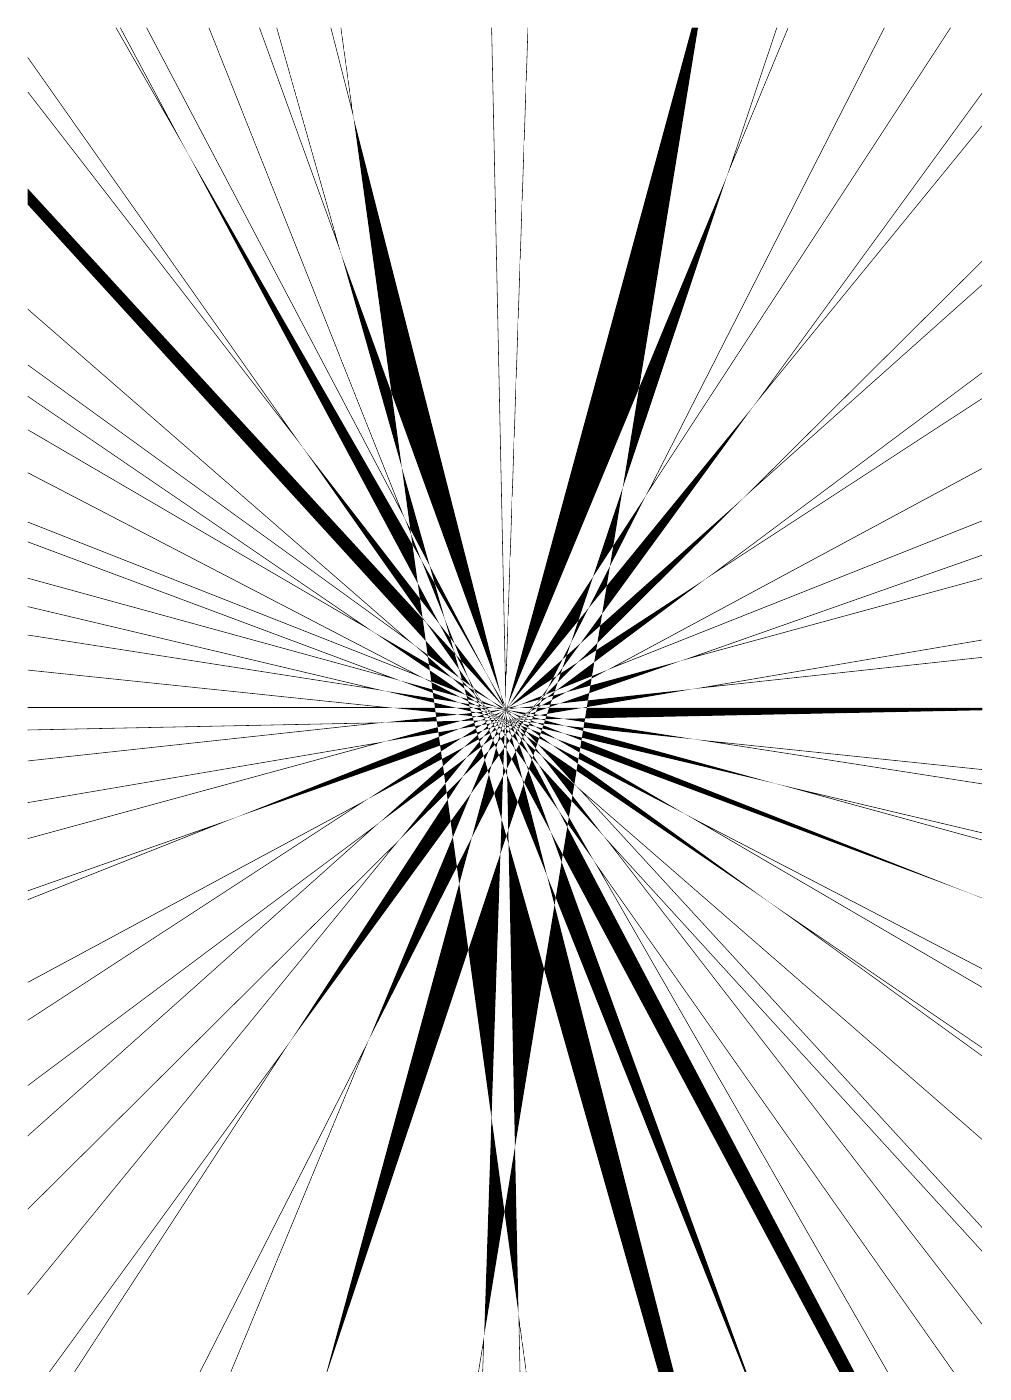
\begin{tikzpicture}[x=\linewidth,y=\linewidth]
\useasboundingbox (0,0) rectangle (1,1.40794);
\clip (0,0) rectangle (1,1.40794);
% External black cell outlines (inset)
\begin{scope}\clip (0.47187,0.00000) -- (0.47685,-0.00000) -- (0.47814,0.03830) -- cycle; \draw[line width=0.4pt] (0.47685,-0.00000) -- (0.47814,0.03830) (0.47814,0.03830) -- (0.47187,0.00000);\end{scope}
\begin{scope}\clip (0.52251,0.00000) -- (0.51407,0.06122) -- (0.51536,0.00000) -- cycle; \draw[line width=0.4pt] (0.52251,0.00000) -- (0.51407,0.06122) (0.51407,0.06122) -- (0.51536,0.00000);\end{scope}
\begin{scope}\clip (0.18019,0.00000) -- (0.21311,-0.00000) -- (0.35751,0.34827) -- cycle; \draw[line width=0.4pt] (0.21311,-0.00000) -- (0.35751,0.34827) (0.35751,0.34827) -- (0.18019,0.00000);\end{scope}
\begin{scope}\clip (0.97009,0.00000) -- (0.59296,0.53549) -- (0.90036,0.00000) -- cycle; \draw[line width=0.4pt] (0.97009,0.00000) -- (0.59296,0.53549) (0.59296,0.53549) -- (0.90036,0.00000);\end{scope}
\begin{scope}\clip (1.00000,0.12640) -- (0.60304,0.56162) -- (1.00000,0.04900) -- cycle; \draw[line width=0.4pt] (1.00000,0.12640) -- (0.60304,0.56162) (0.60304,0.56162) -- (1.00000,0.04900);\end{scope}
\begin{scope}\clip (1.00000,0.24355) -- (0.57463,0.61364) -- (1.00000,0.15039) -- cycle; \draw[line width=0.4pt] (1.00000,0.24355) -- (0.57463,0.61364) (0.57463,0.61364) -- (1.00000,0.15039);\end{scope}
\begin{scope}\clip (1.00000,0.33962) -- (0.77626,0.49235) -- (1.00000,0.33033) -- cycle; \draw[line width=0.4pt] (1.00000,0.33962) -- (0.77626,0.49235) (0.77626,0.49235) -- (1.00000,0.33033);\end{scope}
\begin{scope}\clip (1.00000,0.42243) -- (0.68803,0.58457) -- (1.00000,0.40230) -- cycle; \draw[line width=0.4pt] (1.00000,0.42243) -- (0.68803,0.58457) (0.68803,0.58457) -- (1.00000,0.40230);\end{scope}
\begin{scope}\clip (1.00000,0.49638) -- (0.98561,0.50175) -- (1.00000,0.49609) -- cycle; \draw[line width=0.4pt] (1.00000,0.49638) -- (0.98561,0.50175) (0.98561,0.50175) -- (1.00000,0.49609);\end{scope}
\begin{scope}\clip (1.00000,0.56480) -- (0.78329,0.61618) -- (1.00000,0.55673) -- cycle; \draw[line width=0.4pt] (1.00000,0.56480) -- (0.78329,0.61618) (0.78329,0.61618) -- (1.00000,0.55673);\end{scope}
\begin{scope}\clip (1.00000,0.63115) -- (0.69849,0.66258) -- (1.00000,0.61556) -- cycle; \draw[line width=0.4pt] (1.00000,0.63115) -- (0.69849,0.66258) (0.69849,0.66258) -- (1.00000,0.61556);\end{scope}
\begin{scope}\clip (1.00000,0.76694) -- (0.69627,0.71519) -- (1.00000,0.74815) -- cycle; \draw[line width=0.4pt] (1.00000,0.76694) -- (0.69627,0.71519) (0.69627,0.71519) -- (1.00000,0.74815);\end{scope}
\begin{scope}\clip (1.00000,0.85583) -- (0.68370,0.74458) -- (1.00000,0.83079) -- cycle; \draw[line width=0.4pt] (1.00000,0.85583) -- (0.68370,0.74458) (0.68370,0.74458) -- (1.00000,0.83079);\end{scope}
\begin{scope}\clip (1.00000,0.94672) -- (0.60737,0.73529) -- (1.00000,0.89114) -- cycle; \draw[line width=0.4pt] (1.00000,0.94672) -- (0.60737,0.73529) (0.60737,0.73529) -- (1.00000,0.89114);\end{scope}
\begin{scope}\clip (1.00000,1.04707) -- (0.70971,0.83026) -- (1.00000,1.01937) -- cycle; \draw[line width=0.4pt] (1.00000,1.04707) -- (0.70971,0.83026) (0.70971,0.83026) -- (1.00000,1.01937);\end{scope}
\begin{scope}\clip (1.00000,1.16414) -- (0.74844,0.91423) -- (1.00000,1.13858) -- cycle; \draw[line width=0.4pt] (1.00000,1.16414) -- (0.74844,0.91423) (0.74844,0.91423) -- (1.00000,1.13858);\end{scope}
\begin{scope}\clip (1.00000,1.34034) -- (0.76001,1.01128) -- (1.00000,1.30517) -- cycle; \draw[line width=0.4pt] (1.00000,1.34034) -- (0.76001,1.01128) (0.76001,1.01128) -- (1.00000,1.30517);\end{scope}
\begin{scope}\clip (0.02249,0.00000) -- (0.04939,-0.00000) -- (0.27550,0.34692) -- cycle; \draw[line width=0.4pt] (0.04939,-0.00000) -- (0.27550,0.34692) (0.27550,0.34692) -- (0.02249,0.00000);\end{scope}
\begin{scope}\clip (0.00000,0.08054) -- (0.38995,0.55809) -- (0.00000,0.17069) -- cycle; \draw[line width=0.4pt] (0.00000,0.08054) -- (0.38995,0.55809) (0.38995,0.55809) -- (0.00000,0.17069);\end{scope}
\begin{scope}\clip (0.00000,0.24673) -- (0.36875,0.57560) -- (0.00000,0.30018) -- cycle; \draw[line width=0.4pt] (0.00000,0.24673) -- (0.36875,0.57560) (0.36875,0.57560) -- (0.00000,0.30018);\end{scope}
\begin{scope}\clip (0.00000,0.36790) -- (0.35695,0.60044) -- (0.00000,0.40823) -- cycle; \draw[line width=0.4pt] (0.00000,0.36790) -- (0.35695,0.60044) (0.35695,0.60044) -- (0.00000,0.40823);\end{scope}
\begin{scope}\clip (0.00000,0.49421) -- (0.21930,0.58125) -- (0.00000,0.50413) -- cycle; \draw[line width=0.4pt] (0.00000,0.49421) -- (0.21930,0.58125) (0.21930,0.58125) -- (0.00000,0.50413);\end{scope}
\begin{scope}\clip (0.00000,0.55824) -- (0.37505,0.66046) -- (0.00000,0.59656) -- cycle; \draw[line width=0.4pt] (0.00000,0.55824) -- (0.37505,0.66046) (0.37505,0.66046) -- (0.00000,0.59656);\end{scope}
\begin{scope}\clip (-0.00000,0.63961) -- (0.37448,0.68026) -- (0.00000,0.67262) -- cycle; \draw[line width=0.4pt] (-0.00000,0.63961) -- (0.37448,0.68026) (0.37448,0.68026) -- (0.00000,0.67262);\end{scope}
\begin{scope}\clip (-0.00000,0.69559) -- (0.38182,0.69559) -- (0.00000,0.73539) -- cycle; \draw[line width=0.4pt] (-0.00000,0.69559) -- (0.38182,0.69559) (0.38182,0.69559) -- (0.00000,0.73539);\end{scope}
\begin{scope}\clip (0.00000,0.77152) -- (0.37426,0.71315) -- (0.00000,0.80188) -- cycle; \draw[line width=0.4pt] (0.00000,0.77152) -- (0.37426,0.71315) (0.37426,0.71315) -- (0.00000,0.80188);\end{scope}
\begin{scope}\clip (0.00000,0.83105) -- (0.39052,0.72392) -- (0.00000,0.86971) -- cycle; \draw[line width=0.4pt] (0.00000,0.83105) -- (0.39052,0.72392) (0.39052,0.72392) -- (0.00000,0.86971);\end{scope}
\begin{scope}\clip (0.00000,0.88986) -- (0.41517,0.72638) -- (-0.00000,0.94215) -- cycle; \draw[line width=0.4pt] (0.00000,0.88986) -- (0.41517,0.72638) (0.41517,0.72638) -- (-0.00000,0.94215);\end{scope}
\begin{scope}\clip (0.00000,0.98654) -- (0.36268,0.77465) -- (0.00000,1.02221) -- cycle; \draw[line width=0.4pt] (0.00000,0.98654) -- (0.36268,0.77465) (0.36268,0.77465) -- (0.00000,1.02221);\end{scope}
\begin{scope}\clip (-0.00000,1.05444) -- (0.40537,0.76091) -- (-0.00000,1.11360) -- cycle; \draw[line width=0.4pt] (-0.00000,1.05444) -- (0.40537,0.76091) (0.40537,0.76091) -- (-0.00000,1.11360);\end{scope}
\begin{scope}\clip (0.00000,1.34034) -- (0.28845,0.96785) -- (0.00000,1.37742) -- cycle; \draw[line width=0.4pt] (0.00000,1.34034) -- (0.28845,0.96785) (0.28845,0.96785) -- (0.00000,1.37742);\end{scope}
\begin{scope}\clip (0.09212,1.40794) -- (0.16790,1.27593) -- (0.09731,1.40794) -- cycle; \draw[line width=0.4pt] (0.09212,1.40794) -- (0.16790,1.27593) (0.16790,1.27593) -- (0.09731,1.40794);\end{scope}
\begin{scope}\clip (0.12417,1.40794) -- (0.39483,0.89408) -- (0.19013,1.40794) -- cycle; \draw[line width=0.4pt] (0.12417,1.40794) -- (0.39483,0.89408) (0.39483,0.89408) -- (0.19013,1.40794);\end{scope}
\begin{scope}\clip (0.24245,1.40794) -- (0.32843,1.17076) -- (0.26113,1.40794) -- cycle; \draw[line width=0.4pt] (0.24245,1.40794) -- (0.32843,1.17076) (0.32843,1.17076) -- (0.26113,1.40794);\end{scope}
\begin{scope}\clip (0.31725,1.40794) -- (0.34137,1.31346) -- (0.32834,1.40794) -- cycle; \draw[line width=0.4pt] (0.31725,1.40794) -- (0.34137,1.31346) (0.34137,1.31346) -- (0.32834,1.40794);\end{scope}
\begin{scope}\clip (0.89702,1.40794) -- (0.64712,0.91711) -- (0.96703,1.40794) -- cycle; \draw[line width=0.4pt] (0.89702,1.40794) -- (0.64712,0.91711) (0.64712,0.91711) -- (0.96703,1.40794);\end{scope}
\begin{scope}\clip (0.78437,1.40794) -- (0.73238,1.25240) -- (0.79687,1.40794) -- cycle; \draw[line width=0.4pt] (0.78437,1.40794) -- (0.73238,1.25240) (0.73238,1.25240) -- (0.79687,1.40794);\end{scope}
\begin{scope}\clip (0.48564,1.40794) -- (0.50053,0.70271) -- (0.52430,1.40794) -- cycle; \draw[line width=0.4pt] (0.48564,1.40794) -- (0.50053,0.70271) (0.50053,0.70271) -- (0.52430,1.40794);\end{scope}
% Filled cells
\fill (0.47814,0.03830) -- (0.49934,0.16800) -- (0.48581,0.26609) -- cycle;
\fill (0.31311,0.00000) -- (0.31374,0.00000) -- (0.46153,0.44215) -- (0.45201,0.51120) -- cycle;
\fill (0.35751,0.34827) -- (0.44955,0.52905) -- (0.44528,0.55997) -- cycle;
\fill (0.27550,0.34692) -- (0.44299,0.57658) -- (0.43988,0.59913) -- cycle;
\fill (0.49934,0.16800) -- (0.51407,0.06122) -- (0.51039,0.23556) -- cycle;
\fill (0.46153,0.44215) -- (0.48581,0.26609) -- (0.49514,0.54267) -- cycle;
\fill (0.50369,0.55307) -- (0.51039,0.23556) -- (0.54088,0.42201) -- cycle;
\fill (0.49514,0.54267) -- (0.50136,0.56128) -- (0.49636,0.57891) -- cycle;
\fill (0.44955,0.52905) -- (0.45201,0.51120) -- (0.46522,0.55983) -- cycle;
\fill (0.46522,0.55983) -- (0.48869,0.60593) -- (0.48310,0.62563) -- cycle;
\fill (0.44299,0.57658) -- (0.44528,0.55997) -- (0.46427,0.60576) -- cycle;
\fill (0.46427,0.60576) -- (0.48189,0.62991) -- (0.47880,0.64080) -- cycle;
\fill (0.45570,0.62340) -- (0.47757,0.64513) -- (0.47523,0.65337) -- cycle;
\fill (0.54088,0.42201) -- (0.66061,0.00000) -- (0.67665,0.00000) -- (0.55183,0.48899) -- cycle;
\fill (0.50136,0.56128) -- (0.50369,0.55307) -- (0.50339,0.56735) -- cycle;
\fill (0.54402,0.51957) -- (0.55183,0.48899) -- (0.55310,0.49678) -- cycle;
\fill (0.48869,0.60593) -- (0.49636,0.57891) -- (0.49787,0.62396) -- cycle;
\fill (0.50218,0.62461) -- (0.50339,0.56735) -- (0.51324,0.59683) -- cycle;
\fill (0.49787,0.62396) -- (0.50043,0.62899) -- (0.49823,0.63452) -- cycle;
\fill (0.48189,0.62991) -- (0.48310,0.62563) -- (0.48568,0.63511) -- cycle;
\fill (0.48568,0.63511) -- (0.49364,0.64603) -- (0.49067,0.65349) -- cycle;
\fill (0.47757,0.64513) -- (0.47880,0.64080) -- (0.48271,0.65024) -- cycle;
\fill (0.48271,0.65024) -- (0.48934,0.65683) -- (0.48743,0.66162) -- cycle;
\fill (0.47746,0.65679) -- (0.48663,0.66364) -- (0.48484,0.66812) -- cycle;
\fill (0.55310,0.49678) -- (0.75099,0.00000) -- (0.75283,0.00000) -- (0.55921,0.53413) -- cycle;
\fill (0.51324,0.59683) -- (0.54402,0.51957) -- (0.51951,0.61559) -- cycle;
\fill (0.54794,0.56521) -- (0.55921,0.53413) -- (0.56046,0.54180) -- cycle;
\fill (0.50043,0.62899) -- (0.50218,0.62461) -- (0.50202,0.63210) -- cycle;
\fill (0.51815,0.62093) -- (0.51951,0.61559) -- (0.52008,0.61731) -- cycle;
\fill (0.49364,0.64603) -- (0.49823,0.63452) -- (0.49886,0.65319) -- cycle;
\fill (0.50160,0.65187) -- (0.50202,0.63210) -- (0.50697,0.64183) -- cycle;
\fill (0.49886,0.65319) -- (0.50004,0.65480) -- (0.49898,0.65677) -- cycle;
\fill (0.48934,0.65683) -- (0.49067,0.65349) -- (0.49240,0.65987) -- cycle;
\fill (0.49240,0.65987) -- (0.49562,0.66306) -- (0.49406,0.66597) -- cycle;
\fill (0.48663,0.66364) -- (0.48743,0.66162) -- (0.48900,0.66541) -- cycle;
\fill (0.48900,0.66541) -- (0.49283,0.66827) -- (0.49134,0.67106) -- cycle;
\fill (0.48604,0.66996) -- (0.49061,0.67242) -- (0.48928,0.67492) -- cycle;
\fill (0.56046,0.54180) -- (0.85018,0.00000) -- (0.86578,0.00000) -- (0.56518,0.57067) -- cycle;
\fill (0.52008,0.61731) -- (0.54794,0.56521) -- (0.52439,0.63018) -- cycle;
\fill (0.55629,0.58755) -- (0.56518,0.57067) -- (0.56575,0.57412) -- cycle;
\fill (0.50697,0.64183) -- (0.51815,0.62093) -- (0.51086,0.64947) -- cycle;
\fill (0.52240,0.63568) -- (0.52439,0.63018) -- (0.52499,0.63199) -- cycle;
\fill (0.50004,0.65480) -- (0.50160,0.65187) -- (0.50150,0.65681) -- cycle;
\fill (0.50983,0.65353) -- (0.51086,0.64947) -- (0.51163,0.65097) -- cycle;
\fill (0.49562,0.66306) -- (0.49898,0.65677) -- (0.49932,0.66673) -- cycle;
\fill (0.50131,0.66562) -- (0.50150,0.65681) -- (0.50456,0.66100) -- cycle;
\fill (0.49932,0.66673) -- (0.50003,0.66744) -- (0.49937,0.66837) -- cycle;
\fill (0.49283,0.66827) -- (0.49406,0.66597) -- (0.49516,0.67001) -- cycle;
\fill (0.49516,0.67001) -- (0.49716,0.67151) -- (0.49601,0.67314) -- cycle;
\fill (0.49061,0.67242) -- (0.49134,0.67106) -- (0.49228,0.67332) -- cycle;
\fill (0.49228,0.67332) -- (0.49490,0.67472) -- (0.49362,0.67654) -- cycle;
\fill (0.49036,0.67659) -- (0.49295,0.67750) -- (0.49191,0.67896) -- cycle;
\fill (0.56575,0.57412) -- (0.59296,0.53549) -- (0.56686,0.58094) -- cycle;
\fill (0.52499,0.63199) -- (0.55629,0.58755) -- (0.52806,0.64116) -- cycle;
\fill (0.53537,0.63581) -- (0.56686,0.58094) -- (0.56968,0.59819) -- cycle;
\fill (0.51163,0.65097) -- (0.52240,0.63568) -- (0.51468,0.65697) -- cycle;
\fill (0.52473,0.64747) -- (0.52806,0.64116) -- (0.52871,0.64311) -- cycle;
\fill (0.50456,0.66100) -- (0.50983,0.65353) -- (0.50705,0.66441) -- cycle;
\fill (0.51376,0.65949) -- (0.51468,0.65697) -- (0.51518,0.65794) -- cycle;
\fill (0.50003,0.66744) -- (0.50131,0.66562) -- (0.50125,0.66865) -- cycle;
\fill (0.50618,0.66781) -- (0.50705,0.66441) -- (0.50804,0.66577) -- cycle;
\fill (0.49716,0.67151) -- (0.49937,0.66837) -- (0.49954,0.67328) -- cycle;
\fill (0.50115,0.67332) -- (0.50125,0.66865) -- (0.50343,0.67082) -- cycle;
\fill (0.49954,0.67328) -- (0.50052,0.67401) -- (0.49960,0.67503) -- cycle;
\fill (0.49490,0.67472) -- (0.49601,0.67314) -- (0.49671,0.67570) -- cycle;
\fill (0.49671,0.67570) -- (0.49823,0.67652) -- (0.49723,0.67762) -- cycle;
\fill (0.49295,0.67750) -- (0.49362,0.67654) -- (0.49419,0.67793) -- cycle;
\fill (0.49419,0.67793) -- (0.49628,0.67867) -- (0.49505,0.68001) -- cycle;
\fill (0.49294,0.68055) -- (0.49434,0.68078) -- (0.49362,0.68158) -- cycle;
\fill (0.56968,0.59819) -- (0.60304,0.56162) -- (0.57056,0.60356) -- cycle;
\fill (0.52871,0.64311) -- (0.53537,0.63581) -- (0.52962,0.64582) -- cycle;
\fill (0.53821,0.64534) -- (0.57056,0.60356) -- (0.57251,0.61549) -- cycle;
\fill (0.51518,0.65794) -- (0.52473,0.64747) -- (0.51716,0.66184) -- cycle;
\fill (0.52161,0.65978) -- (0.52962,0.64582) -- (0.53143,0.65123) -- cycle;
\fill (0.50804,0.66577) -- (0.51376,0.65949) -- (0.51034,0.66893) -- cycle;
\fill (0.51541,0.66517) -- (0.51716,0.66184) -- (0.51780,0.66309) -- cycle;
\fill (0.50343,0.67082) -- (0.50618,0.66781) -- (0.50501,0.67239) -- cycle;
\fill (0.51000,0.66988) -- (0.51034,0.66893) -- (0.51063,0.66933) -- cycle;
\fill (0.50052,0.67401) -- (0.50115,0.67332) -- (0.50112,0.67447) -- cycle;
\fill (0.50441,0.67474) -- (0.50501,0.67239) -- (0.50599,0.67336) -- cycle;
\fill (0.49823,0.67652) -- (0.49960,0.67503) -- (0.49967,0.67730) -- cycle;
\fill (0.50106,0.67766) -- (0.50112,0.67447) -- (0.50306,0.67591) -- cycle;
\fill (0.49967,0.67730) -- (0.50078,0.67790) -- (0.49972,0.67882) -- cycle;
\fill (0.49628,0.67867) -- (0.49723,0.67762) -- (0.49764,0.67915) -- cycle;
\fill (0.49764,0.67915) -- (0.49885,0.67957) -- (0.49797,0.68034) -- cycle;
\fill (0.49434,0.68078) -- (0.49505,0.68001) -- (0.49545,0.68097) -- cycle;
\fill (0.49545,0.68097) -- (0.49695,0.68123) -- (0.49593,0.68212) -- cycle;
\fill (0.49435,0.68271) -- (0.49523,0.68272) -- (0.49468,0.68321) -- cycle;
\fill (0.57251,0.61549) -- (0.57463,0.61364) -- (0.57258,0.61588) -- cycle;
\fill (0.53143,0.65123) -- (0.53821,0.64534) -- (0.53209,0.65323) -- cycle;
\fill (0.53446,0.65740) -- (0.57258,0.61588) -- (0.57485,0.62982) -- cycle;
\fill (0.51780,0.66309) -- (0.52161,0.65978) -- (0.51869,0.66485) -- cycle;
\fill (0.52260,0.66549) -- (0.53209,0.65323) -- (0.53367,0.65794) -- cycle;
\fill (0.51063,0.66933) -- (0.51541,0.66517) -- (0.51213,0.67139) -- cycle;
\fill (0.51558,0.67029) -- (0.51869,0.66485) -- (0.51994,0.66730) -- cycle;
\fill (0.50599,0.67336) -- (0.51000,0.66988) -- (0.50801,0.67537) -- cycle;
\fill (0.51111,0.67334) -- (0.51213,0.67139) -- (0.51274,0.67222) -- cycle;
\fill (0.50306,0.67591) -- (0.50441,0.67474) -- (0.50394,0.67657) -- cycle;
\fill (0.50797,0.67548) -- (0.50801,0.67537) -- (0.50806,0.67542) -- cycle;
\fill (0.50078,0.67790) -- (0.50106,0.67766) -- (0.50105,0.67804) -- cycle;
\fill (0.50343,0.67857) -- (0.50394,0.67657) -- (0.50510,0.67744) -- cycle;
\fill (0.49885,0.67957) -- (0.49972,0.67882) -- (0.49976,0.67989) -- cycle;
\fill (0.50100,0.68023) -- (0.50105,0.67804) -- (0.50282,0.67899) -- cycle;
\fill (0.49976,0.67989) -- (0.50091,0.68030) -- (0.49980,0.68105) -- cycle;
\fill (0.49695,0.68123) -- (0.49797,0.68034) -- (0.49827,0.68145) -- cycle;
\fill (0.49827,0.68145) -- (0.49903,0.68158) -- (0.49842,0.68200) -- cycle;
\fill (0.49523,0.68272) -- (0.49593,0.68212) -- (0.49619,0.68274) -- cycle;
\fill (0.49619,0.68274) -- (0.49729,0.68277) -- (0.49644,0.68335) -- cycle;
\fill (0.49506,0.68379) -- (0.49593,0.68370) -- (0.49528,0.68414) -- cycle;
\fill (0.57485,0.62982) -- (0.77626,0.49235) -- (0.57608,0.63730) -- cycle;
\fill (0.53367,0.65794) -- (0.53446,0.65740) -- (0.53375,0.65817) -- cycle;
\fill (0.54940,0.65662) -- (0.57608,0.63730) -- (0.57690,0.64232) -- cycle;
\fill (0.51994,0.66730) -- (0.52260,0.66549) -- (0.52044,0.66828) -- cycle;
\fill (0.52219,0.67076) -- (0.53375,0.65817) -- (0.53562,0.66378) -- cycle;
\fill (0.51274,0.67222) -- (0.51558,0.67029) -- (0.51371,0.67354) -- cycle;
\fill (0.51605,0.67395) -- (0.52044,0.66828) -- (0.52180,0.67096) -- cycle;
\fill (0.50806,0.67542) -- (0.51111,0.67334) -- (0.50934,0.67669) -- cycle;
\fill (0.51238,0.67586) -- (0.51371,0.67354) -- (0.51456,0.67472) -- cycle;
\fill (0.50510,0.67744) -- (0.50797,0.67548) -- (0.50680,0.67871) -- cycle;
\fill (0.50880,0.67772) -- (0.50934,0.67669) -- (0.50983,0.67718) -- cycle;
\fill (0.50282,0.67899) -- (0.50343,0.67857) -- (0.50326,0.67923) -- cycle;
\fill (0.50678,0.67877) -- (0.50680,0.67871) -- (0.50684,0.67874) -- cycle;
\fill (0.50091,0.68030) -- (0.50100,0.68023) -- (0.50100,0.68033) -- cycle;
\fill (0.50286,0.68080) -- (0.50326,0.67923) -- (0.50455,0.67992) -- cycle;
\fill (0.49903,0.68158) -- (0.49980,0.68105) -- (0.49982,0.68172) -- cycle;
\fill (0.50097,0.68179) -- (0.50100,0.68033) -- (0.50266,0.68091) -- cycle;
\fill (0.49982,0.68172) -- (0.50079,0.68188) -- (0.49984,0.68237) -- cycle;
\fill (0.49729,0.68277) -- (0.49842,0.68200) -- (0.49863,0.68279) -- cycle;
\fill (0.49863,0.68279) -- (0.49902,0.68280) -- (0.49868,0.68297) -- cycle;
\fill (0.49593,0.68370) -- (0.49644,0.68335) -- (0.49656,0.68363) -- cycle;
\fill (0.49656,0.68363) -- (0.49763,0.68352) -- (0.49671,0.68400) -- cycle;
\fill (0.49547,0.68442) -- (0.49628,0.68422) -- (0.49558,0.68459) -- cycle;
\fill (0.57690,0.64232) -- (0.68803,0.58457) -- (0.57797,0.64887) -- cycle;
\fill (0.57875,0.65365) -- (0.98561,0.50175) -- (0.58003,0.66146) -- cycle;
\fill (0.53562,0.66378) -- (0.54940,0.65662) -- (0.53638,0.66605) -- cycle;
\fill (0.53739,0.66909) -- (0.55393,0.66291) -- (0.53837,0.67201) -- cycle;
\fill (0.52180,0.67096) -- (0.52219,0.67076) -- (0.52187,0.67110) -- cycle;
\fill (0.52349,0.67428) -- (0.52662,0.67311) -- (0.52390,0.67508) -- cycle;
\fill (0.51456,0.67472) -- (0.51605,0.67395) -- (0.51499,0.67531) -- cycle;
\fill (0.51622,0.67699) -- (0.51659,0.67685) -- (0.51633,0.67714) -- cycle;
\fill (0.50983,0.67718) -- (0.51238,0.67586) -- (0.51097,0.67831) -- cycle;
\fill (0.51144,0.67878) -- (0.51266,0.67832) -- (0.51193,0.67927) -- cycle;
\fill (0.50684,0.67874) -- (0.50880,0.67772) -- (0.50786,0.67950) -- cycle;
\fill (0.50841,0.67991) -- (0.51050,0.67913) -- (0.50956,0.68077) -- cycle;
\fill (0.50455,0.67992) -- (0.50678,0.67877) -- (0.50606,0.68074) -- cycle;
\fill (0.50611,0.68077) -- (0.50746,0.68026) -- (0.50695,0.68122) -- cycle;
\fill (0.50266,0.68091) -- (0.50286,0.68080) -- (0.50282,0.68097) -- cycle;
\fill (0.50424,0.68147) -- (0.50604,0.68079) -- (0.50562,0.68195) -- cycle;
\fill (0.50079,0.68188) -- (0.50097,0.68179) -- (0.50097,0.68191) -- cycle;
\fill (0.50239,0.68216) -- (0.50253,0.68210) -- (0.50251,0.68218) -- cycle;
\fill (0.50058,0.68283) -- (0.50095,0.68269) -- (0.50095,0.68284) -- cycle;
\fill (0.49902,0.68280) -- (0.49984,0.68237) -- (0.49986,0.68282) -- cycle;
\fill (0.49986,0.68282) -- (0.50058,0.68283) -- (0.49987,0.68310) -- cycle;
\fill (0.50050,0.68322) -- (0.50094,0.68312) -- (0.50094,0.68318) -- cycle;
\fill (0.49987,0.68329) -- (0.50050,0.68322) -- (0.49988,0.68337) -- cycle;
\fill (0.50003,0.68794) -- (0.50055,0.68986) -- (0.50015,0.69144) -- cycle;
\fill (0.49916,0.68336) -- (0.49987,0.68310) -- (0.49987,0.68329) -- cycle;
\fill (0.49763,0.68352) -- (0.49868,0.68297) -- (0.49880,0.68340) -- cycle;
\fill (0.49880,0.68340) -- (0.49916,0.68336) -- (0.49882,0.68349) -- cycle;
\fill (0.49886,0.68361) -- (0.49988,0.68337) -- (0.50003,0.68794) -- cycle;
\fill (0.49786,0.68385) -- (0.49882,0.68349) -- (0.49886,0.68361) -- cycle;
\fill (0.49628,0.68422) -- (0.49671,0.68400) -- (0.49676,0.68411) -- cycle;
\fill (0.49676,0.68411) -- (0.49786,0.68385) -- (0.49681,0.68424) -- cycle;
\fill (0.49564,0.68468) -- (0.49681,0.68424) -- (0.49936,0.69039) -- cycle;
\fill (0.50095,0.68269) -- (0.50097,0.68191) -- (0.50239,0.68216) -- cycle;
\fill (0.50202,0.68286) -- (0.50236,0.68278) -- (0.50234,0.68287) -- cycle;
\fill (0.50094,0.68312) -- (0.50095,0.68284) -- (0.50202,0.68286) -- cycle;
\fill (0.50082,0.68880) -- (0.50094,0.68318) -- (0.50229,0.68303) -- cycle;
\fill (0.50253,0.68210) -- (0.50282,0.68097) -- (0.50424,0.68147) -- cycle;
\fill (0.50391,0.68241) -- (0.50560,0.68201) -- (0.50537,0.68266) -- cycle;
\fill (0.50055,0.68986) -- (0.50082,0.68880) -- (0.50078,0.69070) -- cycle;
\fill (0.50012,0.69156) -- (0.50015,0.69144) -- (0.50015,0.69161) -- cycle;
\fill (0.50236,0.68278) -- (0.50251,0.68218) -- (0.50391,0.68241) -- cycle;
\fill (0.50364,0.68289) -- (0.50535,0.68272) -- (0.50527,0.68293) -- cycle;
\fill (0.50229,0.68303) -- (0.50234,0.68287) -- (0.50364,0.68289) -- cycle;
\fill (0.50076,0.69184) -- (0.50078,0.69070) -- (0.50104,0.69164) -- cycle;
\fill (0.50604,0.68079) -- (0.50606,0.68074) -- (0.50611,0.68077) -- cycle;
\fill (0.50571,0.68199) -- (0.50667,0.68176) -- (0.50642,0.68223) -- cycle;
\fill (0.50560,0.68201) -- (0.50562,0.68195) -- (0.50571,0.68199) -- cycle;
\fill (0.50556,0.68269) -- (0.50621,0.68263) -- (0.50613,0.68279) -- cycle;
\fill (0.50535,0.68272) -- (0.50537,0.68266) -- (0.50556,0.68269) -- cycle;
\fill (0.50354,0.68771) -- (0.50527,0.68293) -- (0.50605,0.68294) -- cycle;
\fill (0.50746,0.68026) -- (0.50786,0.67950) -- (0.50841,0.67991) -- cycle;
\fill (0.50756,0.68155) -- (0.50935,0.68112) -- (0.50875,0.68218) -- cycle;
\fill (0.50173,0.69113) -- (0.50354,0.68771) -- (0.50249,0.69058) -- cycle;
\fill (0.50667,0.68176) -- (0.50695,0.68122) -- (0.50756,0.68155) -- cycle;
\fill (0.50723,0.68252) -- (0.50864,0.68237) -- (0.50833,0.68291) -- cycle;
\fill (0.50621,0.68263) -- (0.50642,0.68223) -- (0.50723,0.68252) -- cycle;
\fill (0.50715,0.68297) -- (0.50828,0.68299) -- (0.50819,0.68314) -- cycle;
\fill (0.50605,0.68294) -- (0.50613,0.68279) -- (0.50715,0.68297) -- cycle;
\fill (0.51050,0.67913) -- (0.51097,0.67831) -- (0.51144,0.67878) -- cycle;
\fill (0.50987,0.68100) -- (0.51075,0.68079) -- (0.51033,0.68134) -- cycle;
\fill (0.50935,0.68112) -- (0.50956,0.68077) -- (0.50987,0.68100) -- cycle;
\fill (0.50903,0.68233) -- (0.50960,0.68227) -- (0.50940,0.68253) -- cycle;
\fill (0.50864,0.68237) -- (0.50875,0.68218) -- (0.50903,0.68233) -- cycle;
\fill (0.50858,0.68300) -- (0.50904,0.68300) -- (0.50894,0.68312) -- cycle;
\fill (0.50828,0.68299) -- (0.50833,0.68291) -- (0.50858,0.68300) -- cycle;
\fill (0.50609,0.68681) -- (0.50819,0.68314) -- (0.50884,0.68325) -- cycle;
\fill (0.51266,0.67832) -- (0.51499,0.67531) -- (0.51622,0.67699) -- cycle;
\fill (0.51294,0.68027) -- (0.51359,0.68012) -- (0.51321,0.68054) -- cycle;
\fill (0.50403,0.68947) -- (0.50609,0.68681) -- (0.50494,0.68881) -- cycle;
\fill (0.51075,0.68079) -- (0.51193,0.67927) -- (0.51294,0.68027) -- cycle;
\fill (0.51133,0.68209) -- (0.51183,0.68204) -- (0.51160,0.68229) -- cycle;
\fill (0.50960,0.68227) -- (0.51033,0.68134) -- (0.51133,0.68209) -- cycle;
\fill (0.51032,0.68303) -- (0.51091,0.68304) -- (0.51072,0.68325) -- cycle;
\fill (0.50904,0.68300) -- (0.50940,0.68253) -- (0.51032,0.68303) -- cycle;
\fill (0.50977,0.68341) -- (0.51046,0.68353) -- (0.51037,0.68362) -- cycle;
\fill (0.50884,0.68325) -- (0.50894,0.68312) -- (0.50977,0.68341) -- cycle;
\fill (0.51659,0.67685) -- (0.52187,0.67110) -- (0.52349,0.67428) -- cycle;
\fill (0.51778,0.67913) -- (0.51858,0.67894) -- (0.51796,0.67938) -- cycle;
\fill (0.51359,0.68012) -- (0.51633,0.67714) -- (0.51778,0.67913) -- cycle;
\fill (0.51445,0.68177) -- (0.51470,0.68174) -- (0.51454,0.68186) -- cycle;
\fill (0.51183,0.68204) -- (0.51321,0.68054) -- (0.51445,0.68177) -- cycle;
\fill (0.51265,0.68308) -- (0.51285,0.68308) -- (0.51275,0.68315) -- cycle;
\fill (0.51091,0.68304) -- (0.51160,0.68229) -- (0.51265,0.68308) -- cycle;
\fill (0.51161,0.68373) -- (0.51189,0.68377) -- (0.51181,0.68383) -- cycle;
\fill (0.51046,0.68353) -- (0.51072,0.68325) -- (0.51161,0.68373) -- cycle;
\fill (0.50695,0.68736) -- (0.51037,0.68362) -- (0.51154,0.68403) -- cycle;
\fill (0.52662,0.67311) -- (0.53638,0.66605) -- (0.53739,0.66909) -- cycle;
\fill (0.52508,0.67739) -- (0.53192,0.67577) -- (0.52601,0.67923) -- cycle;
\fill (0.50045,0.69206) -- (0.50076,0.69184) -- (0.50074,0.69251) -- cycle;
\fill (0.50104,0.69164) -- (0.50173,0.69113) -- (0.50118,0.69218) -- cycle;
\fill (0.50096,0.69260) -- (0.50118,0.69218) -- (0.50126,0.69248) -- cycle;
\fill (0.50190,0.69222) -- (0.50249,0.69058) -- (0.50403,0.68947) -- cycle;
\fill (0.50189,0.69223) -- (0.50190,0.69222) -- (0.50190,0.69223) -- cycle;
\fill (0.50382,0.69076) -- (0.50494,0.68881) -- (0.50695,0.68736) -- cycle;
\fill (0.51858,0.67894) -- (0.52390,0.67508) -- (0.52508,0.67739) -- cycle;
\fill (0.51933,0.68126) -- (0.52323,0.68085) -- (0.52029,0.68257) -- cycle;
\fill (0.51470,0.68174) -- (0.51796,0.67938) -- (0.51933,0.68126) -- cycle;
\fill (0.51583,0.68314) -- (0.51919,0.68321) -- (0.51712,0.68442) -- cycle;
\fill (0.50280,0.69187) -- (0.50382,0.69076) -- (0.50330,0.69168) -- cycle;
\fill (0.51285,0.68308) -- (0.51454,0.68186) -- (0.51583,0.68314) -- cycle;
\fill (0.51409,0.68415) -- (0.51680,0.68461) -- (0.51562,0.68530) -- cycle;
\fill (0.51189,0.68377) -- (0.51275,0.68315) -- (0.51409,0.68415) -- cycle;
\fill (0.51340,0.68469) -- (0.51544,0.68540) -- (0.51510,0.68560) -- cycle;
\fill (0.51154,0.68403) -- (0.51181,0.68383) -- (0.51340,0.68469) -- cycle;
\fill (0.55393,0.66291) -- (0.57797,0.64887) -- (0.57875,0.65365) -- cycle;
\fill (0.53906,0.67408) -- (0.56149,0.66876) -- (0.54010,0.67718) -- cycle;
\fill (0.53192,0.67577) -- (0.53837,0.67201) -- (0.53906,0.67408) -- cycle;
\fill (0.52666,0.68050) -- (0.53350,0.67978) -- (0.52750,0.68215) -- cycle;
\fill (0.52323,0.68085) -- (0.52601,0.67923) -- (0.52666,0.68050) -- cycle;
\fill (0.52078,0.68324) -- (0.52452,0.68332) -- (0.52166,0.68445) -- cycle;
\fill (0.51919,0.68321) -- (0.52029,0.68257) -- (0.52078,0.68324) -- cycle;
\fill (0.51742,0.68471) -- (0.51990,0.68514) -- (0.51843,0.68572) -- cycle;
\fill (0.51680,0.68461) -- (0.51712,0.68442) -- (0.51742,0.68471) -- cycle;
\fill (0.51607,0.68563) -- (0.51744,0.68611) -- (0.51696,0.68630) -- cycle;
\fill (0.51544,0.68540) -- (0.51562,0.68530) -- (0.51607,0.68563) -- cycle;
\fill (0.50760,0.68998) -- (0.51510,0.68560) -- (0.51663,0.68643) -- cycle;
\fill (0.58048,0.66426) -- (0.78329,0.61618) -- (0.58167,0.67149) -- cycle;
\fill (0.50083,0.69265) -- (0.50096,0.69260) -- (0.50089,0.69274) -- cycle;
\fill (0.50126,0.69248) -- (0.50189,0.69223) -- (0.50138,0.69289) -- cycle;
\fill (0.50118,0.69314) -- (0.50138,0.69289) -- (0.50148,0.69326) -- cycle;
\fill (0.50152,0.69327) -- (0.50190,0.69223) -- (0.50280,0.69187) -- cycle;
\fill (0.50151,0.69327) -- (0.50152,0.69327) -- (0.50152,0.69327) -- cycle;
\fill (0.50259,0.69291) -- (0.50330,0.69168) -- (0.50760,0.68998) -- cycle;
\fill (0.56149,0.66876) -- (0.58003,0.66146) -- (0.58048,0.66426) -- cycle;
\fill (0.54072,0.67903) -- (0.56241,0.67677) -- (0.54185,0.68241) -- cycle;
\fill (0.53350,0.67978) -- (0.54010,0.67718) -- (0.54072,0.67903) -- cycle;
\fill (0.52813,0.68339) -- (0.53756,0.68359) -- (0.52937,0.68583) -- cycle;
\fill (0.52452,0.68332) -- (0.52750,0.68215) -- (0.52813,0.68339) -- cycle;
\fill (0.52248,0.68558) -- (0.52730,0.68640) -- (0.52378,0.68736) -- cycle;
\fill (0.51990,0.68514) -- (0.52166,0.68445) -- (0.52248,0.68558) -- cycle;
\fill (0.51958,0.68686) -- (0.52222,0.68779) -- (0.52088,0.68816) -- cycle;
\fill (0.50206,0.69322) -- (0.50259,0.69291) -- (0.50244,0.69316) -- cycle;
\fill (0.51744,0.68611) -- (0.51843,0.68572) -- (0.51958,0.68686) -- cycle;
\fill (0.51846,0.68741) -- (0.52020,0.68835) -- (0.51984,0.68845) -- cycle;
\fill (0.51663,0.68643) -- (0.51696,0.68630) -- (0.51846,0.68741) -- cycle;
\fill (0.58219,0.67471) -- (0.69849,0.66258) -- (0.58315,0.68057) -- cycle;
\fill (0.56241,0.67677) -- (0.58167,0.67149) -- (0.58219,0.67471) -- cycle;
\fill (0.54227,0.68368) -- (0.56079,0.68406) -- (0.54331,0.68679) -- cycle;
\fill (0.53756,0.68359) -- (0.54185,0.68241) -- (0.54227,0.68368) -- cycle;
\fill (0.52989,0.68684) -- (0.53614,0.68790) -- (0.53085,0.68873) -- cycle;
\fill (0.52730,0.68640) -- (0.52937,0.68583) -- (0.52989,0.68684) -- cycle;
\fill (0.52474,0.68868) -- (0.52672,0.68937) -- (0.52540,0.68958) -- cycle;
\fill (0.52222,0.68779) -- (0.52378,0.68736) -- (0.52474,0.68868) -- cycle;
\fill (0.52211,0.68938) -- (0.52314,0.68993) -- (0.52273,0.69000) -- cycle;
\fill (0.52020,0.68835) -- (0.52088,0.68816) -- (0.52211,0.68938) -- cycle;
\fill (0.50294,0.69308) -- (0.51984,0.68845) -- (0.52206,0.69010) -- cycle;
\fill (0.50157,0.69330) -- (0.50206,0.69322) -- (0.50178,0.69338) -- cycle;
\fill (0.50240,0.69323) -- (0.50244,0.69316) -- (0.50294,0.69308) -- cycle;
\fill (0.58380,0.68453) -- (1.00000,0.69302) -- (1.00000,0.69559) -- (0.58561,0.69559) -- cycle;
\fill (0.56079,0.68406) -- (0.58315,0.68057) -- (0.58380,0.68453) -- cycle;
\fill (0.54414,0.68927) -- (0.58126,0.69559) -- (0.54625,0.69559) -- cycle;
\fill (0.53614,0.68790) -- (0.54331,0.68679) -- (0.54414,0.68927) -- cycle;
\fill (0.53215,0.69128) -- (0.54440,0.69559) -- (0.53434,0.69559) -- cycle;
\fill (0.52672,0.68937) -- (0.53085,0.68873) -- (0.53215,0.69128) -- cycle;
\fill (0.52729,0.69217) -- (0.53365,0.69559) -- (0.52979,0.69559) -- cycle;
\fill (0.52314,0.68993) -- (0.52540,0.68958) -- (0.52729,0.69217) -- cycle;
\fill (0.52520,0.69245) -- (0.52941,0.69559) -- (0.52837,0.69559) -- cycle;
\fill (0.50181,0.69339) -- (0.50240,0.69323) -- (0.50222,0.69355) -- cycle;
\fill (0.52206,0.69010) -- (0.52273,0.69000) -- (0.52520,0.69245) -- cycle;
\fill (0.58573,0.69635) -- (0.69627,0.71519) -- (0.58687,0.70331) -- cycle;
\fill (0.58126,0.69559) -- (0.58561,0.69559) -- (0.58573,0.69635) -- cycle;
\fill (0.54650,0.69633) -- (0.55720,0.70009) -- (0.54740,0.69903) -- cycle;
\fill (0.54440,0.69559) -- (0.54625,0.69559) -- (0.54650,0.69633) -- cycle;
\fill (0.53461,0.69611) -- (0.53817,0.69803) -- (0.53543,0.69773) -- cycle;
\fill (0.53365,0.69559) -- (0.53434,0.69559) -- (0.53461,0.69611) -- cycle;
\fill (0.53023,0.69621) -- (0.53173,0.69733) -- (0.53099,0.69725) -- cycle;
\fill (0.52941,0.69559) -- (0.52979,0.69559) -- (0.53023,0.69621) -- cycle;
\fill (0.51574,0.69559) -- (0.52837,0.69559) -- (0.52991,0.69713) -- cycle;
\fill (0.50420,0.69434) -- (0.51574,0.69559) -- (0.50736,0.69559) -- cycle;
\fill (0.58812,0.71097) -- (0.68370,0.74458) -- (0.58942,0.71889) -- cycle;
\fill (0.55720,0.70009) -- (0.58687,0.70331) -- (0.58812,0.71097) -- cycle;
\fill (0.54902,0.70387) -- (0.56408,0.71198) -- (0.55049,0.70828) -- cycle;
\fill (0.53817,0.69803) -- (0.54740,0.69903) -- (0.54902,0.70387) -- cycle;
\fill (0.53737,0.70154) -- (0.54404,0.70652) -- (0.53924,0.70521) -- cycle;
\fill (0.53173,0.69733) -- (0.53543,0.69773) -- (0.53737,0.70154) -- cycle;
\fill (0.53352,0.70071) -- (0.53759,0.70476) -- (0.53619,0.70438) -- cycle;
\fill (0.52991,0.69713) -- (0.53099,0.69725) -- (0.53352,0.70071) -- cycle;
\fill (0.59062,0.72627) -- (0.60737,0.73529) -- (0.59104,0.72881) -- cycle;
\fill (0.56408,0.71198) -- (0.58942,0.71889) -- (0.59062,0.72627) -- cycle;
\fill (0.55186,0.71236) -- (0.55442,0.71427) -- (0.55220,0.71339) -- cycle;
\fill (0.54404,0.70652) -- (0.55049,0.70828) -- (0.55186,0.71236) -- cycle;
\fill (0.54046,0.70761) -- (0.54234,0.70948) -- (0.54118,0.70902) -- cycle;
\fill (0.53759,0.70476) -- (0.53924,0.70521) -- (0.54046,0.70761) -- cycle;
\fill (0.51482,0.69855) -- (0.53619,0.70438) -- (0.53892,0.70812) -- cycle;
\fill (0.50114,0.69313) -- (0.50118,0.69314) -- (0.50117,0.69316) -- cycle;
\fill (0.50148,0.69326) -- (0.50151,0.69327) -- (0.50149,0.69330) -- cycle;
\fill (0.50148,0.69331) -- (0.50149,0.69330) -- (0.50149,0.69331) -- cycle;
\fill (0.50151,0.69331) -- (0.50152,0.69327) -- (0.50157,0.69330) -- cycle;
\fill (0.50128,0.69334) -- (0.50148,0.69331) -- (0.50135,0.69345) -- cycle;
\fill (0.50149,0.69331) -- (0.50151,0.69331) -- (0.50150,0.69333) -- cycle;
\fill (0.50144,0.69349) -- (0.50150,0.69333) -- (0.50153,0.69347) -- cycle;
\fill (0.50172,0.69342) -- (0.50178,0.69338) -- (0.50181,0.69339) -- cycle;
\fill (0.50139,0.69351) -- (0.50144,0.69349) -- (0.50142,0.69355) -- cycle;
\fill (0.50153,0.69347) -- (0.50172,0.69342) -- (0.50155,0.69352) -- cycle;
\fill (0.50144,0.69358) -- (0.50155,0.69352) -- (0.50165,0.69391) -- cycle;
\fill (0.50191,0.69409) -- (0.50222,0.69355) -- (0.50420,0.69434) -- cycle;
\fill (0.50176,0.69408) -- (0.50191,0.69409) -- (0.50184,0.69420) -- cycle;
\fill (0.50396,0.69559) -- (0.50736,0.69559) -- (0.51482,0.69855) -- cycle;
\fill (0.50301,0.69533) -- (0.50396,0.69559) -- (0.50330,0.69559) -- cycle;
\fill (0.59343,0.74341) -- (0.70971,0.83026) -- (0.59546,0.75582) -- cycle;
\fill (0.55442,0.71427) -- (0.59104,0.72881) -- (0.59343,0.74341) -- cycle;
\fill (0.55515,0.72220) -- (0.57668,0.74359) -- (0.55829,0.73161) -- cycle;
\fill (0.54234,0.70948) -- (0.55220,0.71339) -- (0.55515,0.72220) -- cycle;
\fill (0.54489,0.71630) -- (0.55403,0.72883) -- (0.54990,0.72614) -- cycle;
\fill (0.53892,0.70812) -- (0.54118,0.70902) -- (0.54489,0.71630) -- cycle;
\fill (0.59671,0.76349) -- (0.74844,0.91423) -- (0.59966,0.78154) -- cycle;
\fill (0.57668,0.74359) -- (0.59546,0.75582) -- (0.59671,0.76349) -- cycle;
\fill (0.56019,0.73728) -- (0.57907,0.76318) -- (0.56450,0.75018) -- cycle;
\fill (0.55403,0.72883) -- (0.55829,0.73161) -- (0.56019,0.73728) -- cycle;
\fill (0.50409,0.69630) -- (0.54990,0.72614) -- (0.56017,0.74631) -- cycle;
\fill (0.50199,0.69443) -- (0.50301,0.69533) -- (0.50249,0.69519) -- cycle;
\fill (0.50300,0.69559) -- (0.50330,0.69559) -- (0.50409,0.69630) -- cycle;
\fill (0.50256,0.69530) -- (0.50300,0.69559) -- (0.50275,0.69559) -- cycle;
\fill (0.60174,0.79426) -- (0.76001,1.01128) -- (0.60648,0.82326) -- cycle;
\fill (0.57907,0.76318) -- (0.59966,0.78154) -- (0.60174,0.79426) -- cycle;
\fill (0.56902,0.76370) -- (0.58752,0.80003) -- (0.57676,0.78686) -- cycle;
\fill (0.56017,0.74631) -- (0.56450,0.75018) -- (0.56902,0.76370) -- cycle;
\fill (0.60986,0.84391) -- (0.64712,0.91711) -- (0.61336,0.86530) -- cycle;
\fill (0.58752,0.80003) -- (0.60648,0.82326) -- (0.60986,0.84391) -- cycle;
\fill (0.50478,0.69871) -- (0.57676,0.78686) -- (0.59206,0.83262) -- cycle;
\fill (0.38995,0.55809) -- (0.43884,0.60666) -- (0.43751,0.61633) -- cycle;
\fill (0.43884,0.60666) -- (0.43988,0.59913) -- (0.45570,0.62340) -- cycle;
\fill (0.45975,0.64357) -- (0.47482,0.65482) -- (0.47330,0.66016) -- cycle;
\fill (0.47482,0.65482) -- (0.47523,0.65337) -- (0.47746,0.65679) -- cycle;
\fill (0.47758,0.66540) -- (0.48445,0.66910) -- (0.48319,0.67227) -- cycle;
\fill (0.48445,0.66910) -- (0.48484,0.66812) -- (0.48604,0.66996) -- cycle;
\fill (0.48525,0.67479) -- (0.48870,0.67600) -- (0.48773,0.67782) -- cycle;
\fill (0.48870,0.67600) -- (0.48928,0.67492) -- (0.49036,0.67659) -- cycle;
\fill (0.48947,0.67995) -- (0.49103,0.68022) -- (0.49040,0.68110) -- cycle;
\fill (0.49103,0.68022) -- (0.49191,0.67896) -- (0.49294,0.68055) -- cycle;
\fill (0.49167,0.68265) -- (0.49262,0.68267) -- (0.49213,0.68321) -- cycle;
\fill (0.49262,0.68267) -- (0.49362,0.68158) -- (0.49435,0.68271) -- cycle;
\fill (0.49279,0.68403) -- (0.49387,0.68391) -- (0.49318,0.68451) -- cycle;
\fill (0.49387,0.68391) -- (0.49468,0.68321) -- (0.49506,0.68379) -- cycle;
\fill (0.49349,0.68488) -- (0.49456,0.68463) -- (0.49374,0.68519) -- cycle;
\fill (0.49456,0.68463) -- (0.49528,0.68414) -- (0.49547,0.68442) -- cycle;
\fill (0.49386,0.68534) -- (0.49482,0.68498) -- (0.49394,0.68544) -- cycle;
\fill (0.36875,0.57560) -- (0.43618,0.62596) -- (0.43498,0.63467) -- cycle;
\fill (0.43618,0.62596) -- (0.43751,0.61633) -- (0.45975,0.64357) -- cycle;
\fill (0.45704,0.65434) -- (0.47258,0.66271) -- (0.47134,0.66709) -- cycle;
\fill (0.47258,0.66271) -- (0.47330,0.66016) -- (0.47758,0.66540) -- cycle;
\fill (0.47653,0.67172) -- (0.48256,0.67384) -- (0.48161,0.67625) -- cycle;
\fill (0.48256,0.67384) -- (0.48319,0.67227) -- (0.48525,0.67479) -- cycle;
\fill (0.48488,0.67917) -- (0.48683,0.67950) -- (0.48632,0.68045) -- cycle;
\fill (0.48683,0.67950) -- (0.48773,0.67782) -- (0.48947,0.67995) -- cycle;
\fill (0.48872,0.68259) -- (0.48935,0.68260) -- (0.48911,0.68294) -- cycle;
\fill (0.48935,0.68260) -- (0.49040,0.68110) -- (0.49167,0.68265) -- cycle;
\fill (0.49058,0.68426) -- (0.49124,0.68419) -- (0.49091,0.68455) -- cycle;
\fill (0.49124,0.68419) -- (0.49213,0.68321) -- (0.49279,0.68403) -- cycle;
\fill (0.49175,0.68530) -- (0.49247,0.68512) -- (0.49201,0.68553) -- cycle;
\fill (0.49247,0.68512) -- (0.49318,0.68451) -- (0.49349,0.68488) -- cycle;
\fill (0.49241,0.68588) -- (0.49311,0.68562) -- (0.49255,0.68601) -- cycle;
\fill (0.35695,0.60044) -- (0.43398,0.64192) -- (0.43288,0.64991) -- cycle;
\fill (0.43398,0.64192) -- (0.43498,0.63467) -- (0.45704,0.65434) -- cycle;
\fill (0.45444,0.66395) -- (0.47061,0.66964) -- (0.46945,0.67373) -- cycle;
\fill (0.47061,0.66964) -- (0.47134,0.66709) -- (0.47653,0.67172) -- cycle;
\fill (0.47529,0.67754) -- (0.48072,0.67846) -- (0.47990,0.68054) -- cycle;
\fill (0.48072,0.67846) -- (0.48161,0.67625) -- (0.48488,0.67917) -- cycle;
\fill (0.48286,0.68247) -- (0.48521,0.68252) -- (0.48463,0.68362) -- cycle;
\fill (0.48521,0.68252) -- (0.48632,0.68045) -- (0.48872,0.68259) -- cycle;
\fill (0.48629,0.68470) -- (0.48799,0.68453) -- (0.48737,0.68541) -- cycle;
\fill (0.48799,0.68453) -- (0.48911,0.68294) -- (0.49058,0.68426) -- cycle;
\fill (0.48841,0.68609) -- (0.48981,0.68576) -- (0.48910,0.68653) -- cycle;
\fill (0.48981,0.68576) -- (0.49091,0.68455) -- (0.49175,0.68530) -- cycle;
\fill (0.48967,0.68691) -- (0.49100,0.68641) -- (0.49010,0.68719) -- cycle;
\fill (0.21930,0.58125) -- (0.43203,0.65607) -- (0.43077,0.66519) -- cycle;
\fill (0.43203,0.65607) -- (0.43288,0.64991) -- (0.45444,0.66395) -- cycle;
\fill (0.45178,0.67353) -- (0.46869,0.67641) -- (0.46771,0.67986) -- cycle;
\fill (0.46869,0.67641) -- (0.46945,0.67373) -- (0.47529,0.67754) -- cycle;
\fill (0.47384,0.68229) -- (0.47916,0.68240) -- (0.47847,0.68413) -- cycle;
\fill (0.47916,0.68240) -- (0.47990,0.68054) -- (0.48286,0.68247) -- cycle;
\fill (0.48125,0.68523) -- (0.48391,0.68495) -- (0.48332,0.68605) -- cycle;
\fill (0.48391,0.68495) -- (0.48463,0.68362) -- (0.48629,0.68470) -- cycle;
\fill (0.48528,0.68683) -- (0.48659,0.68652) -- (0.48613,0.68717) -- cycle;
\fill (0.48659,0.68652) -- (0.48737,0.68541) -- (0.48841,0.68609) -- cycle;
\fill (0.48751,0.68771) -- (0.48829,0.68742) -- (0.48789,0.68786) -- cycle;
\fill (0.37505,0.66046) -- (0.43013,0.66984) -- (0.42938,0.67527) -- cycle;
\fill (0.43013,0.66984) -- (0.43077,0.66519) -- (0.45178,0.67353) -- cycle;
\fill (0.45362,0.68187) -- (0.46706,0.68215) -- (0.46617,0.68529) -- cycle;
\fill (0.46706,0.68215) -- (0.46771,0.67986) -- (0.47384,0.68229) -- cycle;
\fill (0.47017,0.68638) -- (0.47789,0.68558) -- (0.47684,0.68820) -- cycle;
\fill (0.47789,0.68558) -- (0.47847,0.68413) -- (0.48125,0.68523) -- cycle;
\fill (0.47807,0.68854) -- (0.48256,0.68747) -- (0.48150,0.68947) -- cycle;
\fill (0.48256,0.68747) -- (0.48332,0.68605) -- (0.48528,0.68683) -- cycle;
\fill (0.48225,0.68968) -- (0.48512,0.68860) -- (0.48403,0.69016) -- cycle;
\fill (0.37448,0.68026) -- (0.42854,0.68136) -- (0.42789,0.68606) -- cycle;
\fill (0.42854,0.68136) -- (0.42938,0.67527) -- (0.45362,0.68187) -- cycle;
\fill (0.45013,0.68847) -- (0.46573,0.68685) -- (0.46482,0.69007) -- cycle;
\fill (0.46573,0.68685) -- (0.46617,0.68529) -- (0.47017,0.68638) -- cycle;
\fill (0.46949,0.69057) -- (0.47657,0.68890) -- (0.47563,0.69124) -- cycle;
\fill (0.47657,0.68890) -- (0.47684,0.68820) -- (0.47807,0.68854) -- cycle;
\fill (0.47751,0.69144) -- (0.48117,0.69008) -- (0.48028,0.69174) -- cycle;
\fill (0.38182,0.69559) -- (0.42723,0.69086) -- (0.42658,0.69559) -- cycle;
\fill (0.42723,0.69086) -- (0.42789,0.68606) -- (0.45013,0.68847) -- cycle;
\fill (0.44832,0.69559) -- (0.46433,0.69180) -- (0.46325,0.69559) -- cycle;
\fill (0.46433,0.69180) -- (0.46482,0.69007) -- (0.46949,0.69057) -- cycle;
\fill (0.46640,0.69559) -- (0.47521,0.69230) -- (0.47390,0.69559) -- cycle;
\fill (0.37426,0.71315) -- (0.42584,0.70092) -- (0.42525,0.70520) -- cycle;
\fill (0.42584,0.70092) -- (0.42658,0.69559) -- (0.44832,0.69559) -- cycle;
\fill (0.45173,0.70107) -- (0.46288,0.69691) -- (0.46216,0.69944) -- cycle;
\fill (0.39052,0.72392) -- (0.42442,0.71127) -- (0.42394,0.71475) -- cycle;
\fill (0.42442,0.71127) -- (0.42525,0.70520) -- (0.45173,0.70107) -- cycle;
\fill (0.42289,0.72237) -- (0.42394,0.71475) -- (0.45273,0.70685) -- cycle;
\fill (0.46288,0.69691) -- (0.46325,0.69559) -- (0.46640,0.69559) -- cycle;
\fill (0.46132,0.70239) -- (0.46216,0.69944) -- (0.46907,0.69836) -- cycle;
\fill (0.47521,0.69230) -- (0.47563,0.69124) -- (0.47751,0.69144) -- cycle;
\fill (0.47377,0.69592) -- (0.47390,0.69559) -- (0.47440,0.69559) -- cycle;
\fill (0.48117,0.69008) -- (0.48150,0.68947) -- (0.48225,0.68968) -- cycle;
\fill (0.47969,0.69284) -- (0.48028,0.69174) -- (0.48155,0.69188) -- cycle;
\fill (0.48512,0.68860) -- (0.48613,0.68717) -- (0.48751,0.68771) -- cycle;
\fill (0.48355,0.69084) -- (0.48403,0.69016) -- (0.48457,0.69031) -- cycle;
\fill (0.48829,0.68742) -- (0.48910,0.68653) -- (0.48967,0.68691) -- cycle;
\fill (0.48664,0.68924) -- (0.48789,0.68786) -- (0.48867,0.68818) -- cycle;
\fill (0.49100,0.68641) -- (0.49201,0.68553) -- (0.49241,0.68588) -- cycle;
\fill (0.48940,0.68780) -- (0.49010,0.68719) -- (0.49031,0.68732) -- cycle;
\fill (0.49311,0.68562) -- (0.49374,0.68519) -- (0.49386,0.68534) -- cycle;
\fill (0.49157,0.68667) -- (0.49255,0.68601) -- (0.49266,0.68611) -- cycle;
\fill (0.49936,0.69039) -- (0.50012,0.69156) -- (0.50001,0.69197) -- cycle;
\fill (0.49482,0.68498) -- (0.49558,0.68459) -- (0.49564,0.68468) -- cycle;
\fill (0.50015,0.69161) -- (0.50045,0.69206) -- (0.50018,0.69226) -- cycle;
\fill (0.49988,0.69247) -- (0.50001,0.69197) -- (0.50014,0.69228) -- cycle;
\fill (0.49984,0.69251) -- (0.49988,0.69247) -- (0.49987,0.69254) -- cycle;
\fill (0.50018,0.69237) -- (0.50037,0.69282) -- (0.50019,0.69275) -- cycle;
\fill (0.50014,0.69228) -- (0.50018,0.69226) -- (0.50018,0.69237) -- cycle;
\fill (0.50074,0.69268) -- (0.50074,0.69251) -- (0.50083,0.69265) -- cycle;
\fill (0.50038,0.69282) -- (0.50074,0.69268) -- (0.50073,0.69296) -- cycle;
\fill (0.50076,0.69297) -- (0.50089,0.69274) -- (0.50114,0.69313) -- cycle;
\fill (0.50037,0.69282) -- (0.50038,0.69282) -- (0.50037,0.69283) -- cycle;
\fill (0.50004,0.69269) -- (0.50019,0.69275) -- (0.50020,0.69283) -- cycle;
\fill (0.50025,0.69288) -- (0.50037,0.69283) -- (0.50047,0.69307) -- cycle;
\fill (0.50073,0.69303) -- (0.50073,0.69296) -- (0.50076,0.69297) -- cycle;
\fill (0.50063,0.69322) -- (0.50073,0.69303) -- (0.50073,0.69330) -- cycle;
\fill (0.50100,0.69339) -- (0.50117,0.69316) -- (0.50128,0.69334) -- cycle;
\fill (0.50085,0.69341) -- (0.50100,0.69339) -- (0.50092,0.69348) -- cycle;
\fill (0.50127,0.69354) -- (0.50135,0.69345) -- (0.50139,0.69351) -- cycle;
\fill (0.50106,0.69360) -- (0.50127,0.69354) -- (0.50115,0.69367) -- cycle;
\fill (0.50140,0.69361) -- (0.50142,0.69355) -- (0.50144,0.69358) -- cycle;
\fill (0.50120,0.69372) -- (0.50140,0.69361) -- (0.50132,0.69383) -- cycle;
\fill (0.50165,0.69391) -- (0.50176,0.69408) -- (0.50170,0.69407) -- cycle;
\fill (0.50157,0.69405) -- (0.50170,0.69407) -- (0.50173,0.69420) -- cycle;
\fill (0.50181,0.69427) -- (0.50184,0.69420) -- (0.50199,0.69443) -- cycle;
\fill (0.49940,0.69211) -- (0.49984,0.69251) -- (0.49976,0.69256) -- cycle;
\fill (0.49985,0.69261) -- (0.49987,0.69254) -- (0.50004,0.69269) -- cycle;
\fill (0.49978,0.69258) -- (0.49985,0.69261) -- (0.49984,0.69266) -- cycle;
\fill (0.50020,0.69283) -- (0.50025,0.69288) -- (0.50020,0.69290) -- cycle;
\fill (0.50047,0.69307) -- (0.50063,0.69322) -- (0.50058,0.69333) -- cycle;
\fill (0.50007,0.69295) -- (0.50020,0.69290) -- (0.50020,0.69311) -- cycle;
\fill (0.50051,0.69346) -- (0.50058,0.69333) -- (0.50063,0.69344) -- cycle;
\fill (0.50072,0.69343) -- (0.50073,0.69330) -- (0.50085,0.69341) -- cycle;
\fill (0.50050,0.69346) -- (0.50051,0.69346) -- (0.50050,0.69347) -- cycle;
\fill (0.50063,0.69344) -- (0.50072,0.69343) -- (0.50072,0.69367) -- cycle;
\fill (0.50072,0.69369) -- (0.50072,0.69367) -- (0.50073,0.69369) -- cycle;
\fill (0.50077,0.69368) -- (0.50092,0.69348) -- (0.50106,0.69360) -- cycle;
\fill (0.50069,0.69370) -- (0.50072,0.69369) -- (0.50072,0.69373) -- cycle;
\fill (0.50073,0.69369) -- (0.50077,0.69368) -- (0.50074,0.69372) -- cycle;
\fill (0.50072,0.69374) -- (0.50074,0.69372) -- (0.50077,0.69380) -- cycle;
\fill (0.50099,0.69384) -- (0.50115,0.69367) -- (0.50120,0.69372) -- cycle;
\fill (0.50087,0.69392) -- (0.50099,0.69384) -- (0.50089,0.69395) -- cycle;
\fill (0.50125,0.69402) -- (0.50132,0.69383) -- (0.50157,0.69405) -- cycle;
\fill (0.50092,0.69398) -- (0.50125,0.69402) -- (0.50116,0.69427) -- cycle;
\fill (0.50173,0.69420) -- (0.50181,0.69427) -- (0.50177,0.69434) -- cycle;
\fill (0.50158,0.69466) -- (0.50177,0.69434) -- (0.50192,0.69489) -- cycle;
\fill (0.50232,0.69515) -- (0.50249,0.69519) -- (0.50256,0.69530) -- cycle;
\fill (0.50136,0.69452) -- (0.50158,0.69466) -- (0.50154,0.69474) -- cycle;
\fill (0.50192,0.69489) -- (0.50232,0.69515) -- (0.50196,0.69505) -- cycle;
\fill (0.50174,0.69499) -- (0.50196,0.69505) -- (0.50205,0.69536) -- cycle;
\fill (0.50224,0.69559) -- (0.50275,0.69559) -- (0.50478,0.69871) -- cycle;
\fill (0.41517,0.72638) -- (0.42289,0.72237) -- (0.42275,0.72340) -- cycle;
\fill (0.45273,0.70685) -- (0.46132,0.70239) -- (0.46067,0.70468) -- cycle;
\fill (0.42118,0.73472) -- (0.42275,0.72340) -- (0.45825,0.70941) -- cycle;
\fill (0.46907,0.69836) -- (0.47377,0.69592) -- (0.47304,0.69774) -- cycle;
\fill (0.45959,0.70850) -- (0.46067,0.70468) -- (0.46823,0.70260) -- cycle;
\fill (0.47440,0.69559) -- (0.47969,0.69284) -- (0.47822,0.69559) -- cycle;
\fill (0.47218,0.69990) -- (0.47304,0.69774) -- (0.47603,0.69728) -- cycle;
\fill (0.48155,0.69188) -- (0.48355,0.69084) -- (0.48272,0.69201) -- cycle;
\fill (0.47806,0.69589) -- (0.47822,0.69559) -- (0.47850,0.69559) -- cycle;
\fill (0.48457,0.69031) -- (0.48664,0.68924) -- (0.48544,0.69055) -- cycle;
\fill (0.48177,0.69336) -- (0.48272,0.69201) -- (0.48361,0.69211) -- cycle;
\fill (0.48867,0.68818) -- (0.48940,0.68780) -- (0.48887,0.68826) -- cycle;
\fill (0.48469,0.69137) -- (0.48544,0.69055) -- (0.48576,0.69063) -- cycle;
\fill (0.49031,0.68732) -- (0.49157,0.68667) -- (0.49047,0.68742) -- cycle;
\fill (0.48752,0.68944) -- (0.48887,0.68826) -- (0.48911,0.68835) -- cycle;
\fill (0.49266,0.68611) -- (0.49394,0.68544) -- (0.49940,0.69211) -- cycle;
\fill (0.36268,0.77465) -- (0.42118,0.73472) -- (0.42032,0.74097) -- cycle;
\fill (0.45825,0.70941) -- (0.45959,0.70850) -- (0.45946,0.70894) -- cycle;
\fill (0.41923,0.74885) -- (0.42032,0.74097) -- (0.44456,0.72681) -- cycle;
\fill (0.46823,0.70260) -- (0.47218,0.69990) -- (0.47146,0.70172) -- cycle;
\fill (0.45761,0.71545) -- (0.45946,0.70894) -- (0.46977,0.70488) -- cycle;
\fill (0.47603,0.69728) -- (0.47806,0.69589) -- (0.47744,0.69706) -- cycle;
\fill (0.47043,0.70430) -- (0.47146,0.70172) -- (0.47430,0.70094) -- cycle;
\fill (0.47850,0.69559) -- (0.48177,0.69336) -- (0.48020,0.69559) -- cycle;
\fill (0.47629,0.69921) -- (0.47744,0.69706) -- (0.47904,0.69681) -- cycle;
\fill (0.48361,0.69211) -- (0.48469,0.69137) -- (0.48398,0.69215) -- cycle;
\fill (0.47982,0.69614) -- (0.48020,0.69559) -- (0.48044,0.69559) -- cycle;
\fill (0.48576,0.69063) -- (0.48752,0.68944) -- (0.48605,0.69071) -- cycle;
\fill (0.48235,0.69393) -- (0.48398,0.69215) -- (0.48436,0.69219) -- cycle;
\fill (0.49975,0.69257) -- (0.49976,0.69256) -- (0.49978,0.69258) -- cycle;
\fill (0.49622,0.69117) -- (0.49975,0.69257) -- (0.49909,0.69304) -- cycle;
\fill (0.49973,0.69308) -- (0.49984,0.69266) -- (0.50007,0.69295) -- cycle;
\fill (0.49937,0.69322) -- (0.49973,0.69308) -- (0.49965,0.69340) -- cycle;
\fill (0.50020,0.69311) -- (0.50050,0.69346) -- (0.50022,0.69351) -- cycle;
\fill (0.49988,0.69356) -- (0.50022,0.69351) -- (0.50023,0.69378) -- cycle;
\fill (0.50033,0.69380) -- (0.50050,0.69347) -- (0.50069,0.69370) -- cycle;
\fill (0.50027,0.69381) -- (0.50033,0.69380) -- (0.50031,0.69384) -- cycle;
\fill (0.50072,0.69375) -- (0.50072,0.69373) -- (0.50072,0.69374) -- cycle;
\fill (0.50056,0.69395) -- (0.50072,0.69375) -- (0.50071,0.69396) -- cycle;
\fill (0.50077,0.69380) -- (0.50087,0.69392) -- (0.50083,0.69394) -- cycle;
\fill (0.50078,0.69397) -- (0.50083,0.69394) -- (0.50085,0.69398) -- cycle;
\fill (0.50087,0.69398) -- (0.50089,0.69395) -- (0.50092,0.69398) -- cycle;
\fill (0.50046,0.69393) -- (0.50056,0.69395) -- (0.50053,0.69398) -- cycle;
\fill (0.50071,0.69401) -- (0.50071,0.69396) -- (0.50078,0.69397) -- cycle;
\fill (0.50064,0.69405) -- (0.50071,0.69401) -- (0.50071,0.69410) -- cycle;
\fill (0.50085,0.69398) -- (0.50087,0.69398) -- (0.50085,0.69399) -- cycle;
\fill (0.50074,0.69412) -- (0.50085,0.69399) -- (0.50097,0.69426) -- cycle;
\fill (0.50112,0.69437) -- (0.50116,0.69427) -- (0.50136,0.69452) -- cycle;
\fill (0.40537,0.76091) -- (0.41923,0.74885) -- (0.41892,0.75109) -- cycle;
\fill (0.44456,0.72681) -- (0.45761,0.71545) -- (0.45634,0.71993) -- cycle;
\fill (0.41691,0.76568) -- (0.41892,0.75109) -- (0.45217,0.72702) -- cycle;
\fill (0.46977,0.70488) -- (0.47043,0.70430) -- (0.47028,0.70468) -- cycle;
\fill (0.45531,0.72358) -- (0.45634,0.71993) -- (0.46126,0.71706) -- cycle;
\fill (0.47430,0.70094) -- (0.47629,0.69921) -- (0.47555,0.70060) -- cycle;
\fill (0.46852,0.70909) -- (0.47028,0.70468) -- (0.47382,0.70328) -- cycle;
\fill (0.47904,0.69681) -- (0.47982,0.69614) -- (0.47938,0.69676) -- cycle;
\fill (0.47452,0.70252) -- (0.47555,0.70060) -- (0.47652,0.70033) -- cycle;
\fill (0.48044,0.69559) -- (0.48235,0.69393) -- (0.48084,0.69559) -- cycle;
\fill (0.47804,0.69866) -- (0.47938,0.69676) -- (0.47984,0.69668) -- cycle;
\fill (0.48911,0.68835) -- (0.49047,0.68742) -- (0.49622,0.69117) -- cycle;
\fill (0.00000,1.23945) -- (0.00000,1.22277) -- (0.41691,0.76568) -- (0.41371,0.78890) -- cycle;
\fill (0.45217,0.72702) -- (0.45531,0.72358) -- (0.45489,0.72505) -- cycle;
\fill (0.41352,0.79027) -- (0.41371,0.78890) -- (0.41705,0.78526) -- cycle;
\fill (0.46126,0.71706) -- (0.46852,0.70909) -- (0.46659,0.71394) -- cycle;
\fill (0.45181,0.73590) -- (0.45489,0.72505) -- (0.46420,0.71831) -- cycle;
\fill (0.47382,0.70328) -- (0.47452,0.70252) -- (0.47419,0.70314) -- cycle;
\fill (0.46570,0.71618) -- (0.46659,0.71394) -- (0.46776,0.71326) -- cycle;
\fill (0.47652,0.70033) -- (0.47804,0.69866) -- (0.47695,0.70021) -- cycle;
\fill (0.47199,0.70725) -- (0.47419,0.70314) -- (0.47515,0.70276) -- cycle;
\fill (0.49822,0.69367) -- (0.49909,0.69304) -- (0.49937,0.69322) -- cycle;
\fill (0.49819,0.69369) -- (0.49822,0.69367) -- (0.49820,0.69369) -- cycle;
\fill (0.49960,0.69360) -- (0.49965,0.69340) -- (0.49988,0.69356) -- cycle;
\fill (0.49870,0.69374) -- (0.49960,0.69360) -- (0.49954,0.69383) -- cycle;
\fill (0.50023,0.69378) -- (0.50027,0.69381) -- (0.50023,0.69383) -- cycle;
\fill (0.50001,0.69389) -- (0.50023,0.69383) -- (0.50023,0.69391) -- cycle;
\fill (0.50027,0.69391) -- (0.50031,0.69384) -- (0.50046,0.69393) -- cycle;
\fill (0.49616,0.69347) -- (0.49819,0.69369) -- (0.49769,0.69388) -- cycle;
\fill (0.49797,0.69386) -- (0.49820,0.69369) -- (0.49870,0.69374) -- cycle;
\fill (0.49773,0.69390) -- (0.49797,0.69386) -- (0.49787,0.69393) -- cycle;
\fill (0.49949,0.69403) -- (0.49954,0.69383) -- (0.50001,0.69389) -- cycle;
\fill (0.49886,0.69420) -- (0.49949,0.69403) -- (0.49940,0.69435) -- cycle;
\fill (0.50023,0.69391) -- (0.50027,0.69391) -- (0.50023,0.69398) -- cycle;
\fill (0.50000,0.69442) -- (0.50023,0.69398) -- (0.50024,0.69428) -- cycle;
\fill (0.50035,0.69422) -- (0.50053,0.69398) -- (0.50064,0.69405) -- cycle;
\fill (0.49989,0.69449) -- (0.50000,0.69442) -- (0.49996,0.69450) -- cycle;
\fill (0.50024,0.69428) -- (0.50035,0.69422) -- (0.50025,0.69435) -- cycle;
\fill (0.50010,0.69454) -- (0.50025,0.69435) -- (0.50025,0.69458) -- cycle;
\fill (0.50071,0.69415) -- (0.50071,0.69410) -- (0.50074,0.69412) -- cycle;
\fill (0.50030,0.69460) -- (0.50071,0.69415) -- (0.50070,0.69470) -- cycle;
\fill (0.50097,0.69426) -- (0.50112,0.69437) -- (0.50107,0.69451) -- cycle;
\fill (0.50097,0.69478) -- (0.50107,0.69451) -- (0.50121,0.69484) -- cycle;
\fill (0.50144,0.69491) -- (0.50154,0.69474) -- (0.50174,0.69499) -- cycle;
\fill (0.28845,0.96785) -- (0.41352,0.79027) -- (0.41082,0.80983) -- cycle;
\fill (0.41705,0.78526) -- (0.45181,0.73590) -- (0.44709,0.75254) -- cycle;
\fill (0.40863,0.82574) -- (0.41082,0.80983) -- (0.43122,0.78349) -- cycle;
\fill (0.46420,0.71831) -- (0.46570,0.71618) -- (0.46511,0.71765) -- cycle;
\fill (0.44632,0.75525) -- (0.44709,0.75254) -- (0.44871,0.75077) -- cycle;
\fill (0.46776,0.71326) -- (0.47199,0.70725) -- (0.46924,0.71240) -- cycle;
\fill (0.46128,0.72728) -- (0.46511,0.71765) -- (0.46726,0.71609) -- cycle;
\fill (0.48436,0.69219) -- (0.48605,0.69071) -- (0.49616,0.69347) -- cycle;
\fill (0.16790,1.27593) -- (0.40863,0.82574) -- (0.40303,0.86634) -- cycle;
\fill (0.43122,0.78349) -- (0.44632,0.75525) -- (0.44241,0.76904) -- cycle;
\fill (0.40152,0.87729) -- (0.40303,0.86634) -- (0.41235,0.85010) -- cycle;
\fill (0.44871,0.75077) -- (0.46128,0.72728) -- (0.45437,0.74461) -- cycle;
\fill (0.43688,0.78852) -- (0.44241,0.76904) -- (0.44701,0.76311) -- cycle;
\fill (0.49762,0.69391) -- (0.49769,0.69388) -- (0.49773,0.69390) -- cycle;
\fill (0.48684,0.69559) -- (0.49762,0.69391) -- (0.49335,0.69559) -- cycle;
\fill (0.49666,0.69480) -- (0.49787,0.69393) -- (0.49886,0.69420) -- cycle;
\fill (0.49379,0.69559) -- (0.49666,0.69480) -- (0.49557,0.69559) -- cycle;
\fill (0.49928,0.69484) -- (0.49940,0.69435) -- (0.49989,0.69449) -- cycle;
\fill (0.49800,0.69559) -- (0.49928,0.69484) -- (0.49909,0.69559) -- cycle;
\fill (0.49958,0.69521) -- (0.49996,0.69450) -- (0.50010,0.69454) -- cycle;
\fill (0.49929,0.69559) -- (0.49958,0.69521) -- (0.49938,0.69559) -- cycle;
\fill (0.50025,0.69458) -- (0.50030,0.69460) -- (0.50026,0.69464) -- cycle;
\fill (0.49938,0.69559) -- (0.50026,0.69464) -- (0.50029,0.69559) -- cycle;
\fill (0.50068,0.69559) -- (0.50070,0.69470) -- (0.50097,0.69478) -- cycle;
\fill (0.50068,0.69559) -- (0.50068,0.69559) -- (0.50068,0.69559) -- cycle;
\fill (0.50121,0.69484) -- (0.50144,0.69491) -- (0.50132,0.69512) -- cycle;
\fill (0.50205,0.69536) -- (0.50224,0.69559) -- (0.50211,0.69559) -- cycle;
\fill (0.50105,0.69559) -- (0.50132,0.69512) -- (0.50152,0.69559) -- cycle;
\fill (0.39483,0.89408) -- (0.40152,0.87729) -- (0.40076,0.88284) -- cycle;
\fill (0.41235,0.85010) -- (0.43688,0.78852) -- (0.42631,0.82578) -- cycle;
\fill (0.39190,0.94707) -- (0.40076,0.88284) -- (0.42106,0.84429) -- cycle;
\fill (0.47984,0.69668) -- (0.48084,0.69559) -- (0.48684,0.69559) -- cycle;
\fill (0.32843,1.17076) -- (0.39190,0.94707) -- (0.38108,1.02553) -- cycle;
\fill (0.49235,0.69599) -- (0.49335,0.69559) -- (0.49379,0.69559) -- cycle;
\fill (0.47515,0.70276) -- (0.47695,0.70021) -- (0.49235,0.69599) -- cycle;
\fill (0.62329,0.92605) -- (0.73238,1.25240) -- (0.64036,1.03047) -- cycle;
\fill (0.48545,0.70293) -- (0.49557,0.69559) -- (0.49800,0.69559) -- cycle;
\fill (0.59206,0.83262) -- (0.61336,0.86530) -- (0.62329,0.92605) -- cycle;
\fill (0.46726,0.71609) -- (0.46924,0.71240) -- (0.48545,0.70293) -- cycle;
\fill (0.49899,0.69598) -- (0.49909,0.69559) -- (0.49929,0.69559) -- cycle;
\fill (0.49877,0.69627) -- (0.49899,0.69598) -- (0.49897,0.69604) -- cycle;
\fill (0.49938,0.69560) -- (0.49938,0.69559) -- (0.49938,0.69559) -- cycle;
\fill (0.44701,0.76311) -- (0.45437,0.74461) -- (0.49877,0.69627) -- cycle;
\fill (0.49881,0.69668) -- (0.49897,0.69604) -- (0.49938,0.69560) -- cycle;
\fill (0.48085,0.73078) -- (0.49881,0.69668) -- (0.49752,0.70174) -- cycle;
\fill (0.50029,0.69559) -- (0.50068,0.69559) -- (0.50032,0.69657) -- cycle;
\fill (0.50004,0.69734) -- (0.50032,0.69657) -- (0.50033,0.69684) -- cycle;
\fill (0.50066,0.69626) -- (0.50068,0.69559) -- (0.50105,0.69559) -- cycle;
\fill (0.42106,0.84429) -- (0.42631,0.82578) -- (0.48085,0.73078) -- cycle;
\fill (0.49530,0.71042) -- (0.49752,0.70174) -- (0.50004,0.69734) -- cycle;
\fill (0.34137,1.31346) -- (0.38108,1.02553) -- (0.49530,0.71042) -- cycle;
\fill (0.50033,0.69684) -- (0.50066,0.69626) -- (0.50053,0.70271) -- cycle;
\fill (0.69566,1.40794) -- (0.50324,0.69976) -- (0.64036,1.03047) -- (0.70208,1.40794) -- cycle;
\fill (0.50152,0.69559) -- (0.50211,0.69559) -- (0.50324,0.69976) -- cycle;
\end{tikzpicture}
\caption{A realizable $45$-line arrangement with $645$ bounded triangles,
matching the upper bound $\lfloor n(n-2)/3 \rfloor$, obtained
from a $23$-line arrangement after one iterative step of~\cite{forge1998}.}
\label{fig:45-from-23-lines}
\end{figure}

\begin{figure}[!hp]
\centering
\captionof{table}{Line coefficients for the $45$-line arrangement of
Figure~\ref{fig:45-from-23-lines}.}\label{tab:45-coefficients}
\small
\begin{verbatim}
m,b
1.53430417945565,0.20403146857486
-0.519717793360893,-1.0123770007636
1.22463734160685,0.361302797408153
-0.682592554218052,-1.18681219034012
0.891854978259324,0.316083666124596
-0.870047509959627,-1.47843485760808
0.651476460231005,0.418124154690683
-1.09636719038685,-1.97015219221493
0.396929305083391,0.286795175281954
-1.41989120786806,-2.83983360068664
0.272556432493848,0.499073931073725
-1.87010286558218,-4.37575147679071
0.108540530144518,0.413263071246813
-2.5103136907933,-7.37929773678778
0,0.610545074014735
-3.52443245742084,-15.0932528519642
-0.15596198360546,0.355345732571265
-7.25076505035506,-63.4720982341358
-0.274318853521862,0.389406637042344
-0.393772372893695,0.27252089035818
6.11597424517132,-61.5713675655963
-0.584242811465604,0.433463267312579
2.99158206439091,-15.7352961692028
-0.724111708173206,0.181281981043461
1.96411862253783,-7.32581355453173
-1.08905653302851,0.461023808411459
1.37117853979795,-4.18294030008071
-1.29134149027236,0.418287739507626
0.993450056980779,-2.69385966502562
-1.74197588871076,0.717639658599045
0.746886415976471,-1.9669652534109
-1.89849013127593,0.349476299783515
0.538492493879797,-1.52059345557914
-2.7586087357052,0.658112245930578
0.351699573604613,-1.23335298576353
-3.91743259598345,-0.0661110689538446
0.170375461501831,-1.03320644694924
-47.3722474445319,1.43579772315994
0.0203941950811925,-0.914576078806777
29.6728308554765,1.4775805773327
-0.104237468278218,-0.868327950312221
3.68039533050188,-0.083492590289976
-0.237082763091935,-0.868846495493857
2.41186113356395,0.327174404614809
-0.37333249578809,-0.912399480160171
\end{verbatim}
\end{figure}

\begin{figure}[!hp]
\centering
% Generated by Line Configuration Viewer
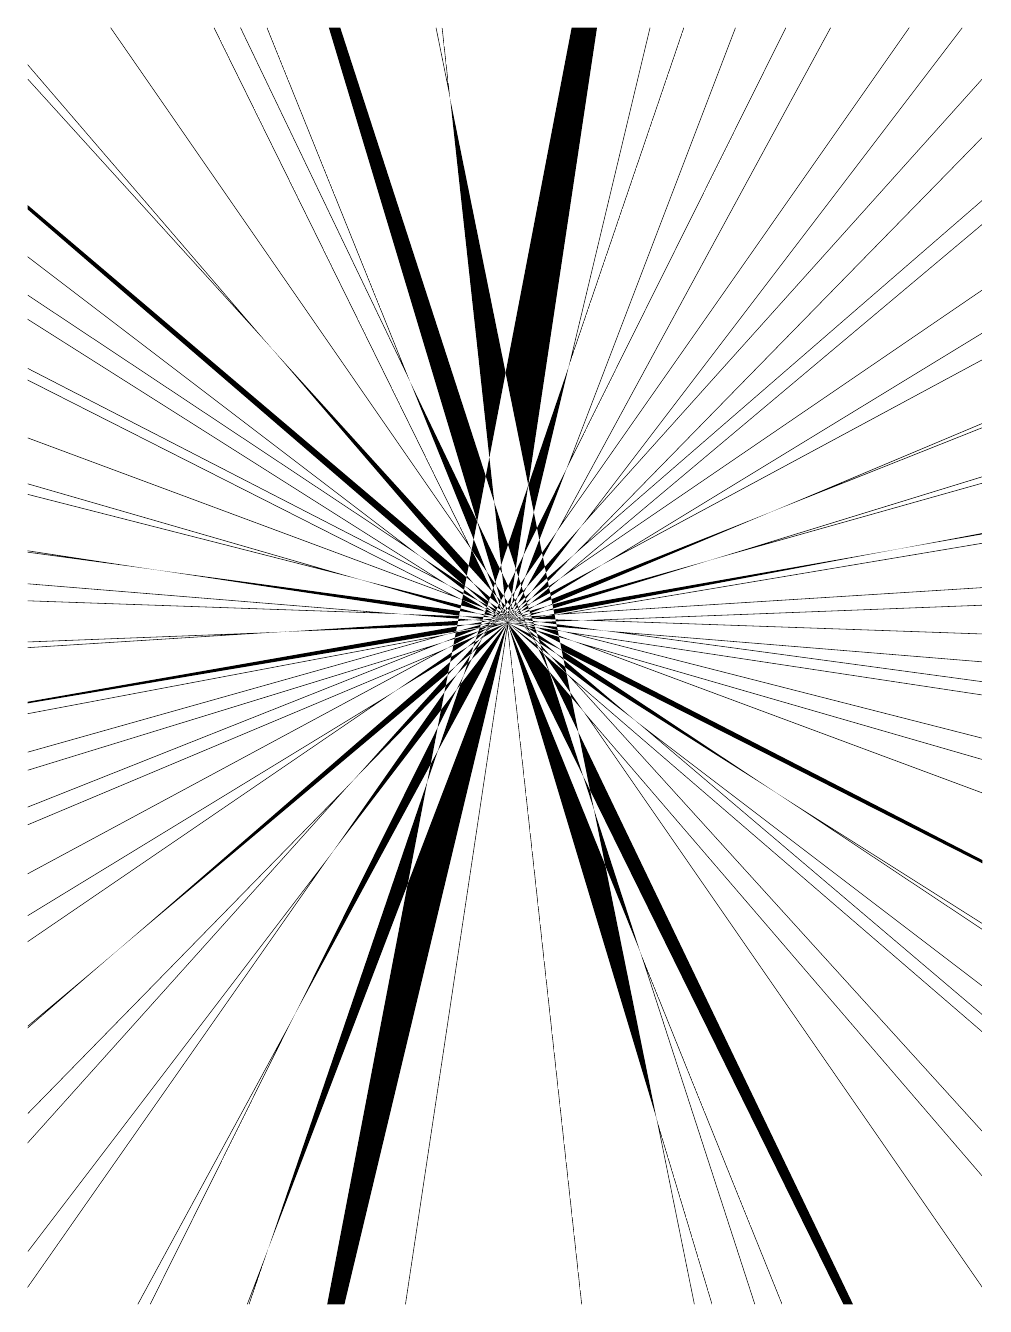
\begin{tikzpicture}[x=\linewidth,y=\linewidth]
\useasboundingbox (0,0) rectangle (1,1.33711);
\clip (0,0) rectangle (1,1.33711);
% External black cell outlines (inset)
\begin{scope}\clip (0.39539,0.00000) -- (0.58055,-0.00000) -- (0.50256,0.71333) -- cycle; \draw[line width=0.4pt] (0.58055,-0.00000) -- (0.50256,0.71333) (0.50256,0.71333) -- (0.39539,0.00000);\end{scope}
\begin{scope}\clip (0.22970,0.00000) -- (0.23216,-0.00000) -- (0.25220,0.05884) -- cycle; \draw[line width=0.4pt] (0.23216,-0.00000) -- (0.25220,0.05884) (0.25220,0.05884) -- (0.22970,0.00000);\end{scope}
\begin{scope}\clip (0.11503,0.00000) -- (0.12867,-0.00000) -- (0.28040,0.30471) -- cycle; \draw[line width=0.4pt] (0.12867,-0.00000) -- (0.28040,0.30471) (0.28040,0.30471) -- (0.11503,0.00000);\end{scope}
\begin{scope}\clip (0.00000,0.05544) -- (0.00000,0.01731) -- (0.32008,0.47467) -- cycle; \draw[line width=0.4pt] (0.00000,0.01731) -- (0.32008,0.47467) (0.32008,0.47467) -- (0.00000,0.05544);\end{scope}
\begin{scope}\clip (0.00000,0.20000) -- (0.00000,0.16863) -- (0.34177,0.54954) -- cycle; \draw[line width=0.4pt] (0.00000,0.16863) -- (0.34177,0.54954) (0.34177,0.54954) -- (0.00000,0.20000);\end{scope}
\begin{scope}\clip (0.00000,0.29159) -- (0.00000,0.28905) -- (0.09446,0.37095) -- cycle; \draw[line width=0.4pt] (0.00000,0.28905) -- (0.09446,0.37095) (0.09446,0.37095) -- (0.00000,0.29159);\end{scope}
\begin{scope}\clip (0.00000,0.37943) -- (0.38549,0.64258) -- (0.00000,0.40733) -- cycle; \draw[line width=0.4pt] (0.00000,0.37943) -- (0.38549,0.64258) (0.38549,0.64258) -- (0.00000,0.40733);\end{scope}
\begin{scope}\clip (0.00000,0.45053) -- (0.44022,0.68758) -- (0.00000,0.50248) -- cycle; \draw[line width=0.4pt] (0.00000,0.45053) -- (0.44022,0.68758) (0.44022,0.68758) -- (0.00000,0.50248);\end{scope}
\begin{scope}\clip (0.00000,0.52041) -- (0.43545,0.69349) -- (0.00000,0.55961) -- cycle; \draw[line width=0.4pt] (0.00000,0.52041) -- (0.43545,0.69349) (0.43545,0.69349) -- (0.00000,0.55961);\end{scope}
\begin{scope}\clip (0.00000,0.57795) -- (0.44018,0.70199) -- (-0.00000,0.61885) -- cycle; \draw[line width=0.4pt] (0.00000,0.57795) -- (0.44018,0.70199) (0.44018,0.70199) -- (-0.00000,0.61885);\end{scope}
\begin{scope}\clip (-0.00000,0.68744) -- (0.26857,0.70433) -- (0.00000,0.69399) -- cycle; \draw[line width=0.4pt] (-0.00000,0.68744) -- (0.26857,0.70433) (0.26857,0.70433) -- (0.00000,0.69399);\end{scope}
\begin{scope}\clip (0.71708,-0.00000) -- (0.65857,0.19479) -- (0.69799,0.00000) -- cycle; \draw[line width=0.4pt] (0.71708,-0.00000) -- (0.65857,0.19479) (0.65857,0.19479) -- (0.69799,0.00000);\end{scope}
\begin{scope}\clip (0.79047,0.00000) -- (0.64144,0.36934) -- (0.76130,0.00000) -- cycle; \draw[line width=0.4pt] (0.79047,0.00000) -- (0.64144,0.36934) (0.64144,0.36934) -- (0.76130,0.00000);\end{scope}
\begin{scope}\clip (1.00000,0.13448) -- (0.58179,0.62139) -- (1.00000,0.01706) -- cycle; \draw[line width=0.4pt] (1.00000,0.13448) -- (0.58179,0.62139) (0.58179,0.62139) -- (1.00000,0.01706);\end{scope}
\begin{scope}\clip (1.00000,0.28558) -- (0.56433,0.66078) -- (1.00000,0.18049) -- cycle; \draw[line width=0.4pt] (1.00000,0.28558) -- (0.56433,0.66078) (0.56433,0.66078) -- (1.00000,0.18049);\end{scope}
\begin{scope}\clip (1.00000,0.33358) -- (0.63601,0.61164) -- (1.00000,0.30284) -- cycle; \draw[line width=0.4pt] (1.00000,0.33358) -- (0.63601,0.61164) (0.63601,0.61164) -- (1.00000,0.30284);\end{scope}
\begin{scope}\clip (1.00000,0.39901) -- (0.78413,0.53566) -- (1.00000,0.39223) -- cycle; \draw[line width=0.4pt] (1.00000,0.39901) -- (0.78413,0.53566) (0.78413,0.53566) -- (1.00000,0.39223);\end{scope}
\begin{scope}\clip (1.00000,0.57085) -- (0.57144,0.69463) -- (1.00000,0.53524) -- cycle; \draw[line width=0.4pt] (1.00000,0.57085) -- (0.57144,0.69463) (0.57144,0.69463) -- (1.00000,0.53524);\end{scope}
\begin{scope}\clip (1.00000,0.63845) -- (0.56037,0.70487) -- (1.00000,0.59257) -- cycle; \draw[line width=0.4pt] (1.00000,0.63845) -- (0.56037,0.70487) (0.56037,0.70487) -- (1.00000,0.59257);\end{scope}
\begin{scope}\clip (1.00000,0.67315) -- (0.60335,0.70559) -- (1.00000,0.65178) -- cycle; \draw[line width=0.4pt] (1.00000,0.67315) -- (0.60335,0.70559) (0.60335,0.70559) -- (1.00000,0.65178);\end{scope}
\begin{scope}\clip (-0.00000,0.73652) -- (0.39141,0.72292) -- (0.00000,0.75493) -- cycle; \draw[line width=0.4pt] (-0.00000,0.73652) -- (0.39141,0.72292) (0.39141,0.72292) -- (0.00000,0.75493);\end{scope}
\begin{scope}\clip (0.00000,0.78744) -- (0.13545,0.76906) -- (0.00000,0.78952) -- cycle; \draw[line width=0.4pt] (0.00000,0.78744) -- (0.13545,0.76906) (0.13545,0.76906) -- (0.00000,0.78952);\end{scope}
\begin{scope}\clip (-0.00000,0.84801) -- (0.34932,0.75878) -- (0.00000,0.85967) -- cycle; \draw[line width=0.4pt] (-0.00000,0.84801) -- (0.34932,0.75878) (0.34932,0.75878) -- (0.00000,0.85967);\end{scope}
\begin{scope}\clip (-0.00000,0.90715) -- (0.45461,0.73807) -- (0.00000,0.96835) -- cycle; \draw[line width=0.4pt] (-0.00000,0.90715) -- (0.45461,0.73807) (0.45461,0.73807) -- (0.00000,0.96835);\end{scope}
\begin{scope}\clip (0.00000,0.97995) -- (0.44038,0.75326) -- (0.00000,1.03203) -- cycle; \draw[line width=0.4pt] (0.00000,0.97995) -- (0.44038,0.75326) (0.44038,0.75326) -- (0.00000,1.03203);\end{scope}
\begin{scope}\clip (-0.00000,1.05666) -- (0.41062,0.78383) -- (0.00000,1.09752) -- cycle; \draw[line width=0.4pt] (-0.00000,1.05666) -- (0.41062,0.78383) (0.41062,0.78383) -- (0.00000,1.09752);\end{scope}
\begin{scope}\clip (0.00000,1.28291) -- (0.25632,1.00033) -- (0.00000,1.29876) -- cycle; \draw[line width=0.4pt] (0.00000,1.28291) -- (0.25632,1.00033) (0.25632,1.00033) -- (0.00000,1.29876);\end{scope}
\begin{scope}\clip (0.08651,1.33711) -- (0.46498,0.79019) -- (0.19546,1.33711) -- cycle; \draw[line width=0.4pt] (0.08651,1.33711) -- (0.46498,0.79019) (0.46498,0.79019) -- (0.19546,1.33711);\end{scope}
\begin{scope}\clip (0.22255,1.33711) -- (0.40072,0.96591) -- (0.25094,1.33711) -- cycle; \draw[line width=0.4pt] (0.22255,1.33711) -- (0.40072,0.96591) (0.40072,0.96591) -- (0.25094,1.33711);\end{scope}
\begin{scope}\clip (0.42741,1.33711) -- (0.44252,1.26245) -- (0.43436,1.33711) -- cycle; \draw[line width=0.4pt] (0.42741,1.33711) -- (0.44252,1.26245) (0.44252,1.26245) -- (0.43436,1.33711);\end{scope}
\begin{scope}\clip (1.00000,0.73250) -- (0.58066,0.71635) -- (1.00000,0.70178) -- cycle; \draw[line width=0.4pt] (1.00000,0.73250) -- (0.58066,0.71635) (0.58066,0.71635) -- (1.00000,0.70178);\end{scope}
\begin{scope}\clip (1.00000,0.79741) -- (0.55210,0.72216) -- (1.00000,0.75033) -- cycle; \draw[line width=0.4pt] (1.00000,0.79741) -- (0.55210,0.72216) (0.55210,0.72216) -- (1.00000,0.75033);\end{scope}
\begin{scope}\clip (1.00000,0.80774) -- (0.91090,0.79091) -- (1.00000,0.80654) -- cycle; \draw[line width=0.4pt] (1.00000,0.80774) -- (0.91090,0.79091) (0.91090,0.79091) -- (1.00000,0.80654);\end{scope}
\begin{scope}\clip (1.00000,0.86706) -- (0.71489,0.77940) -- (1.00000,0.85975) -- cycle; \draw[line width=0.4pt] (1.00000,0.86706) -- (0.71489,0.77940) (0.71489,0.77940) -- (1.00000,0.85975);\end{scope}
\begin{scope}\clip (1.00000,0.92295) -- (0.77962,0.83029) -- (1.00000,0.91788) -- cycle; \draw[line width=0.4pt] (1.00000,0.92295) -- (0.77962,0.83029) (0.77962,0.83029) -- (1.00000,0.91788);\end{scope}
\begin{scope}\clip (1.00000,1.01761) -- (0.60165,0.77450) -- (1.00000,0.98901) -- cycle; \draw[line width=0.4pt] (1.00000,1.01761) -- (0.60165,0.77450) (0.60165,0.77450) -- (1.00000,0.98901);\end{scope}
\begin{scope}\clip (1.00000,1.13165) -- (0.55805,0.76039) -- (1.00000,1.06208) -- cycle; \draw[line width=0.4pt] (1.00000,1.13165) -- (0.55805,0.76039) (0.55805,0.76039) -- (1.00000,1.06208);\end{scope}
\begin{scope}\clip (1.00000,1.22274) -- (0.57161,0.78461) -- (1.00000,1.15600) -- cycle; \draw[line width=0.4pt] (1.00000,1.22274) -- (0.57161,0.78461) (0.57161,0.78461) -- (1.00000,1.15600);\end{scope}
\begin{scope}\clip (1.00000,1.33711) -- (0.97856,1.33711) -- (0.57978,0.81481) -- (1.00000,1.28315) -- cycle; \draw[line width=0.4pt] (0.97856,1.33711) -- (0.57978,0.81481) (0.57978,0.81481) -- (1.00000,1.28315);\end{scope}
\begin{scope}\clip (0.84069,1.33711) -- (0.55413,0.80909) -- (0.92367,1.33711) -- cycle; \draw[line width=0.4pt] (0.84069,1.33711) -- (0.55413,0.80909) (0.55413,0.80909) -- (0.92367,1.33711);\end{scope}
\begin{scope}\clip (0.74108,1.33711) -- (0.56427,0.87479) -- (0.79447,1.33711) -- cycle; \draw[line width=0.4pt] (0.74108,1.33711) -- (0.56427,0.87479) (0.56427,0.87479) -- (0.79447,1.33711);\end{scope}
\begin{scope}\clip (0.65157,1.33711) -- (0.56657,0.98177) -- (0.68761,1.33711) -- cycle; \draw[line width=0.4pt] (0.65157,1.33711) -- (0.56657,0.98177) (0.56657,0.98177) -- (0.68761,1.33711);\end{scope}
% Filled cells
\fill (0.50252,0.71334) -- (0.50256,0.71334) -- (0.50255,0.71342) -- cycle;
\fill (0.50210,0.71225) -- (0.50252,0.71334) -- (0.50236,0.71333) -- cycle;
\fill (0.50239,0.71344) -- (0.50251,0.71361) -- (0.50243,0.71362) -- cycle;
\fill (0.31374,0.00000) -- (0.33173,0.00000) -- (0.50210,0.71225) -- (0.39801,0.44008) -- cycle;
\fill (0.50230,0.71333) -- (0.50236,0.71333) -- (0.50239,0.71344) -- cycle;
\fill (0.50182,0.71270) -- (0.50230,0.71333) -- (0.50216,0.71332) -- cycle;
\fill (0.50227,0.71352) -- (0.50239,0.71363) -- (0.50233,0.71364) -- cycle;
\fill (0.42958,0.57960) -- (0.50182,0.71270) -- (0.45326,0.64909) -- cycle;
\fill (0.50202,0.71332) -- (0.50216,0.71332) -- (0.50227,0.71352) -- cycle;
\fill (0.50137,0.71277) -- (0.50202,0.71332) -- (0.50190,0.71331) -- cycle;
\fill (0.50223,0.71365) -- (0.50223,0.71365) -- (0.50223,0.71365) -- cycle;
\fill (0.46514,0.67572) -- (0.50137,0.71277) -- (0.47081,0.68710) -- cycle;
\fill (0.50139,0.71330) -- (0.50190,0.71331) -- (0.50223,0.71365) -- cycle;
\fill (0.50128,0.71325) -- (0.50139,0.71330) -- (0.50135,0.71329) -- cycle;
\fill (0.50195,0.71366) -- (0.50205,0.71368) -- (0.50200,0.71369) -- cycle;
\fill (0.47645,0.69810) -- (0.50128,0.71325) -- (0.48113,0.70478) -- cycle;
\fill (0.49966,0.71323) -- (0.50135,0.71329) -- (0.50195,0.71366) -- cycle;
\fill (0.49964,0.71322) -- (0.49966,0.71323) -- (0.49965,0.71323) -- cycle;
\fill (0.50053,0.71350) -- (0.50181,0.71371) -- (0.50142,0.71377) -- cycle;
\fill (0.48444,0.70855) -- (0.49964,0.71322) -- (0.48639,0.71072) -- cycle;
\fill (0.49870,0.71319) -- (0.49965,0.71323) -- (0.50053,0.71350) -- cycle;
\fill (0.48696,0.71122) -- (0.49870,0.71319) -- (0.48879,0.71281) -- cycle;
\fill (0.49040,0.71421) -- (0.49121,0.71476) -- (0.49106,0.71477) -- cycle;
\fill (0.48641,0.71074) -- (0.48696,0.71122) -- (0.48681,0.71119) -- cycle;
\fill (0.48833,0.71279) -- (0.48879,0.71281) -- (0.49040,0.71421) -- cycle;
\fill (0.48811,0.71264) -- (0.48833,0.71279) -- (0.48824,0.71279) -- cycle;
\fill (0.48937,0.71404) -- (0.49077,0.71480) -- (0.49009,0.71485) -- cycle;
\fill (0.48138,0.70514) -- (0.48444,0.70855) -- (0.48358,0.70829) -- cycle;
\fill (0.48638,0.71072) -- (0.48639,0.71072) -- (0.48641,0.71074) -- cycle;
\fill (0.48359,0.70830) -- (0.48638,0.71072) -- (0.48512,0.71048) -- cycle;
\fill (0.48572,0.71101) -- (0.48681,0.71119) -- (0.48811,0.71264) -- cycle;
\fill (0.48528,0.71071) -- (0.48572,0.71101) -- (0.48546,0.71097) -- cycle;
\fill (0.48695,0.71274) -- (0.48824,0.71279) -- (0.48937,0.71404) -- cycle;
\fill (0.48655,0.71252) -- (0.48695,0.71274) -- (0.48669,0.71273) -- cycle;
\fill (0.48778,0.71429) -- (0.48935,0.71491) -- (0.48828,0.71500) -- cycle;
\fill (0.47587,0.69727) -- (0.47645,0.69810) -- (0.47621,0.69795) -- cycle;
\fill (0.48101,0.70473) -- (0.48113,0.70478) -- (0.48138,0.70514) -- cycle;
\fill (0.47781,0.70116) -- (0.48101,0.70473) -- (0.47921,0.70397) -- cycle;
\fill (0.48357,0.70829) -- (0.48358,0.70829) -- (0.48359,0.70830) -- cycle;
\fill (0.47967,0.70490) -- (0.48357,0.70829) -- (0.48096,0.70748) -- cycle;
\fill (0.48488,0.71044) -- (0.48512,0.71048) -- (0.48528,0.71071) -- cycle;
\fill (0.48116,0.70790) -- (0.48488,0.71044) -- (0.48217,0.70993) -- cycle;
\fill (0.48284,0.71053) -- (0.48546,0.71097) -- (0.48655,0.71252) -- cycle;
\fill (0.48234,0.71026) -- (0.48284,0.71053) -- (0.48244,0.71046) -- cycle;
\fill (0.48355,0.71261) -- (0.48669,0.71273) -- (0.48778,0.71429) -- cycle;
\fill (0.48350,0.71259) -- (0.48355,0.71261) -- (0.48351,0.71261) -- cycle;
\fill (0.48443,0.71446) -- (0.48677,0.71512) -- (0.48484,0.71528) -- cycle;
\fill (0.45623,0.65782) -- (0.46514,0.67572) -- (0.46082,0.67130) -- cycle;
\fill (0.46582,0.68291) -- (0.47081,0.68710) -- (0.47587,0.69727) -- cycle;
\fill (0.46378,0.67999) -- (0.46582,0.68291) -- (0.46435,0.68168) -- cycle;
\fill (0.47338,0.69622) -- (0.47621,0.69795) -- (0.47781,0.70116) -- cycle;
\fill (0.46682,0.68891) -- (0.47338,0.69622) -- (0.46824,0.69309) -- cycle;
\fill (0.47802,0.70347) -- (0.47921,0.70397) -- (0.47967,0.70490) -- cycle;
\fill (0.46916,0.69579) -- (0.47802,0.70347) -- (0.47073,0.70041) -- cycle;
\fill (0.48022,0.70725) -- (0.48096,0.70748) -- (0.48116,0.70790) -- cycle;
\fill (0.47090,0.70089) -- (0.48022,0.70725) -- (0.47223,0.70480) -- cycle;
\fill (0.48148,0.70979) -- (0.48217,0.70993) -- (0.48234,0.71026) -- cycle;
\fill (0.47224,0.70482) -- (0.48148,0.70979) -- (0.47341,0.70827) -- cycle;
\fill (0.47500,0.70921) -- (0.48244,0.71046) -- (0.48350,0.71259) -- cycle;
\fill (0.47353,0.70863) -- (0.47500,0.70921) -- (0.47366,0.70898) -- cycle;
\fill (0.47695,0.71235) -- (0.48351,0.71261) -- (0.48443,0.71446) -- cycle;
\fill (0.47458,0.71169) -- (0.47695,0.71235) -- (0.47478,0.71227) -- cycle;
\fill (0.47553,0.71449) -- (0.48157,0.71555) -- (0.47605,0.71600) -- cycle;
\fill (0.41849,0.54702) -- (0.42958,0.57960) -- (0.42208,0.56576) -- cycle;
\fill (0.44931,0.64392) -- (0.45326,0.64909) -- (0.45623,0.65782) -- cycle;
\fill (0.42938,0.60390) -- (0.44931,0.64392) -- (0.43294,0.62248) -- cycle;
\fill (0.44983,0.66006) -- (0.46082,0.67130) -- (0.46378,0.67999) -- cycle;
\fill (0.43648,0.64098) -- (0.44983,0.66006) -- (0.43777,0.64773) -- cycle;
\fill (0.44800,0.66794) -- (0.46435,0.68168) -- (0.46682,0.68891) -- cycle;
\fill (0.43992,0.65893) -- (0.44800,0.66794) -- (0.44042,0.66157) -- cycle;
\fill (0.46082,0.68856) -- (0.46824,0.69309) -- (0.46916,0.69579) -- cycle;
\fill (0.44256,0.67273) -- (0.46082,0.68856) -- (0.44358,0.67803) -- cycle;
\fill (0.46931,0.69981) -- (0.47073,0.70041) -- (0.47090,0.70089) -- cycle;
\fill (0.44450,0.68287) -- (0.46931,0.69981) -- (0.44586,0.68995) -- cycle;
\fill (0.47216,0.70478) -- (0.47223,0.70480) -- (0.47224,0.70482) -- cycle;
\fill (0.44600,0.69069) -- (0.47216,0.70478) -- (0.44723,0.69711) -- cycle;
\fill (0.47194,0.70799) -- (0.47341,0.70827) -- (0.47353,0.70863) -- cycle;
\fill (0.44745,0.69826) -- (0.47194,0.70799) -- (0.44846,0.70356) -- cycle;
\fill (0.45219,0.70538) -- (0.47366,0.70898) -- (0.47458,0.71169) -- cycle;
\fill (0.44862,0.70437) -- (0.45219,0.70538) -- (0.44870,0.70479) -- cycle;
\fill (0.45955,0.71168) -- (0.47478,0.71227) -- (0.47553,0.71449) -- cycle;
\fill (0.44969,0.70995) -- (0.45955,0.71168) -- (0.44995,0.71131) -- cycle;
\fill (0.45081,0.71579) -- (0.46651,0.71678) -- (0.45123,0.71803) -- cycle;
\fill (0.25220,0.05884) -- (0.39801,0.44008) -- (0.41849,0.54702) -- cycle;
\fill (0.28040,0.30471) -- (0.42208,0.56576) -- (0.42938,0.60390) -- cycle;
\fill (0.32008,0.47467) -- (0.43294,0.62248) -- (0.43648,0.64098) -- cycle;
\fill (0.34177,0.54954) -- (0.43777,0.64773) -- (0.43992,0.65893) -- cycle;
\fill (0.09446,0.37095) -- (0.44042,0.66157) -- (0.44256,0.67273) -- cycle;
\fill (0.38549,0.64258) -- (0.44358,0.67803) -- (0.44450,0.68287) -- cycle;
\fill (0.44022,0.68758) -- (0.44586,0.68995) -- (0.44600,0.69069) -- cycle;
\fill (0.43545,0.69349) -- (0.44723,0.69711) -- (0.44745,0.69826) -- cycle;
\fill (0.44018,0.70199) -- (0.44846,0.70356) -- (0.44862,0.70437) -- cycle;
\fill (-0.00000,0.63102) -- (0.00000,0.62941) -- (0.44870,0.70479) -- (0.44969,0.70995) -- cycle;
\fill (0.26857,0.70433) -- (0.44995,0.71131) -- (0.45081,0.71579) -- cycle;
\fill (0.50256,0.71334) -- (0.50263,0.71334) -- (0.50258,0.71348) -- cycle;
\fill (0.50256,0.71334) -- (0.50256,0.71333) -- (0.50256,0.71334) -- cycle;
\fill (0.50253,0.71360) -- (0.50255,0.71342) -- (0.50257,0.71349) -- cycle;
\fill (0.50332,0.71163) -- (0.65857,0.19479) -- (0.60495,0.45977) -- cycle;
\fill (0.50253,0.71361) -- (0.50253,0.71360) -- (0.50253,0.71361) -- cycle;
\fill (0.50263,0.71334) -- (0.50332,0.71163) -- (0.50281,0.71335) -- cycle;
\fill (0.50259,0.71351) -- (0.50260,0.71356) -- (0.50259,0.71357) -- cycle;
\fill (0.50257,0.71349) -- (0.50258,0.71348) -- (0.50259,0.71351) -- cycle;
\fill (0.50281,0.71336) -- (0.50281,0.71335) -- (0.50281,0.71335) -- cycle;
\fill (0.59312,0.51822) -- (0.60495,0.45977) -- (0.64144,0.36934) -- cycle;
\fill (0.58177,0.55321) -- (0.59312,0.51822) -- (0.58902,0.53849) -- cycle;
\fill (0.50290,0.71324) -- (0.58177,0.55321) -- (0.54618,0.66285) -- cycle;
\fill (0.86436,0.00000) -- (0.57673,0.59923) -- (0.58902,0.53849) -- (0.85439,0.00000) -- cycle;
\fill (0.54620,0.66284) -- (0.57673,0.59923) -- (0.56930,0.63594) -- cycle;
\fill (0.50268,0.71350) -- (0.50281,0.71336) -- (0.50279,0.71342) -- cycle;
\fill (0.50281,0.71335) -- (0.50290,0.71324) -- (0.50285,0.71335) -- cycle;
\fill (0.50283,0.71339) -- (0.50285,0.71335) -- (0.50288,0.71335) -- cycle;
\fill (0.54617,0.66289) -- (0.54618,0.66285) -- (0.54620,0.66284) -- cycle;
\fill (0.53510,0.68595) -- (0.54617,0.66289) -- (0.54008,0.68166) -- cycle;
\fill (0.56830,0.64089) -- (0.56930,0.63594) -- (0.58179,0.62139) -- cycle;
\fill (0.54009,0.68165) -- (0.56830,0.64089) -- (0.56426,0.66083) -- cycle;
\fill (0.50646,0.71061) -- (0.53510,0.68595) -- (0.53299,0.69035) -- cycle;
\fill (0.54007,0.68168) -- (0.54008,0.68166) -- (0.54009,0.68165) -- cycle;
\fill (0.53529,0.68859) -- (0.54007,0.68168) -- (0.53867,0.68601) -- cycle;
\fill (0.56426,0.66086) -- (0.56426,0.66083) -- (0.56433,0.66078) -- cycle;
\fill (0.54770,0.67911) -- (0.56426,0.66086) -- (0.56292,0.66748) -- cycle;
\fill (0.50260,0.71356) -- (0.50268,0.71350) -- (0.50261,0.71358) -- cycle;
\fill (0.50255,0.71360) -- (0.50259,0.71357) -- (0.50260,0.71360) -- cycle;
\fill (0.50260,0.71360) -- (0.50261,0.71358) -- (0.50262,0.71359) -- cycle;
\fill (0.50274,0.71357) -- (0.50279,0.71342) -- (0.50283,0.71339) -- cycle;
\fill (0.50274,0.71358) -- (0.50274,0.71357) -- (0.50274,0.71358) -- cycle;
\fill (0.50288,0.71335) -- (0.50646,0.71061) -- (0.50326,0.71337) -- cycle;
\fill (0.50308,0.71352) -- (0.50326,0.71337) -- (0.50338,0.71337) -- cycle;
\fill (0.53054,0.69546) -- (0.53299,0.69035) -- (0.53529,0.68859) -- cycle;
\fill (0.52964,0.69676) -- (0.53054,0.69546) -- (0.53004,0.69651) -- cycle;
\fill (0.53712,0.69077) -- (0.53867,0.68601) -- (0.54770,0.67911) -- cycle;
\fill (0.53446,0.69370) -- (0.53712,0.69077) -- (0.53661,0.69234) -- cycle;
\fill (0.56141,0.67494) -- (0.56292,0.66748) -- (0.63601,0.61164) -- cycle;
\fill (0.55347,0.68167) -- (0.56141,0.67494) -- (0.56101,0.67690) -- cycle;
\fill (0.50344,0.71334) -- (0.52964,0.69676) -- (0.52611,0.70186) -- cycle;
\fill (0.52792,0.70092) -- (0.53004,0.69651) -- (0.53446,0.69370) -- cycle;
\fill (0.52788,0.70096) -- (0.52792,0.70092) -- (0.52790,0.70095) -- cycle;
\fill (0.53499,0.69735) -- (0.53661,0.69234) -- (0.55347,0.68167) -- cycle;
\fill (0.53496,0.69737) -- (0.53499,0.69735) -- (0.53498,0.69736) -- cycle;
\fill (0.55937,0.68500) -- (0.56101,0.67690) -- (0.78413,0.53566) -- cycle;
\fill (0.55929,0.68505) -- (0.55937,0.68500) -- (0.55937,0.68501) -- cycle;
\fill (0.50308,0.71352) -- (0.50308,0.71352) -- (0.50308,0.71352) -- cycle;
\fill (0.50338,0.71337) -- (0.50344,0.71334) -- (0.50339,0.71337) -- cycle;
\fill (0.50318,0.71351) -- (0.50339,0.71337) -- (0.50394,0.71339) -- cycle;
\fill (0.52303,0.70631) -- (0.52611,0.70186) -- (0.52788,0.70096) -- cycle;
\fill (0.52020,0.70943) -- (0.52303,0.70631) -- (0.52104,0.70918) -- cycle;
\fill (0.52595,0.70502) -- (0.52790,0.70095) -- (0.53496,0.69737) -- cycle;
\fill (0.52105,0.70918) -- (0.52595,0.70502) -- (0.52442,0.70821) -- cycle;
\fill (0.53340,0.70226) -- (0.53498,0.69736) -- (0.55929,0.68505) -- cycle;
\fill (0.52445,0.70820) -- (0.53340,0.70226) -- (0.53219,0.70596) -- cycle;
\fill (1.00000,0.46519) -- (0.55779,0.69282) -- (0.55937,0.68501) -- (1.00000,0.46182) -- cycle;
\fill (0.53235,0.70592) -- (0.55779,0.69282) -- (0.55655,0.69893) -- cycle;
\fill (0.50923,0.71259) -- (0.52020,0.70943) -- (0.51861,0.71118) -- cycle;
\fill (0.52104,0.70919) -- (0.52104,0.70918) -- (0.52105,0.70918) -- cycle;
\fill (0.51871,0.71116) -- (0.52104,0.70919) -- (0.51978,0.71100) -- cycle;
\fill (0.52441,0.70823) -- (0.52442,0.70821) -- (0.52445,0.70820) -- cycle;
\fill (0.52037,0.71091) -- (0.52441,0.70823) -- (0.52334,0.71046) -- cycle;
\fill (0.53218,0.70600) -- (0.53219,0.70596) -- (0.53235,0.70592) -- cycle;
\fill (0.52359,0.71043) -- (0.53218,0.70600) -- (0.53111,0.70929) -- cycle;
\fill (0.55628,0.70026) -- (0.55655,0.69893) -- (0.57144,0.69463) -- cycle;
\fill (0.53263,0.70906) -- (0.55628,0.70026) -- (0.55519,0.70565) -- cycle;
\fill (0.50251,0.71361) -- (0.50253,0.71361) -- (0.50252,0.71362) -- cycle;
\fill (0.50244,0.71367) -- (0.50245,0.71368) -- (0.50244,0.71368) -- cycle;
\fill (0.50239,0.71363) -- (0.50243,0.71362) -- (0.50244,0.71367) -- cycle;
\fill (0.50237,0.71371) -- (0.50240,0.71372) -- (0.50238,0.71373) -- cycle;
\fill (0.50223,0.71365) -- (0.50233,0.71364) -- (0.50237,0.71371) -- cycle;
\fill (0.50231,0.71373) -- (0.50237,0.71374) -- (0.50234,0.71376) -- cycle;
\fill (0.50205,0.71368) -- (0.50223,0.71365) -- (0.50231,0.71373) -- cycle;
\fill (0.50213,0.71377) -- (0.50230,0.71380) -- (0.50224,0.71384) -- cycle;
\fill (0.50181,0.71371) -- (0.50200,0.71369) -- (0.50213,0.71377) -- cycle;
\fill (0.49925,0.71410) -- (0.50142,0.71377) -- (0.50181,0.71389) -- cycle;
\fill (0.50252,0.71363) -- (0.50252,0.71362) -- (0.50252,0.71362) -- cycle;
\fill (0.50253,0.71362) -- (0.50253,0.71361) -- (0.50255,0.71360) -- cycle;
\fill (0.50245,0.71368) -- (0.50252,0.71363) -- (0.50249,0.71371) -- cycle;
\fill (0.50246,0.71375) -- (0.50247,0.71375) -- (0.50246,0.71376) -- cycle;
\fill (0.50240,0.71372) -- (0.50244,0.71368) -- (0.50246,0.71375) -- cycle;
\fill (0.50239,0.71374) -- (0.50246,0.71376) -- (0.50242,0.71381) -- cycle;
\fill (0.50237,0.71374) -- (0.50238,0.71373) -- (0.50239,0.71374) -- cycle;
\fill (0.50239,0.71381) -- (0.50241,0.71382) -- (0.50240,0.71383) -- cycle;
\fill (0.50230,0.71380) -- (0.50234,0.71376) -- (0.50239,0.71381) -- cycle;
\fill (0.50221,0.71386) -- (0.50224,0.71384) -- (0.50227,0.71386) -- cycle;
\fill (0.50252,0.71362) -- (0.50253,0.71362) -- (0.50253,0.71362) -- cycle;
\fill (0.50247,0.71375) -- (0.50249,0.71371) -- (0.50250,0.71372) -- cycle;
\fill (0.50260,0.71360) -- (0.50260,0.71360) -- (0.50260,0.71360) -- cycle;
\fill (0.50252,0.71369) -- (0.50253,0.71362) -- (0.50255,0.71365) -- cycle;
\fill (0.50247,0.71375) -- (0.50247,0.71375) -- (0.50247,0.71375) -- cycle;
\fill (0.50246,0.71376) -- (0.50247,0.71376) -- (0.50246,0.71376) -- cycle;
\fill (0.50246,0.71376) -- (0.50246,0.71376) -- (0.50246,0.71376) -- cycle;
\fill (0.50243,0.71382) -- (0.50244,0.71382) -- (0.50243,0.71383) -- cycle;
\fill (0.50241,0.71382) -- (0.50242,0.71381) -- (0.50243,0.71382) -- cycle;
\fill (0.50239,0.71385) -- (0.50240,0.71383) -- (0.50242,0.71384) -- cycle;
\fill (0.50250,0.71372) -- (0.50252,0.71369) -- (0.50251,0.71373) -- cycle;
\fill (0.50251,0.71377) -- (0.50251,0.71377) -- (0.50251,0.71377) -- cycle;
\fill (0.50247,0.71376) -- (0.50247,0.71375) -- (0.50251,0.71377) -- cycle;
\fill (0.50248,0.71383) -- (0.50248,0.71383) -- (0.50248,0.71383) -- cycle;
\fill (0.50244,0.71382) -- (0.50246,0.71376) -- (0.50248,0.71383) -- cycle;
\fill (0.50243,0.71384) -- (0.50243,0.71383) -- (0.50244,0.71384) -- cycle;
\fill (0.50262,0.71359) -- (0.50274,0.71358) -- (0.50267,0.71372) -- cycle;
\fill (0.50262,0.71375) -- (0.50263,0.71375) -- (0.50262,0.71376) -- cycle;
\fill (0.50255,0.71365) -- (0.50260,0.71360) -- (0.50262,0.71375) -- cycle;
\fill (0.50257,0.71378) -- (0.50258,0.71378) -- (0.50257,0.71378) -- cycle;
\fill (0.50251,0.71377) -- (0.50251,0.71373) -- (0.50257,0.71378) -- cycle;
\fill (0.50251,0.71382) -- (0.50251,0.71377) -- (0.50256,0.71379) -- cycle;
\fill (0.50266,0.71374) -- (0.50267,0.71372) -- (0.50267,0.71373) -- cycle;
\fill (0.50270,0.71372) -- (0.50274,0.71358) -- (0.50308,0.71352) -- cycle;
\fill (0.50248,0.71383) -- (0.50251,0.71382) -- (0.50250,0.71383) -- cycle;
\fill (0.50246,0.71384) -- (0.50248,0.71383) -- (0.50248,0.71384) -- cycle;
\fill (0.50263,0.71375) -- (0.50266,0.71374) -- (0.50264,0.71377) -- cycle;
\fill (0.50263,0.71379) -- (0.50263,0.71379) -- (0.50263,0.71380) -- cycle;
\fill (0.50258,0.71378) -- (0.50262,0.71376) -- (0.50263,0.71379) -- cycle;
\fill (0.50260,0.71381) -- (0.50262,0.71381) -- (0.50262,0.71382) -- cycle;
\fill (0.50256,0.71379) -- (0.50257,0.71378) -- (0.50260,0.71381) -- cycle;
\fill (0.50250,0.71384) -- (0.50250,0.71383) -- (0.50253,0.71383) -- cycle;
\fill (0.50267,0.71373) -- (0.50270,0.71372) -- (0.50268,0.71377) -- cycle;
\fill (0.50266,0.71379) -- (0.50267,0.71380) -- (0.50267,0.71381) -- cycle;
\fill (0.50263,0.71379) -- (0.50264,0.71377) -- (0.50266,0.71379) -- cycle;
\fill (0.50263,0.71382) -- (0.50264,0.71382) -- (0.50263,0.71383) -- cycle;
\fill (0.50262,0.71381) -- (0.50263,0.71380) -- (0.50263,0.71382) -- cycle;
\fill (0.50261,0.71383) -- (0.50262,0.71382) -- (0.50263,0.71383) -- cycle;
\fill (0.50270,0.71380) -- (0.50271,0.71380) -- (0.50270,0.71381) -- cycle;
\fill (0.50267,0.71380) -- (0.50268,0.71377) -- (0.50270,0.71380) -- cycle;
\fill (0.50267,0.71382) -- (0.50267,0.71381) -- (0.50268,0.71382) -- cycle;
\fill (0.50289,0.71369) -- (0.50308,0.71352) -- (0.50318,0.71351) -- cycle;
\fill (0.50271,0.71380) -- (0.50289,0.71369) -- (0.50275,0.71381) -- cycle;
\fill (0.50268,0.71382) -- (0.50270,0.71381) -- (0.50270,0.71382) -- cycle;
\fill (0.50394,0.71339) -- (0.50923,0.71259) -- (0.50617,0.71348) -- cycle;
\fill (0.50274,0.71382) -- (0.50275,0.71381) -- (0.50276,0.71381) -- cycle;
\fill (0.50589,0.71356) -- (0.50617,0.71348) -- (0.50664,0.71350) -- cycle;
\fill (0.51834,0.71148) -- (0.51861,0.71118) -- (0.51871,0.71116) -- cycle;
\fill (0.51695,0.71265) -- (0.51834,0.71148) -- (0.51730,0.71263) -- cycle;
\fill (0.51940,0.71156) -- (0.51978,0.71100) -- (0.52037,0.71091) -- cycle;
\fill (0.51786,0.71258) -- (0.51940,0.71156) -- (0.51874,0.71251) -- cycle;
\fill (0.52328,0.71059) -- (0.52334,0.71046) -- (0.52359,0.71043) -- cycle;
\fill (0.51970,0.71243) -- (0.52328,0.71059) -- (0.52250,0.71220) -- cycle;
\fill (0.53099,0.70967) -- (0.53111,0.70929) -- (0.53263,0.70906) -- cycle;
\fill (0.52466,0.71202) -- (0.53099,0.70967) -- (0.53038,0.71156) -- cycle;
\fill (0.55508,0.70622) -- (0.55519,0.70565) -- (0.56037,0.70487) -- cycle;
\fill (0.53599,0.71110) -- (0.55508,0.70622) -- (0.55440,0.70959) -- cycle;
\fill (0.49121,0.71476) -- (0.49925,0.71410) -- (0.49188,0.71522) -- cycle;
\fill (0.49160,0.71524) -- (0.49162,0.71525) -- (0.49161,0.71526) -- cycle;
\fill (0.49077,0.71480) -- (0.49106,0.71477) -- (0.49160,0.71524) -- cycle;
\fill (0.49059,0.71541) -- (0.49060,0.71541) -- (0.49059,0.71541) -- cycle;
\fill (0.48935,0.71491) -- (0.49009,0.71485) -- (0.49059,0.71541) -- cycle;
\fill (0.48876,0.71568) -- (0.48877,0.71569) -- (0.48876,0.71569) -- cycle;
\fill (0.48677,0.71512) -- (0.48828,0.71500) -- (0.48876,0.71568) -- cycle;
\fill (0.48530,0.71620) -- (0.48532,0.71621) -- (0.48530,0.71621) -- cycle;
\fill (0.48157,0.71555) -- (0.48484,0.71528) -- (0.48530,0.71620) -- cycle;
\fill (0.47653,0.71741) -- (0.47711,0.71745) -- (0.47657,0.71753) -- cycle;
\fill (0.46651,0.71678) -- (0.47605,0.71600) -- (0.47653,0.71741) -- cycle;
\fill (0.39141,0.72292) -- (0.45123,0.71803) -- (0.45177,0.72082) -- cycle;
\fill (0.50181,0.71389) -- (0.50221,0.71386) -- (0.50207,0.71397) -- cycle;
\fill (0.49313,0.71607) -- (0.49455,0.71683) -- (0.49434,0.71689) -- cycle;
\fill (0.49162,0.71525) -- (0.49188,0.71522) -- (0.49313,0.71607) -- cycle;
\fill (0.49280,0.71628) -- (0.49434,0.71690) -- (0.49371,0.71708) -- cycle;
\fill (0.49060,0.71541) -- (0.49161,0.71526) -- (0.49280,0.71628) -- cycle;
\fill (0.49154,0.71647) -- (0.49371,0.71708) -- (0.49242,0.71745) -- cycle;
\fill (0.48877,0.71569) -- (0.49059,0.71541) -- (0.49154,0.71647) -- cycle;
\fill (0.48966,0.71697) -- (0.49241,0.71745) -- (0.49040,0.71803) -- cycle;
\fill (0.48532,0.71621) -- (0.48876,0.71569) -- (0.48966,0.71697) -- cycle;
\fill (0.48620,0.71802) -- (0.48969,0.71824) -- (0.48674,0.71909) -- cycle;
\fill (0.47711,0.71745) -- (0.48530,0.71621) -- (0.48620,0.71802) -- cycle;
\fill (0.45564,0.72069) -- (0.47657,0.71753) -- (0.47739,0.71993) -- cycle;
\fill (0.50227,0.71386) -- (0.50239,0.71385) -- (0.50234,0.71390) -- cycle;
\fill (0.50181,0.71417) -- (0.50207,0.71397) -- (0.50215,0.71400) -- cycle;
\fill (0.50242,0.71384) -- (0.50243,0.71384) -- (0.50243,0.71385) -- cycle;
\fill (0.50234,0.71390) -- (0.50234,0.71390) -- (0.50234,0.71390) -- cycle;
\fill (0.50244,0.71384) -- (0.50246,0.71384) -- (0.50244,0.71385) -- cycle;
\fill (0.50243,0.71386) -- (0.50243,0.71385) -- (0.50243,0.71385) -- cycle;
\fill (0.49919,0.71549) -- (0.50181,0.71417) -- (0.50061,0.71508) -- cycle;
\fill (0.50215,0.71400) -- (0.50234,0.71390) -- (0.50223,0.71402) -- cycle;
\fill (0.50234,0.71390) -- (0.50243,0.71386) -- (0.50240,0.71393) -- cycle;
\fill (0.50208,0.71420) -- (0.50223,0.71402) -- (0.50232,0.71405) -- cycle;
\fill (0.50248,0.71384) -- (0.50250,0.71384) -- (0.50250,0.71390) -- cycle;
\fill (0.50247,0.71389) -- (0.50249,0.71392) -- (0.50249,0.71394) -- cycle;
\fill (0.50243,0.71385) -- (0.50244,0.71385) -- (0.50247,0.71389) -- cycle;
\fill (0.50236,0.71403) -- (0.50240,0.71393) -- (0.50245,0.71397) -- cycle;
\fill (0.50253,0.71383) -- (0.50261,0.71383) -- (0.50260,0.71385) -- cycle;
\fill (0.50250,0.71393) -- (0.50251,0.71393) -- (0.50250,0.71393) -- cycle;
\fill (0.50249,0.71392) -- (0.50250,0.71390) -- (0.50250,0.71393) -- cycle;
\fill (0.50249,0.71394) -- (0.50249,0.71394) -- (0.50249,0.71394) -- cycle;
\fill (0.50264,0.71382) -- (0.50267,0.71382) -- (0.50266,0.71383) -- cycle;
\fill (0.50263,0.71383) -- (0.50265,0.71384) -- (0.50264,0.71385) -- cycle;
\fill (0.50263,0.71383) -- (0.50263,0.71383) -- (0.50263,0.71383) -- cycle;
\fill (0.50259,0.71388) -- (0.50260,0.71385) -- (0.50263,0.71385) -- cycle;
\fill (0.50268,0.71382) -- (0.50268,0.71382) -- (0.50268,0.71382) -- cycle;
\fill (0.50266,0.71383) -- (0.50266,0.71383) -- (0.50266,0.71383) -- cycle;
\fill (0.50075,0.71504) -- (0.50208,0.71420) -- (0.50156,0.71481) -- cycle;
\fill (0.50232,0.71405) -- (0.50236,0.71403) -- (0.50234,0.71406) -- cycle;
\fill (0.50245,0.71397) -- (0.50249,0.71394) -- (0.50249,0.71399) -- cycle;
\fill (0.50228,0.71421) -- (0.50234,0.71406) -- (0.50243,0.71408) -- cycle;
\fill (0.50251,0.71393) -- (0.50259,0.71388) -- (0.50254,0.71397) -- cycle;
\fill (0.50252,0.71399) -- (0.50253,0.71400) -- (0.50252,0.71401) -- cycle;
\fill (0.50249,0.71394) -- (0.50250,0.71393) -- (0.50252,0.71399) -- cycle;
\fill (0.50248,0.71404) -- (0.50249,0.71399) -- (0.50252,0.71401) -- cycle;
\fill (0.50265,0.71384) -- (0.50266,0.71383) -- (0.50266,0.71385) -- cycle;
\fill (0.50264,0.71385) -- (0.50266,0.71386) -- (0.50264,0.71390) -- cycle;
\fill (0.50263,0.71385) -- (0.50264,0.71385) -- (0.50264,0.71385) -- cycle;
\fill (0.50253,0.71400) -- (0.50254,0.71397) -- (0.50255,0.71398) -- cycle;
\fill (0.50270,0.71382) -- (0.50274,0.71382) -- (0.50271,0.71384) -- cycle;
\fill (0.50269,0.71385) -- (0.50270,0.71385) -- (0.50270,0.71385) -- cycle;
\fill (0.50266,0.71383) -- (0.50268,0.71382) -- (0.50269,0.71385) -- cycle;
\fill (0.50266,0.71386) -- (0.50269,0.71386) -- (0.50268,0.71387) -- cycle;
\fill (0.50266,0.71386) -- (0.50266,0.71385) -- (0.50266,0.71386) -- cycle;
\fill (0.50264,0.71390) -- (0.50264,0.71390) -- (0.50264,0.71390) -- cycle;
\fill (0.50160,0.71480) -- (0.50228,0.71421) -- (0.50210,0.71465) -- cycle;
\fill (0.50243,0.71408) -- (0.50248,0.71404) -- (0.50247,0.71410) -- cycle;
\fill (0.50253,0.71400) -- (0.50253,0.71400) -- (0.50253,0.71400) -- cycle;
\fill (0.50252,0.71401) -- (0.50252,0.71401) -- (0.50252,0.71401) -- cycle;
\fill (0.50252,0.71401) -- (0.50252,0.71401) -- (0.50252,0.71401) -- cycle;
\fill (0.50247,0.71412) -- (0.50247,0.71410) -- (0.50248,0.71410) -- cycle;
\fill (0.50223,0.71462) -- (0.50247,0.71412) -- (0.50242,0.71456) -- cycle;
\fill (0.50255,0.71398) -- (0.50264,0.71390) -- (0.50260,0.71403) -- cycle;
\fill (0.50253,0.71402) -- (0.50260,0.71405) -- (0.50258,0.71410) -- cycle;
\fill (0.50252,0.71401) -- (0.50253,0.71400) -- (0.50253,0.71402) -- cycle;
\fill (0.50255,0.71412) -- (0.50257,0.71413) -- (0.50256,0.71417) -- cycle;
\fill (0.50248,0.71410) -- (0.50252,0.71401) -- (0.50255,0.71412) -- cycle;
\fill (0.50276,0.71381) -- (0.50589,0.71356) -- (0.50412,0.71407) -- cycle;
\fill (0.50276,0.71387) -- (0.50405,0.71409) -- (0.50359,0.71422) -- cycle;
\fill (0.50272,0.71385) -- (0.50276,0.71387) -- (0.50272,0.71387) -- cycle;
\fill (0.50322,0.71433) -- (0.50323,0.71433) -- (0.50322,0.71433) -- cycle;
\fill (0.50278,0.71395) -- (0.50322,0.71433) -- (0.50301,0.71426) -- cycle;
\fill (0.50308,0.71435) -- (0.50310,0.71436) -- (0.50309,0.71437) -- cycle;
\fill (0.50273,0.71389) -- (0.50278,0.71395) -- (0.50274,0.71392) -- cycle;
\fill (0.50286,0.71422) -- (0.50301,0.71426) -- (0.50308,0.71435) -- cycle;
\fill (0.50285,0.71421) -- (0.50286,0.71422) -- (0.50285,0.71421) -- cycle;
\fill (0.50290,0.71433) -- (0.50297,0.71440) -- (0.50293,0.71441) -- cycle;
\fill (0.50270,0.71385) -- (0.50271,0.71384) -- (0.50272,0.71385) -- cycle;
\fill (0.50271,0.71387) -- (0.50272,0.71387) -- (0.50273,0.71389) -- cycle;
\fill (0.50269,0.71386) -- (0.50270,0.71385) -- (0.50271,0.71387) -- cycle;
\fill[red] (0.50264,0.71390) -- (0.50268,0.71387) -- (0.50274,0.71392) -- (0.50285,0.71421) -- (0.50267,0.71410) -- cycle;
\fill (0.50275,0.71418) -- (0.50285,0.71421) -- (0.50290,0.71433) -- cycle;
\fill (0.50267,0.71410) -- (0.50275,0.71418) -- (0.50268,0.71416) -- cycle;
\fill (0.50271,0.71434) -- (0.50277,0.71446) -- (0.50273,0.71447) -- cycle;
\fill (0.50267,0.71410) -- (0.50267,0.71410) -- (0.50267,0.71410) -- cycle;
\fill (0.50260,0.71405) -- (0.50260,0.71403) -- (0.50267,0.71410) -- cycle;
\fill (0.50260,0.71413) -- (0.50268,0.71416) -- (0.50271,0.71434) -- cycle;
\fill (0.50257,0.71413) -- (0.50258,0.71410) -- (0.50260,0.71413) -- cycle;
\fill (0.50245,0.71455) -- (0.50256,0.71417) -- (0.50264,0.71450) -- cycle;
\fill (0.49455,0.71683) -- (0.49919,0.71549) -- (0.49552,0.71735) -- cycle;
\fill (0.49435,0.71690) -- (0.49551,0.71736) -- (0.49523,0.71750) -- cycle;
\fill (0.49434,0.71690) -- (0.49434,0.71689) -- (0.49435,0.71690) -- cycle;
\fill (0.49372,0.71708) -- (0.49522,0.71750) -- (0.49458,0.71783) -- cycle;
\fill (0.49371,0.71708) -- (0.49371,0.71708) -- (0.49372,0.71708) -- cycle;
\fill (0.49243,0.71746) -- (0.49458,0.71783) -- (0.49333,0.71846) -- cycle;
\fill (0.49241,0.71745) -- (0.49242,0.71745) -- (0.49243,0.71746) -- cycle;
\fill (0.49059,0.71829) -- (0.49332,0.71847) -- (0.49139,0.71944) -- cycle;
\fill (0.48969,0.71824) -- (0.49040,0.71803) -- (0.49059,0.71829) -- cycle;
\fill (0.48469,0.71968) -- (0.48674,0.71909) -- (0.48699,0.71960) -- cycle;
\fill (0.49559,0.71739) -- (0.49648,0.71775) -- (0.49637,0.71781) -- cycle;
\fill (0.49551,0.71736) -- (0.49552,0.71735) -- (0.49559,0.71739) -- cycle;
\fill (0.49524,0.71751) -- (0.49636,0.71782) -- (0.49602,0.71804) -- cycle;
\fill (0.49522,0.71750) -- (0.49523,0.71750) -- (0.49524,0.71751) -- cycle;
\fill (0.49459,0.71783) -- (0.49596,0.71808) -- (0.49533,0.71848) -- cycle;
\fill (0.49458,0.71783) -- (0.49458,0.71783) -- (0.49459,0.71783) -- cycle;
\fill (0.49334,0.71847) -- (0.49516,0.71858) -- (0.49406,0.71928) -- cycle;
\fill (0.49332,0.71847) -- (0.49333,0.71846) -- (0.49334,0.71847) -- cycle;
\fill (0.49138,0.71945) -- (0.49139,0.71944) -- (0.49139,0.71945) -- cycle;
\fill (0.50023,0.71537) -- (0.50061,0.71508) -- (0.50075,0.71504) -- cycle;
\fill (0.49648,0.71775) -- (0.50023,0.71537) -- (0.49690,0.71791) -- cycle;
\fill (0.49643,0.71784) -- (0.49684,0.71796) -- (0.49676,0.71802) -- cycle;
\fill (0.49636,0.71782) -- (0.49637,0.71781) -- (0.49643,0.71784) -- cycle;
\fill (0.49611,0.71810) -- (0.49656,0.71818) -- (0.49640,0.71830) -- cycle;
\fill (0.49596,0.71808) -- (0.49602,0.71804) -- (0.49611,0.71810) -- cycle;
\fill (0.49547,0.71860) -- (0.49597,0.71863) -- (0.49572,0.71882) -- cycle;
\fill (0.49516,0.71858) -- (0.49533,0.71848) -- (0.49547,0.71860) -- cycle;
\fill (0.49393,0.71936) -- (0.49406,0.71928) -- (0.49413,0.71935) -- cycle;
\fill (0.49745,0.71813) -- (0.49766,0.71819) -- (0.49764,0.71821) -- cycle;
\fill (0.49684,0.71796) -- (0.49690,0.71791) -- (0.49745,0.71813) -- cycle;
\fill (0.49729,0.71831) -- (0.49749,0.71834) -- (0.49744,0.71839) -- cycle;
\fill (0.49656,0.71818) -- (0.49676,0.71802) -- (0.49729,0.71831) -- cycle;
\fill (0.49698,0.71870) -- (0.49707,0.71870) -- (0.49703,0.71873) -- cycle;
\fill (0.49597,0.71863) -- (0.49640,0.71830) -- (0.49698,0.71870) -- cycle;
\fill (0.49506,0.71932) -- (0.49572,0.71882) -- (0.49625,0.71928) -- cycle;
\fill (0.50147,0.71492) -- (0.50156,0.71481) -- (0.50160,0.71480) -- cycle;
\fill (0.49766,0.71819) -- (0.50147,0.71492) -- (0.49846,0.71842) -- cycle;
\fill (0.49837,0.71850) -- (0.49839,0.71850) -- (0.49838,0.71850) -- cycle;
\fill (0.49749,0.71834) -- (0.49764,0.71821) -- (0.49837,0.71850) -- cycle;
\fill (0.49815,0.71877) -- (0.49816,0.71877) -- (0.49815,0.71877) -- cycle;
\fill (0.49707,0.71870) -- (0.49744,0.71839) -- (0.49815,0.71877) -- cycle;
\fill (0.49641,0.71927) -- (0.49703,0.71873) -- (0.49776,0.71923) -- cycle;
\fill (0.49937,0.71867) -- (0.50016,0.71881) -- (0.50012,0.71888) -- cycle;
\fill (0.49839,0.71850) -- (0.49846,0.71842) -- (0.49937,0.71867) -- cycle;
\fill (0.49922,0.71884) -- (0.50012,0.71889) -- (0.49999,0.71914) -- cycle;
\fill (0.49816,0.71877) -- (0.49838,0.71850) -- (0.49922,0.71884) -- cycle;
\fill (0.49776,0.71923) -- (0.49815,0.71877) -- (0.49892,0.71919) -- cycle;
\fill (0.50164,0.71581) -- (0.50210,0.71465) -- (0.50223,0.71462) -- cycle;
\fill (0.50016,0.71881) -- (0.50164,0.71581) -- (0.50041,0.71886) -- cycle;
\fill (0.50016,0.71890) -- (0.50039,0.71891) -- (0.50037,0.71895) -- cycle;
\fill (0.50012,0.71889) -- (0.50012,0.71888) -- (0.50016,0.71890) -- cycle;
\fill (0.49999,0.71915) -- (0.49999,0.71914) -- (0.50001,0.71915) -- cycle;
\fill (0.50091,0.71894) -- (0.50112,0.71896) -- (0.50112,0.71898) -- cycle;
\fill (0.50039,0.71891) -- (0.50041,0.71886) -- (0.50091,0.71894) -- cycle;
\fill (0.50029,0.71914) -- (0.50037,0.71895) -- (0.50094,0.71912) -- cycle;
\fill (0.50241,0.71466) -- (0.50242,0.71456) -- (0.50245,0.71455) -- cycle;
\fill (0.50112,0.71896) -- (0.50241,0.71466) -- (0.50194,0.71901) -- cycle;
\fill (0.50108,0.71911) -- (0.50112,0.71898) -- (0.50174,0.71909) -- cycle;
\fill (0.50664,0.71350) -- (0.51695,0.71265) -- (0.51555,0.71384) -- cycle;
\fill (0.50561,0.71435) -- (0.51326,0.71564) -- (0.51307,0.71576) -- cycle;
\fill (0.50405,0.71409) -- (0.50412,0.71407) -- (0.50561,0.71435) -- cycle;
\fill (0.50552,0.71503) -- (0.51123,0.71679) -- (0.51054,0.71714) -- cycle;
\fill (0.50323,0.71433) -- (0.50359,0.71422) -- (0.50552,0.71503) -- cycle;
\fill (0.50369,0.71472) -- (0.50888,0.71789) -- (0.50790,0.71826) -- cycle;
\fill (0.50310,0.71436) -- (0.50322,0.71433) -- (0.50369,0.71472) -- cycle;
\fill (0.50367,0.71512) -- (0.50698,0.71851) -- (0.50637,0.71866) -- cycle;
\fill (0.50297,0.71440) -- (0.50309,0.71437) -- (0.50367,0.71512) -- cycle;
\fill (0.50336,0.71553) -- (0.50519,0.71890) -- (0.50467,0.71897) -- cycle;
\fill (0.50277,0.71446) -- (0.50293,0.71441) -- (0.50336,0.71553) -- cycle;
\fill (0.50289,0.71555) -- (0.50372,0.71902) -- (0.50341,0.71903) -- cycle;
\fill (0.50264,0.71450) -- (0.50273,0.71447) -- (0.50289,0.71555) -- cycle;
\fill (0.50193,0.71908) -- (0.50194,0.71901) -- (0.50270,0.71906) -- cycle;
\fill (0.51409,0.71508) -- (0.51555,0.71384) -- (0.51594,0.71386) -- cycle;
\fill (0.51656,0.71345) -- (0.51730,0.71263) -- (0.51786,0.71258) -- cycle;
\fill (0.51326,0.71564) -- (0.51409,0.71508) -- (0.51341,0.71566) -- cycle;
\fill (0.51254,0.71612) -- (0.51307,0.71576) -- (0.51318,0.71578) -- cycle;
\fill (0.51594,0.71386) -- (0.51656,0.71345) -- (0.51618,0.71386) -- cycle;
\fill (0.51339,0.71567) -- (0.51341,0.71566) -- (0.51341,0.71566) -- cycle;
\fill (0.51553,0.71457) -- (0.51618,0.71386) -- (0.51686,0.71389) -- cycle;
\fill (0.51829,0.71315) -- (0.51874,0.71251) -- (0.51970,0.71243) -- cycle;
\fill (0.51123,0.71679) -- (0.51254,0.71612) -- (0.51143,0.71685) -- cycle;
\fill (0.50962,0.71762) -- (0.51054,0.71714) -- (0.51071,0.71721) -- cycle;
\fill (0.51318,0.71578) -- (0.51339,0.71567) -- (0.51325,0.71580) -- cycle;
\fill (0.51111,0.71706) -- (0.51143,0.71685) -- (0.51157,0.71689) -- cycle;
\fill (0.51341,0.71566) -- (0.51553,0.71457) -- (0.51439,0.71583) -- cycle;
\fill (0.51226,0.71664) -- (0.51325,0.71580) -- (0.51409,0.71595) -- cycle;
\fill (0.51686,0.71389) -- (0.51829,0.71315) -- (0.51776,0.71393) -- cycle;
\fill (0.51438,0.71585) -- (0.51439,0.71583) -- (0.51442,0.71583) -- cycle;
\fill (0.51714,0.71482) -- (0.51776,0.71393) -- (0.51938,0.71399) -- cycle;
\fill (0.52214,0.71296) -- (0.52250,0.71220) -- (0.52466,0.71202) -- cycle;
\fill (0.50888,0.71789) -- (0.50962,0.71762) -- (0.50898,0.71795) -- cycle;
\fill (0.50777,0.71831) -- (0.50790,0.71826) -- (0.50791,0.71827) -- cycle;
\fill (0.51071,0.71721) -- (0.51111,0.71706) -- (0.51081,0.71726) -- cycle;
\fill (0.50879,0.71805) -- (0.50898,0.71795) -- (0.50903,0.71798) -- cycle;
\fill (0.51157,0.71689) -- (0.51226,0.71664) -- (0.51185,0.71698) -- cycle;
\fill (0.51016,0.71770) -- (0.51081,0.71726) -- (0.51121,0.71743) -- cycle;
\fill (0.51409,0.71595) -- (0.51438,0.71585) -- (0.51425,0.71598) -- cycle;
\fill (0.51138,0.71738) -- (0.51185,0.71698) -- (0.51235,0.71713) -- cycle;
\fill (0.51442,0.71583) -- (0.51714,0.71482) -- (0.51623,0.71614) -- cycle;
\fill (0.51347,0.71685) -- (0.51425,0.71598) -- (0.51575,0.71627) -- cycle;
\fill (0.51938,0.71399) -- (0.52214,0.71296) -- (0.52160,0.71407) -- cycle;
\fill (0.51622,0.71615) -- (0.51623,0.71614) -- (0.51625,0.71614) -- cycle;
\fill (0.52122,0.71487) -- (0.52160,0.71407) -- (0.52398,0.71417) -- cycle;
\fill (0.53003,0.71262) -- (0.53038,0.71156) -- (0.53599,0.71110) -- cycle;
\fill (0.50698,0.71851) -- (0.50777,0.71831) -- (0.50705,0.71857) -- cycle;
\fill (0.50569,0.71884) -- (0.50637,0.71866) -- (0.50643,0.71874) -- cycle;
\fill (0.50791,0.71827) -- (0.50879,0.71805) -- (0.50808,0.71841) -- cycle;
\fill (0.50671,0.71870) -- (0.50705,0.71857) -- (0.50711,0.71864) -- cycle;
\fill (0.50903,0.71798) -- (0.51016,0.71770) -- (0.50940,0.71820) -- cycle;
\fill (0.50781,0.71855) -- (0.50808,0.71841) -- (0.50819,0.71850) -- cycle;
\fill (0.51121,0.71743) -- (0.51138,0.71738) -- (0.51129,0.71746) -- cycle;
\fill (0.50915,0.71837) -- (0.50940,0.71820) -- (0.50957,0.71831) -- cycle;
\fill (0.51235,0.71713) -- (0.51347,0.71685) -- (0.51302,0.71734) -- cycle;
\fill (0.51042,0.71819) -- (0.51129,0.71746) -- (0.51240,0.71793) -- cycle;
\fill (0.51575,0.71627) -- (0.51622,0.71615) -- (0.51609,0.71633) -- cycle;
\fill (0.51250,0.71791) -- (0.51302,0.71734) -- (0.51416,0.71769) -- cycle;
\fill (0.51625,0.71614) -- (0.52122,0.71487) -- (0.52029,0.71682) -- cycle;
\fill (0.51526,0.71754) -- (0.51609,0.71633) -- (0.51946,0.71697) -- cycle;
\fill (0.52398,0.71417) -- (0.53003,0.71262) -- (0.52946,0.71438) -- cycle;
\fill (0.52027,0.71686) -- (0.52029,0.71682) -- (0.52041,0.71684) -- cycle;
\fill (0.52904,0.71567) -- (0.52946,0.71438) -- (0.53656,0.71465) -- cycle;
\fill (0.55385,0.71230) -- (0.55440,0.70959) -- (0.60335,0.70559) -- cycle;
\fill (0.50519,0.71890) -- (0.50569,0.71884) -- (0.50522,0.71896) -- cycle;
\fill (0.50455,0.71899) -- (0.50467,0.71897) -- (0.50468,0.71899) -- cycle;
\fill (0.50643,0.71874) -- (0.50671,0.71870) -- (0.50647,0.71879) -- cycle;
\fill (0.50517,0.71897) -- (0.50522,0.71896) -- (0.50522,0.71897) -- cycle;
\fill (0.50711,0.71864) -- (0.50781,0.71855) -- (0.50728,0.71882) -- cycle;
\fill (0.50607,0.71894) -- (0.50647,0.71879) -- (0.50657,0.71892) -- cycle;
\fill (0.50819,0.71850) -- (0.50915,0.71837) -- (0.50852,0.71878) -- cycle;
\fill (0.50712,0.71890) -- (0.50728,0.71882) -- (0.50736,0.71889) -- cycle;
\fill (0.50957,0.71831) -- (0.51042,0.71819) -- (0.50999,0.71856) -- cycle;
\fill (0.50841,0.71886) -- (0.50852,0.71878) -- (0.50861,0.71885) -- cycle;
\fill (0.51240,0.71793) -- (0.51250,0.71791) -- (0.51247,0.71795) -- cycle;
\fill (0.50969,0.71881) -- (0.50999,0.71856) -- (0.51036,0.71879) -- cycle;
\fill (0.51416,0.71769) -- (0.51526,0.71754) -- (0.51498,0.71794) -- cycle;
\fill (0.51175,0.71874) -- (0.51247,0.71795) -- (0.51414,0.71866) -- cycle;
\fill (0.51946,0.71697) -- (0.52027,0.71686) -- (0.52015,0.71710) -- cycle;
\fill (0.51449,0.71865) -- (0.51498,0.71794) -- (0.51699,0.71856) -- cycle;
\fill (0.52041,0.71684) -- (0.52904,0.71567) -- (0.52824,0.71815) -- cycle;
\fill (0.51949,0.71847) -- (0.52015,0.71710) -- (0.52619,0.71824) -- cycle;
\fill (0.53656,0.71465) -- (0.55385,0.71230) -- (0.55324,0.71529) -- cycle;
\fill (0.52823,0.71817) -- (0.52824,0.71815) -- (0.52831,0.71817) -- cycle;
\fill (0.55283,0.71731) -- (0.55324,0.71529) -- (0.58066,0.71635) -- cycle;
\fill (0.45177,0.72082) -- (0.45564,0.72069) -- (0.45185,0.72126) -- cycle;
\fill (0.47739,0.71993) -- (0.48469,0.71968) -- (0.47796,0.72163) -- cycle;
\fill (0.13545,0.76906) -- (0.45185,0.72126) -- (0.45276,0.72602) -- cycle;
\fill (0.48699,0.71960) -- (0.49138,0.71945) -- (0.48782,0.72126) -- cycle;
\fill (0.47161,0.72346) -- (0.47796,0.72163) -- (0.47828,0.72256) -- cycle;
\fill (0.49139,0.71945) -- (0.49393,0.71936) -- (0.49213,0.72050) -- cycle;
\fill (0.48780,0.72126) -- (0.48782,0.72126) -- (0.48782,0.72126) -- cycle;
\fill (0.49413,0.71935) -- (0.49506,0.71932) -- (0.49449,0.71976) -- cycle;
\fill (0.49178,0.72072) -- (0.49213,0.72050) -- (0.49224,0.72066) -- cycle;
\fill (0.49625,0.71928) -- (0.49641,0.71927) -- (0.49633,0.71934) -- cycle;
\fill (0.49354,0.72048) -- (0.49449,0.71976) -- (0.49497,0.72029) -- cycle;
\fill (0.49776,0.71923) -- (0.49776,0.71923) -- (0.49776,0.71923) -- cycle;
\fill (0.49527,0.72025) -- (0.49633,0.71934) -- (0.49709,0.72000) -- cycle;
\fill (0.49892,0.71919) -- (0.49999,0.71915) -- (0.49975,0.71963) -- cycle;
\fill (0.49710,0.72000) -- (0.49776,0.71923) -- (0.49860,0.71980) -- cycle;
\fill (0.50001,0.71915) -- (0.50029,0.71914) -- (0.50025,0.71925) -- cycle;
\fill (0.49975,0.71964) -- (0.49975,0.71963) -- (0.49976,0.71964) -- cycle;
\fill (0.50094,0.71912) -- (0.50108,0.71911) -- (0.50106,0.71915) -- cycle;
\fill (0.50011,0.71959) -- (0.50025,0.71925) -- (0.50087,0.71949) -- cycle;
\fill (0.50174,0.71909) -- (0.50193,0.71908) -- (0.50193,0.71912) -- cycle;
\fill (0.50097,0.71948) -- (0.50106,0.71915) -- (0.50182,0.71936) -- cycle;
\fill (0.50372,0.71902) -- (0.50455,0.71899) -- (0.50374,0.71910) -- cycle;
\fill (0.50342,0.71910) -- (0.50364,0.71911) -- (0.50343,0.71914) -- cycle;
\fill (0.50270,0.71906) -- (0.50341,0.71903) -- (0.50342,0.71910) -- cycle;
\fill (0.50190,0.71935) -- (0.50193,0.71912) -- (0.50265,0.71925) -- cycle;
\fill (0.45276,0.72602) -- (0.47161,0.72346) -- (0.45329,0.72875) -- cycle;
\fill (0.47828,0.72256) -- (0.48780,0.72126) -- (0.47930,0.72557) -- cycle;
\fill (0.34932,0.75878) -- (0.45329,0.72875) -- (0.45392,0.73206) -- cycle;
\fill (0.48782,0.72126) -- (0.49178,0.72072) -- (0.48856,0.72276) -- cycle;
\fill (0.47927,0.72559) -- (0.47930,0.72557) -- (0.47931,0.72558) -- cycle;
\fill (0.49224,0.72066) -- (0.49354,0.72048) -- (0.49261,0.72119) -- cycle;
\fill (0.48736,0.72352) -- (0.48856,0.72276) -- (0.48876,0.72316) -- cycle;
\fill (0.49497,0.72029) -- (0.49527,0.72025) -- (0.49508,0.72041) -- cycle;
\fill (0.49068,0.72267) -- (0.49261,0.72119) -- (0.49320,0.72203) -- cycle;
\fill (0.49709,0.72000) -- (0.49710,0.72000) -- (0.49709,0.72001) -- cycle;
\fill (0.49321,0.72202) -- (0.49508,0.72041) -- (0.49591,0.72133) -- cycle;
\fill (0.49860,0.71980) -- (0.49975,0.71964) -- (0.49940,0.72035) -- cycle;
\fill (0.49596,0.72132) -- (0.49709,0.72001) -- (0.49801,0.72080) -- cycle;
\fill (0.49976,0.71964) -- (0.50011,0.71959) -- (0.50003,0.71979) -- cycle;
\fill (0.49935,0.72046) -- (0.49940,0.72035) -- (0.49950,0.72042) -- cycle;
\fill (0.50087,0.71949) -- (0.50097,0.71948) -- (0.50095,0.71952) -- cycle;
\fill (0.49981,0.72034) -- (0.50003,0.71979) -- (0.50066,0.72012) -- cycle;
\fill (0.50182,0.71936) -- (0.50190,0.71935) -- (0.50190,0.71938) -- cycle;
\fill (0.50078,0.72009) -- (0.50095,0.71952) -- (0.50175,0.71984) -- cycle;
\fill (0.50468,0.71899) -- (0.50517,0.71897) -- (0.50472,0.71909) -- cycle;
\fill (0.50375,0.71912) -- (0.50441,0.71916) -- (0.50379,0.71932) -- cycle;
\fill (0.50364,0.71911) -- (0.50374,0.71910) -- (0.50375,0.71912) -- cycle;
\fill (0.50347,0.71939) -- (0.50350,0.71940) -- (0.50347,0.71940) -- cycle;
\fill (0.50265,0.71925) -- (0.50343,0.71914) -- (0.50347,0.71939) -- cycle;
\fill (0.50185,0.71982) -- (0.50190,0.71938) -- (0.50268,0.71961) -- cycle;
\fill (0.45392,0.73206) -- (0.47927,0.72559) -- (0.45503,0.73786) -- cycle;
\fill (0.47931,0.72558) -- (0.48736,0.72352) -- (0.48016,0.72808) -- cycle;
\fill (0.45461,0.73807) -- (0.45503,0.73786) -- (0.45504,0.73791) -- cycle;
\fill (0.48876,0.72316) -- (0.49068,0.72267) -- (0.48911,0.72387) -- cycle;
\fill (0.47826,0.72928) -- (0.48016,0.72808) -- (0.48031,0.72852) -- cycle;
\fill (0.49320,0.72203) -- (0.49321,0.72202) -- (0.49320,0.72203) -- cycle;
\fill (0.48560,0.72655) -- (0.48911,0.72387) -- (0.48969,0.72503) -- cycle;
\fill (0.49591,0.72133) -- (0.49596,0.72132) -- (0.49593,0.72136) -- cycle;
\fill (0.48975,0.72501) -- (0.49320,0.72203) -- (0.49414,0.72337) -- cycle;
\fill (0.49801,0.72080) -- (0.49935,0.72046) -- (0.49883,0.72151) -- cycle;
\fill (0.49423,0.72334) -- (0.49593,0.72136) -- (0.49684,0.72237) -- cycle;
\fill (0.49950,0.72042) -- (0.49981,0.72034) -- (0.49972,0.72057) -- cycle;
\fill (0.49876,0.72166) -- (0.49883,0.72151) -- (0.49893,0.72159) -- cycle;
\fill (0.50066,0.72012) -- (0.50078,0.72009) -- (0.50076,0.72017) -- cycle;
\fill (0.49937,0.72143) -- (0.49972,0.72057) -- (0.50041,0.72104) -- cycle;
\fill (0.50175,0.71984) -- (0.50185,0.71982) -- (0.50184,0.71988) -- cycle;
\fill (0.50051,0.72101) -- (0.50076,0.72017) -- (0.50157,0.72061) -- cycle;
\fill (0.50522,0.71897) -- (0.50607,0.71894) -- (0.50535,0.71921) -- cycle;
\fill (0.50475,0.71918) -- (0.50531,0.71922) -- (0.50483,0.71940) -- cycle;
\fill (0.50441,0.71916) -- (0.50472,0.71909) -- (0.50475,0.71918) -- cycle;
\fill (0.50383,0.71946) -- (0.50440,0.71956) -- (0.50390,0.71975) -- cycle;
\fill (0.50350,0.71940) -- (0.50379,0.71932) -- (0.50383,0.71946) -- cycle;
\fill (0.50354,0.71985) -- (0.50359,0.71986) -- (0.50354,0.71988) -- cycle;
\fill (0.50268,0.71961) -- (0.50347,0.71940) -- (0.50354,0.71985) -- cycle;
\fill (0.50177,0.72054) -- (0.50184,0.71988) -- (0.50266,0.72020) -- cycle;
\fill (0.45504,0.73791) -- (0.47826,0.72928) -- (0.45608,0.74332) -- cycle;
\fill (0.48031,0.72852) -- (0.48560,0.72655) -- (0.48087,0.73016) -- cycle;
\fill (0.44038,0.75326) -- (0.45608,0.74332) -- (0.45640,0.74501) -- cycle;
\fill (0.48969,0.72503) -- (0.48975,0.72501) -- (0.48970,0.72505) -- cycle;
\fill (0.47183,0.73707) -- (0.48087,0.73016) -- (0.48152,0.73208) -- cycle;
\fill (0.49414,0.72337) -- (0.49423,0.72334) -- (0.49417,0.72341) -- cycle;
\fill (0.48155,0.73206) -- (0.48970,0.72505) -- (0.49082,0.72729) -- cycle;
\fill (0.49684,0.72237) -- (0.49876,0.72166) -- (0.49785,0.72350) -- cycle;
\fill (0.49085,0.72728) -- (0.49417,0.72341) -- (0.49528,0.72500) -- cycle;
\fill (0.49893,0.72159) -- (0.49937,0.72143) -- (0.49921,0.72184) -- cycle;
\fill (0.49773,0.72374) -- (0.49785,0.72350) -- (0.49796,0.72362) -- cycle;
\fill (0.50041,0.72104) -- (0.50051,0.72101) -- (0.50048,0.72109) -- cycle;
\fill (0.49862,0.72328) -- (0.49921,0.72184) -- (0.50003,0.72255) -- cycle;
\fill (0.50157,0.72061) -- (0.50177,0.72054) -- (0.50175,0.72071) -- cycle;
\fill (0.50005,0.72255) -- (0.50048,0.72109) -- (0.50151,0.72179) -- cycle;
\fill (0.50657,0.71892) -- (0.50712,0.71890) -- (0.50672,0.71911) -- cycle;
\fill (0.50536,0.71922) -- (0.50638,0.71929) -- (0.50561,0.71968) -- cycle;
\fill (0.50531,0.71922) -- (0.50535,0.71921) -- (0.50536,0.71922) -- cycle;
\fill (0.50493,0.71965) -- (0.50548,0.71975) -- (0.50505,0.71997) -- cycle;
\fill (0.50440,0.71956) -- (0.50483,0.71940) -- (0.50493,0.71965) -- cycle;
\fill (0.50395,0.71996) -- (0.50467,0.72017) -- (0.50407,0.72047) -- cycle;
\fill (0.50359,0.71986) -- (0.50390,0.71975) -- (0.50395,0.71996) -- cycle;
\fill (0.50365,0.72060) -- (0.50375,0.72064) -- (0.50366,0.72068) -- cycle;
\fill (0.50266,0.72020) -- (0.50354,0.71988) -- (0.50365,0.72060) -- cycle;
\fill (0.50164,0.72172) -- (0.50175,0.72071) -- (0.50266,0.72120) -- cycle;
\fill (0.45640,0.74501) -- (0.47183,0.73707) -- (0.45704,0.74837) -- cycle;
\fill (0.48152,0.73208) -- (0.48155,0.73206) -- (0.48153,0.73209) -- cycle;
\fill (0.41062,0.78383) -- (0.45704,0.74837) -- (0.45783,0.75247) -- cycle;
\fill (0.49082,0.72729) -- (0.49085,0.72728) -- (0.49083,0.72730) -- cycle;
\fill (0.45799,0.75236) -- (0.48153,0.73209) -- (0.48281,0.73586) -- cycle;
\fill (0.49528,0.72500) -- (0.49773,0.72374) -- (0.49635,0.72653) -- cycle;
\fill (0.48435,0.73484) -- (0.49083,0.72730) -- (0.49204,0.72974) -- cycle;
\fill (0.49796,0.72362) -- (0.49862,0.72328) -- (0.49832,0.72402) -- cycle;
\fill (0.49611,0.72703) -- (0.49635,0.72653) -- (0.49651,0.72676) -- cycle;
\fill (0.50003,0.72255) -- (0.50005,0.72255) -- (0.50004,0.72256) -- cycle;
\fill (0.49748,0.72612) -- (0.49832,0.72402) -- (0.49919,0.72499) -- cycle;
\fill (0.50151,0.72179) -- (0.50164,0.72172) -- (0.50163,0.72187) -- cycle;
\fill (0.49934,0.72488) -- (0.50004,0.72256) -- (0.50125,0.72361) -- cycle;
\fill (0.50736,0.71889) -- (0.50841,0.71886) -- (0.50775,0.71930) -- cycle;
\fill (0.50687,0.71932) -- (0.50764,0.71937) -- (0.50716,0.71969) -- cycle;
\fill (0.50638,0.71929) -- (0.50672,0.71911) -- (0.50687,0.71932) -- cycle;
\fill (0.50566,0.71978) -- (0.50674,0.71997) -- (0.50602,0.72044) -- cycle;
\fill (0.50548,0.71975) -- (0.50561,0.71968) -- (0.50566,0.71978) -- cycle;
\fill (0.50518,0.72031) -- (0.50591,0.72052) -- (0.50539,0.72086) -- cycle;
\fill (0.50467,0.72017) -- (0.50505,0.71997) -- (0.50518,0.72031) -- cycle;
\fill (0.50415,0.72079) -- (0.50499,0.72113) -- (0.50433,0.72157) -- cycle;
\fill (0.50375,0.72064) -- (0.50407,0.72047) -- (0.50415,0.72079) -- cycle;
\fill (0.50383,0.72183) -- (0.50389,0.72186) -- (0.50384,0.72189) -- cycle;
\fill (0.50266,0.72120) -- (0.50366,0.72068) -- (0.50383,0.72183) -- cycle;
\fill (0.50145,0.72348) -- (0.50163,0.72187) -- (0.50274,0.72263) -- cycle;
\fill (0.45783,0.75247) -- (0.45799,0.75236) -- (0.45783,0.75249) -- cycle;
\fill (0.48281,0.73586) -- (0.48435,0.73484) -- (0.48300,0.73642) -- cycle;
\fill (0.00000,1.15124) -- (0.00000,1.14678) -- (0.45783,0.75249) -- (0.45953,0.76137) -- cycle;
\fill (0.49204,0.72974) -- (0.49611,0.72703) -- (0.49341,0.73250) -- cycle;
\fill (0.46703,0.75501) -- (0.48300,0.73642) -- (0.48433,0.74033) -- cycle;
\fill (0.49651,0.72676) -- (0.49748,0.72612) -- (0.49696,0.72740) -- cycle;
\fill (0.49331,0.73272) -- (0.49341,0.73250) -- (0.49346,0.73259) -- cycle;
\fill (0.49919,0.72499) -- (0.49934,0.72488) -- (0.49928,0.72509) -- cycle;
\fill (0.49560,0.73077) -- (0.49696,0.72740) -- (0.49793,0.72879) -- cycle;
\fill (0.50125,0.72361) -- (0.50145,0.72348) -- (0.50142,0.72376) -- cycle;
\fill (0.49825,0.72852) -- (0.49928,0.72509) -- (0.50058,0.72654) -- cycle;
\fill (0.50861,0.71885) -- (0.50969,0.71881) -- (0.50913,0.71929) -- cycle;
\fill (0.50783,0.71938) -- (0.50894,0.71945) -- (0.50837,0.71993) -- cycle;
\fill (0.50764,0.71937) -- (0.50775,0.71930) -- (0.50783,0.71938) -- cycle;
\fill (0.50747,0.72009) -- (0.50806,0.72020) -- (0.50775,0.72046) -- cycle;
\fill (0.50674,0.71997) -- (0.50716,0.71969) -- (0.50747,0.72009) -- cycle;
\fill (0.50609,0.72057) -- (0.50724,0.72089) -- (0.50657,0.72146) -- cycle;
\fill (0.50591,0.72052) -- (0.50602,0.72044) -- (0.50609,0.72057) -- cycle;
\fill (0.50559,0.72137) -- (0.50633,0.72166) -- (0.50586,0.72207) -- cycle;
\fill (0.50499,0.72113) -- (0.50539,0.72086) -- (0.50559,0.72137) -- cycle;
\fill (0.50448,0.72218) -- (0.50524,0.72259) -- (0.50469,0.72306) -- cycle;
\fill (0.50389,0.72186) -- (0.50433,0.72157) -- (0.50448,0.72218) -- cycle;
\fill (0.50409,0.72355) -- (0.50410,0.72356) -- (0.50409,0.72356) -- cycle;
\fill (0.50274,0.72263) -- (0.50384,0.72189) -- (0.50409,0.72355) -- cycle;
\fill (0.50117,0.72605) -- (0.50142,0.72376) -- (0.50263,0.72481) -- cycle;
\fill (0.45953,0.76137) -- (0.46703,0.75501) -- (0.45990,0.76331) -- cycle;
\fill (0.48433,0.74033) -- (0.49331,0.73272) -- (0.48647,0.74659) -- cycle;
\fill (0.25632,1.00033) -- (0.45990,0.76331) -- (0.46190,0.77370) -- cycle;
\fill (0.49346,0.73259) -- (0.49560,0.73077) -- (0.49424,0.73415) -- cycle;
\fill (0.48644,0.74664) -- (0.48647,0.74659) -- (0.48647,0.74661) -- cycle;
\fill (0.49793,0.72879) -- (0.49825,0.72852) -- (0.49810,0.72903) -- cycle;
\fill (0.49140,0.74117) -- (0.49424,0.73415) -- (0.49549,0.73667) -- cycle;
\fill (0.50058,0.72654) -- (0.50117,0.72605) -- (0.50106,0.72707) -- cycle;
\fill (0.49596,0.73615) -- (0.49810,0.72903) -- (0.49998,0.73172) -- cycle;
\fill (0.51036,0.71879) -- (0.51175,0.71874) -- (0.51123,0.71932) -- cycle;
\fill (0.50935,0.71947) -- (0.51099,0.71958) -- (0.51034,0.72030) -- cycle;
\fill (0.50894,0.71945) -- (0.50913,0.71929) -- (0.50935,0.71947) -- cycle;
\fill (0.50875,0.72032) -- (0.51010,0.72056) -- (0.50956,0.72115) -- cycle;
\fill (0.50806,0.72020) -- (0.50837,0.71993) -- (0.50875,0.72032) -- cycle;
\fill (0.50830,0.72119) -- (0.50928,0.72147) -- (0.50886,0.72193) -- cycle;
\fill (0.50724,0.72089) -- (0.50775,0.72046) -- (0.50830,0.72119) -- cycle;
\fill (0.50678,0.72184) -- (0.50837,0.72247) -- (0.50759,0.72333) -- cycle;
\fill (0.50633,0.72166) -- (0.50657,0.72146) -- (0.50678,0.72184) -- cycle;
\fill (0.50627,0.72314) -- (0.50727,0.72368) -- (0.50671,0.72430) -- cycle;
\fill (0.50524,0.72259) -- (0.50586,0.72207) -- (0.50627,0.72314) -- cycle;
\fill (0.50494,0.72413) -- (0.50613,0.72494) -- (0.50534,0.72580) -- cycle;
\fill (0.50410,0.72356) -- (0.50469,0.72306) -- (0.50494,0.72413) -- cycle;
\fill (0.50453,0.72645) -- (0.50466,0.72656) -- (0.50456,0.72667) -- cycle;
\fill (0.50263,0.72481) -- (0.50409,0.72356) -- (0.50453,0.72645) -- cycle;
\fill (0.50063,0.73101) -- (0.50106,0.72707) -- (0.50262,0.72881) -- cycle;
\fill (0.46190,0.77370) -- (0.48644,0.74664) -- (0.46503,0.79009) -- cycle;
\fill (0.48647,0.74661) -- (0.49140,0.74117) -- (0.48773,0.75029) -- cycle;
\fill (0.46498,0.79019) -- (0.46503,0.79009) -- (0.46504,0.79011) -- cycle;
\fill (0.49549,0.73667) -- (0.49596,0.73615) -- (0.49569,0.73706) -- cycle;
\fill (0.48092,0.76717) -- (0.48773,0.75029) -- (0.48933,0.75500) -- cycle;
\fill (0.49998,0.73172) -- (0.50063,0.73101) -- (0.50047,0.73242) -- cycle;
\fill (0.49103,0.75254) -- (0.49569,0.73706) -- (0.49822,0.74216) -- cycle;
\fill (0.51414,0.71866) -- (0.51449,0.71865) -- (0.51441,0.71877) -- cycle;
\fill (0.51172,0.71962) -- (0.51373,0.71975) -- (0.51319,0.72052) -- cycle;
\fill (0.51099,0.71958) -- (0.51123,0.71932) -- (0.51172,0.71962) -- cycle;
\fill (0.51078,0.72068) -- (0.51284,0.72104) -- (0.51224,0.72190) -- cycle;
\fill (0.51010,0.72056) -- (0.51034,0.72030) -- (0.51078,0.72068) -- cycle;
\fill (0.51010,0.72170) -- (0.51201,0.72223) -- (0.51143,0.72306) -- cycle;
\fill (0.50928,0.72147) -- (0.50956,0.72115) -- (0.51010,0.72170) -- cycle;
\fill (0.50968,0.72299) -- (0.51109,0.72356) -- (0.51063,0.72423) -- cycle;
\fill (0.50837,0.72247) -- (0.50886,0.72193) -- (0.50968,0.72299) -- cycle;
\fill (0.50799,0.72407) -- (0.50999,0.72515) -- (0.50920,0.72630) -- cycle;
\fill (0.50727,0.72368) -- (0.50759,0.72333) -- (0.50799,0.72407) -- cycle;
\fill (0.50725,0.72571) -- (0.50885,0.72680) -- (0.50809,0.72790) -- cycle;
\fill (0.50613,0.72494) -- (0.50671,0.72430) -- (0.50725,0.72571) -- cycle;
\fill (0.50575,0.72751) -- (0.50738,0.72892) -- (0.50642,0.73031) -- cycle;
\fill (0.50466,0.72656) -- (0.50534,0.72580) -- (0.50575,0.72751) -- cycle;
\fill (0.50534,0.73184) -- (0.50535,0.73186) -- (0.50534,0.73187) -- cycle;
\fill (0.50262,0.72881) -- (0.50456,0.72667) -- (0.50534,0.73184) -- cycle;
\fill (0.49963,0.74012) -- (0.50047,0.73242) -- (0.50273,0.73564) -- cycle;
\fill (0.46504,0.79011) -- (0.48092,0.76717) -- (0.46717,0.80124) -- cycle;
\fill (0.48933,0.75500) -- (0.49103,0.75254) -- (0.48984,0.75651) -- cycle;
\fill (0.40072,0.96591) -- (0.46717,0.80124) -- (0.47076,0.82000) -- cycle;
\fill (0.49822,0.74216) -- (0.49963,0.74012) -- (0.49919,0.74411) -- cycle;
\fill (0.47079,0.81992) -- (0.48984,0.75651) -- (0.49457,0.77039) -- cycle;
\fill (0.51699,0.71856) -- (0.51949,0.71847) -- (0.51913,0.71922) -- cycle;
\fill (0.51726,0.71997) -- (0.51873,0.72006) -- (0.51852,0.72050) -- cycle;
\fill (0.51373,0.71975) -- (0.51441,0.71877) -- (0.51726,0.71997) -- cycle;
\fill (0.51452,0.72133) -- (0.51784,0.72191) -- (0.51730,0.72303) -- cycle;
\fill (0.51284,0.72104) -- (0.51319,0.72052) -- (0.51452,0.72133) -- cycle;
\fill (0.51295,0.72250) -- (0.51701,0.72364) -- (0.51623,0.72526) -- cycle;
\fill (0.51201,0.72223) -- (0.51224,0.72190) -- (0.51295,0.72250) -- cycle;
\fill (0.51244,0.72409) -- (0.51610,0.72554) -- (0.51536,0.72708) -- cycle;
\fill (0.51109,0.72356) -- (0.51143,0.72306) -- (0.51244,0.72409) -- cycle;
\fill (0.51225,0.72637) -- (0.51499,0.72784) -- (0.51437,0.72914) -- cycle;
\fill (0.50999,0.72515) -- (0.51063,0.72423) -- (0.51225,0.72637) -- cycle;
\fill (0.50984,0.72747) -- (0.51385,0.73022) -- (0.51267,0.73269) -- cycle;
\fill (0.50885,0.72680) -- (0.50920,0.72630) -- (0.50984,0.72747) -- cycle;
\fill (0.50902,0.73035) -- (0.51239,0.73327) -- (0.51114,0.73588) -- cycle;
\fill (0.50738,0.72892) -- (0.50809,0.72790) -- (0.50902,0.73035) -- cycle;
\fill (0.50732,0.73405) -- (0.51038,0.73746) -- (0.50888,0.74058) -- cycle;
\fill (0.50535,0.73186) -- (0.50642,0.73031) -- (0.50732,0.73405) -- cycle;
\fill (0.50678,0.74143) -- (0.50778,0.74287) -- (0.50718,0.74412) -- cycle;
\fill (0.50273,0.73564) -- (0.50534,0.73187) -- (0.50678,0.74143) -- cycle;
\fill (0.49684,0.76567) -- (0.49919,0.74411) -- (0.50326,0.75228) -- cycle;
\fill (0.47076,0.82000) -- (0.47079,0.81992) -- (0.47077,0.82002) -- cycle;
\fill (0.49457,0.77039) -- (0.49684,0.76567) -- (0.49590,0.77427) -- cycle;
\fill (0.32737,1.33711) -- (0.31544,1.33711) -- (0.47077,0.82002) -- (0.47982,0.86733) -- cycle;
\fill (0.52619,0.71824) -- (0.52823,0.71817) -- (0.52809,0.71860) -- cycle;
\fill (0.52269,0.72031) -- (0.52744,0.72061) -- (0.52710,0.72167) -- cycle;
\fill (0.51873,0.72006) -- (0.51913,0.71922) -- (0.52269,0.72031) -- cycle;
\fill (0.52479,0.72313) -- (0.52652,0.72344) -- (0.52640,0.72381) -- cycle;
\fill (0.51784,0.72191) -- (0.51852,0.72050) -- (0.52479,0.72313) -- cycle;
\fill (0.51943,0.72432) -- (0.52566,0.72608) -- (0.52511,0.72779) -- cycle;
\fill (0.51701,0.72364) -- (0.51730,0.72303) -- (0.51943,0.72432) -- cycle;
\fill (0.51700,0.72590) -- (0.52473,0.72897) -- (0.52385,0.73166) -- cycle;
\fill (0.51610,0.72554) -- (0.51623,0.72526) -- (0.51700,0.72590) -- cycle;
\fill (0.51734,0.72911) -- (0.52359,0.73247) -- (0.52285,0.73474) -- cycle;
\fill (0.51499,0.72784) -- (0.51536,0.72708) -- (0.51734,0.72911) -- cycle;
\fill (0.51665,0.73212) -- (0.52242,0.73607) -- (0.52160,0.73861) -- cycle;
\fill (0.51385,0.73022) -- (0.51437,0.72914) -- (0.51665,0.73212) -- cycle;
\fill (0.51351,0.73424) -- (0.52093,0.74067) -- (0.51946,0.74520) -- cycle;
\fill (0.51239,0.73327) -- (0.51267,0.73269) -- (0.51351,0.73424) -- cycle;
\fill (0.51276,0.74011) -- (0.51889,0.74695) -- (0.51728,0.75193) -- cycle;
\fill (0.51038,0.73746) -- (0.51114,0.73588) -- (0.51276,0.74011) -- cycle;
\fill (0.51028,0.74643) -- (0.51628,0.75500) -- (0.51400,0.76201) -- cycle;
\fill (0.50778,0.74287) -- (0.50888,0.74058) -- (0.51028,0.74643) -- cycle;
\fill (0.51063,0.76708) -- (0.51168,0.76918) -- (0.51118,0.77072) -- cycle;
\fill (0.50326,0.75228) -- (0.50718,0.74412) -- (0.51063,0.76708) -- cycle;
\fill (0.48872,0.83993) -- (0.49590,0.77427) -- (0.50313,0.79551) -- cycle;
\fill (0.47982,0.86733) -- (0.48872,0.83993) -- (0.48358,0.88693) -- cycle;
\fill (0.52831,0.71817) -- (0.55283,0.71731) -- (0.55186,0.72212) -- cycle;
\fill (0.54439,0.72168) -- (0.55186,0.72215) -- (0.55167,0.72305) -- cycle;
\fill (0.52744,0.72061) -- (0.52809,0.71860) -- (0.54439,0.72168) -- cycle;
\fill (0.54129,0.72603) -- (0.55073,0.72769) -- (0.55050,0.72886) -- cycle;
\fill (0.52652,0.72344) -- (0.52710,0.72167) -- (0.54129,0.72603) -- cycle;
\fill (0.54426,0.73132) -- (0.54969,0.73285) -- (0.54955,0.73355) -- cycle;
\fill (0.52566,0.72608) -- (0.52640,0.72381) -- (0.54426,0.73132) -- cycle;
\fill (0.53137,0.73161) -- (0.54856,0.73845) -- (0.54790,0.74170) -- cycle;
\fill (0.52473,0.72897) -- (0.52511,0.72779) -- (0.53137,0.73161) -- cycle;
\fill (0.52701,0.73431) -- (0.54719,0.74518) -- (0.54614,0.75038) -- cycle;
\fill (0.52359,0.73247) -- (0.52385,0.73166) -- (0.52701,0.73431) -- cycle;
\fill (0.52761,0.73960) -- (0.54581,0.75203) -- (0.54477,0.75716) -- cycle;
\fill (0.52242,0.73607) -- (0.52285,0.73474) -- (0.52761,0.73960) -- cycle;
\fill (0.52757,0.74643) -- (0.54405,0.76072) -- (0.54288,0.76648) -- cycle;
\fill (0.52093,0.74067) -- (0.52160,0.73861) -- (0.52757,0.74643) -- cycle;
\fill (0.52272,0.75122) -- (0.54169,0.77236) -- (0.53966,0.78242) -- cycle;
\fill (0.51889,0.74695) -- (0.51946,0.74520) -- (0.52272,0.75122) -- cycle;
\fill (0.52107,0.76186) -- (0.53872,0.78707) -- (0.53595,0.80075) -- cycle;
\fill (0.51628,0.75500) -- (0.51728,0.75193) -- (0.52107,0.76186) -- cycle;
\fill (0.51946,0.78480) -- (0.53348,0.81296) -- (0.53014,0.82946) -- cycle;
\fill (0.51168,0.76918) -- (0.51400,0.76201) -- (0.51946,0.78480) -- cycle;
\fill (0.52420,0.85736) -- (0.52438,0.85791) -- (0.52432,0.85821) -- cycle;
\fill (0.50313,0.79551) -- (0.51118,0.77072) -- (0.52420,0.85736) -- cycle;
\fill (0.44252,1.26245) -- (0.48358,0.88693) -- (0.50056,0.97563) -- cycle;
\fill (0.55186,0.72215) -- (0.55186,0.72212) -- (0.55210,0.72216) -- cycle;
\fill (0.55073,0.72769) -- (0.55167,0.72305) -- (0.91090,0.79091) -- cycle;
\fill (0.54969,0.73285) -- (0.55050,0.72886) -- (0.71489,0.77940) -- cycle;
\fill (0.54856,0.73845) -- (0.54955,0.73355) -- (0.77962,0.83029) -- cycle;
\fill (0.54719,0.74518) -- (0.54790,0.74170) -- (0.60165,0.77450) -- cycle;
\fill (0.54581,0.75203) -- (0.54614,0.75038) -- (0.55805,0.76039) -- cycle;
\fill (0.54405,0.76072) -- (0.54477,0.75716) -- (0.57161,0.78461) -- cycle;
\fill (0.54169,0.77236) -- (0.54288,0.76648) -- (0.57978,0.81481) -- cycle;
\fill (0.53872,0.78707) -- (0.53966,0.78242) -- (0.55413,0.80909) -- cycle;
\fill (0.53348,0.81296) -- (0.53595,0.80075) -- (0.56427,0.87479) -- cycle;
\fill (0.52438,0.85791) -- (0.53014,0.82946) -- (0.56657,0.98177) -- cycle;
\fill (0.56978,1.33711) -- (0.50056,0.97563) -- (0.52432,0.85821) -- (0.59627,1.33711) -- cycle;
\end{tikzpicture}
\caption{A realizable $49$-line arrangement with $766$ bounded triangles, obtained
from a $25$-line arrangement after one iterative step of~\cite{forge1998}.
After adding the line at infinity, one obtains a projective arrangement of
$50$ lines with $815$ triangles, attaining the upper bound
\eqref{eq:blanc-projective-bound}.}
\label{fig:49-from-25-lines}
\end{figure}

\begin{figure}[!hp]
\centering
\captionof{table}{Line coefficients for the $49$-line arrangement of
Figure~\ref{fig:49-from-25-lines}.}\label{tab:49-coefficients}
\small
\begin{verbatim}
m,b
-0.055378708076769124,1.054138063855369
-0.13039037461054212,-1.3959980643410135
-0.21628638153113777,1.0485766871752571
-0.24086463229360836,-1.5686114574697163
-0.40728521659108335,1.104865372689265
-0.46050721241195647,-1.2797443053912798
-0.59296182477965476,1.2708287865048573
-0.80761823680704803,-1.8281090060597618
-0.82074547973660095,1.5959659056220838
-1.0092764439776607,-1.8995108078761407
-1.0593634243657601,2.1374135080387169
-1.2180369677336167,-2.1666035521700011
-1.3526950624000658,2.9342977336359803
-1.3731070875197393,-2.0864498484267684
-1.757707592910895,4.5314353597917485
-1.856336775766769,-2.532829936322365
-2.3040072504210496,7.4246690857667179
-3.2354100193383184,-3.2355509103981555
-3.3216826833550961,15.017640507339127
-3.9514399140639491,-3.8614379126460276
-4.9129277341774316,34.064661882568203
-5.3079993119522983,-4.3878258574257947
-7.879132603103729,109.73470101026696
-14.582890498423433,-10.423512074894735
10.612606135454183,4.9151172487244725
8.326098553648098,128.92689110222864
6.6653341495181158,2.890620690589238
4.6808343059033373,38.32102413232856
4.1688617163513468,1.0427812887831018
3.2019980904994862,17.661308614880117
2.9378704370314499,0.57731234402339238
2.2781860768550528,9.9883094757838897
2.0882829751522372,-0.12126164232259505
1.776996132803764,6.622003669091149
1.6306629541874376,-0.25310827362414134
1.3822593027651811,4.5427756765404954
1.3393818644170152,-0.52991819279353858
1.0884238685766567,3.3338126530893191
0.97302233979402408,-0.63287767614748036
0.85855252347104893,2.5688173628027569
0.67040292676335056,-0.92853611857421647
0.63372188108844307,1.9802278283237849
0.49021153715327626,-0.8845054450885611
0.44929357607535608,1.5962758487632895
0.30115944415503992,-1.1588841863417918
0.27985256875264214,1.3374317593155995
0.26786304416444695,-1.1498380839111284
0.10028277364423278,1.1425695136620051
0.061398603131372152,-1.5052069980467306
\end{verbatim}
\end{figure}
